% Latex header for doxygen 1.8.14
\documentclass[oneside,letterpaper]{book}

% Packages required by doxygen
\usepackage{fixltx2e}
\usepackage{calc}
\usepackage{doxygen}
\usepackage[export]{adjustbox} % also loads graphicx
\usepackage{graphicx}
\usepackage[utf8]{inputenc}
\usepackage{makeidx}
\usepackage{multicol}
\usepackage{multirow}
\PassOptionsToPackage{warn}{textcomp}
\usepackage{textcomp}
\usepackage[nointegrals]{wasysym}
\usepackage[table]{xcolor}

% Font selection
\usepackage[T1]{fontenc}
\usepackage[scaled=.90]{helvet}
\usepackage{courier}
\usepackage{amssymb}
\usepackage{sectsty}
\renewcommand{\familydefault}{\sfdefault}
\allsectionsfont{%
  \fontseries{bc}\selectfont%
  \color{darkgray}%
}
\renewcommand{\DoxyLabelFont}{%
  \fontseries{bc}\selectfont%
  \color{darkgray}%
}
\newcommand{\+}{\discretionary{\mbox{\scriptsize$\hookleftarrow$}}{}{}}

% Page & text layout
\usepackage{lastpage}
\usepackage[
	height=9in,			% height of the text block
	width=7in,			% width of the text block
	top=48pt,			% distance of the text block from the top of the page
	bottom=48pt,		% distance of the text block from the bottom of the page
	headheight=48pt,	% height for the header block
	headsep=12pt,		% distance from the header block to the text block
	heightrounded,		% ensure an integer number of lines
	%showframe,			% show the main blocks
	verbose,			% show the values of the parameters in the log file
]{geometry}
%\geometry{%
%  letterpaper,%
%  top=2.5cm,%
%  bottom=2.5cm,%
%  left=2.5cm,%
%  right=2.5cm%
%}
\tolerance=750
\hfuzz=15pt
\hbadness=750
\setlength{\emergencystretch}{15pt}
\setlength{\parindent}{0cm}
\setlength{\parskip}{3ex plus 2ex minus 2ex}
\makeatletter
\renewcommand{\paragraph}{%
  \@startsection{paragraph}{4}{0ex}{-1.0ex}{1.0ex}{%
    \normalfont\normalsize\bfseries\SS@parafont%
  }%
}
\renewcommand{\subparagraph}{%
  \@startsection{subparagraph}{5}{0ex}{-1.0ex}{1.0ex}{%
    \normalfont\normalsize\bfseries\SS@subparafont%
  }%
}
\makeatother

% Headers & footers
\usepackage{fancyhdr}
\pagestyle{fancyplain}
\renewcommand{\headrulewidth}{0pt}
\renewcommand{\footrulewidth}{0pt}
\renewcommand{\chaptermark}[1]{%
  \markboth{#1}{}%
}
\renewcommand{\sectionmark}[1]{%
  \markright{\thesection\ #1}%
}

% Indices & bibliography
\usepackage{natbib}
\usepackage[titles]{tocloft}
\setcounter{tocdepth}{3}
\setcounter{secnumdepth}{5}
\makeindex

% Hyperlinks (required, but should be loaded last)
\usepackage{ifpdf}
\ifpdf
  \usepackage[pdftex,pagebackref=true]{hyperref}
\else
  \usepackage[ps2pdf,pagebackref=true]{hyperref}
\fi
\hypersetup{%
  colorlinks=true,%
  linkcolor=blue,%
  citecolor=blue,%
  unicode%
}

% Custom commands
\newcommand{\clearemptydoublepage}{%
  \newpage{\pagestyle{empty}\cleardoublepage}%
}
\newcommand{\Classification}{% 
	\fontfamily{phv}\fontseries{b}\fontsize{24}{11}\selectfont}

\usepackage{caption}
\captionsetup{labelsep=space,justification=centering,font={bf},singlelinecheck=off,skip=4pt,position=top}

%===== C O N T E N T S =====
% Header Content
\fancyhf{}
\fancyhead[C]{\Classification CLASSIFICATION} %\textbf{CLASSIFICATION}}
\fancyhead[R]{
Document Number\\
\thepage \hspace{1pt} of \pageref {LastPage}
}
\fancyfoot[C]{\Classification CLASSIFICATION} %\textbf{CLASSIFICATION}}
\begin{document}

% Titlepage & ToC
\hypersetup{pageanchor=false,
             bookmarksnumbered=true,
             pdfencoding=unicode
            }
%\pagenumbering{alph}
\pagenumbering{arabic}
\begin{titlepage}
\vspace*{7cm}
\begin{center}%
{\Large Bergermeister Home Automation}\\
\vspace*{1cm}
{\large Source Code Documentation (SCD)}\\
\end{center}
\thispagestyle{fancy}
\end{titlepage}
% TODO REMOVE: \clearemptydoublepage
% TODO REMOVE: \pagenumbering{roman}
\setcounter{page}{2}
\tableofcontents
% TODO REMOVE: \clearemptydoublepage
% TODO REMOVE: \pagenumbering{arabic}
\hypersetup{pageanchor=true}

%--- Begin generated contents ---
\chapter{Namespace Index}
\section{Namespace List}
Here is a list of all documented namespaces with brief descriptions\+:\begin{DoxyCompactList}
\item\contentsline{section}{\mbox{\hyperlink{namespace_g_n_common}{G\+N\+Common}} }{\pageref{namespace_g_n_common}}{}
\end{DoxyCompactList}

\chapter{Hierarchical Index}
\section{Class Hierarchy}
This inheritance list is sorted roughly, but not completely, alphabetically\+:\begin{DoxyCompactList}
\item \contentsline{section}{G\+N\+Common\+:\+:N\+Component\+:\+:G\+Tc\+Event$<$ aui\+Max\+Listeners $>$}{\pageref{class_g_n_common_1_1_n_component_1_1_g_tc_event}}{}
\item \contentsline{section}{G\+N\+Common\+:\+:N\+Component\+:\+:G\+Tc\+Event$<$ xui\+Max\+Listeners $>$}{\pageref{class_g_n_common_1_1_n_component_1_1_g_tc_event}}{}
\item \contentsline{section}{G\+N\+Common\+:\+:N\+Containers\+:\+:G\+Tc\+Linked\+List$<$ G\+Tc\+Type $>$}{\pageref{class_g_n_common_1_1_n_containers_1_1_g_tc_linked_list}}{}
\item \contentsline{section}{G\+N\+Common\+:\+:N\+Containers\+:\+:G\+Tc\+Linked\+List$<$ G\+N\+Common\+:\+:N\+Component\+:\+:G\+Tc\+Listener $>$}{\pageref{class_g_n_common_1_1_n_containers_1_1_g_tc_linked_list}}{}
\item \contentsline{section}{G\+N\+Common\+:\+:N\+Containers\+:\+:G\+Tc\+List$<$ G\+Tc\+Type $>$}{\pageref{class_g_n_common_1_1_n_containers_1_1_g_tc_list}}{}
\item \contentsline{section}{G\+N\+Common\+:\+:N\+Component\+:\+:G\+Tc\+Listener}{\pageref{class_g_n_common_1_1_n_component_1_1_g_tc_listener}}{}
\item \contentsline{section}{G\+N\+Common\+:\+:N\+Containers\+:\+:G\+Tc\+List\+Node$<$ G\+Tc\+Type $>$}{\pageref{class_g_n_common_1_1_n_containers_1_1_g_tc_list_node}}{}
\item \contentsline{section}{G\+N\+Common\+:\+:N\+Containers\+:\+:G\+Tc\+List\+Node$<$ G\+N\+Common\+:\+:N\+Component\+:\+:G\+Tc\+Listener $>$}{\pageref{class_g_n_common_1_1_n_containers_1_1_g_tc_list_node}}{}
\item \contentsline{section}{G\+N\+Common\+:\+:N\+Containers\+:\+:G\+Tc\+Queue$<$ G\+Tc\+Type $>$}{\pageref{class_g_n_common_1_1_n_containers_1_1_g_tc_queue}}{}
\item \contentsline{section}{G\+N\+Common\+:\+:G\+Tc\+Stop\+Watch}{\pageref{class_g_n_common_1_1_g_tc_stop_watch}}{}
\item \contentsline{section}{G\+N\+Common\+:\+:N\+Data\+Authentication\+:\+:Tc\+C\+R\+C32}{\pageref{class_g_n_common_1_1_n_data_authentication_1_1_tc_c_r_c32}}{}
\item \contentsline{section}{G\+N\+Common\+:\+:N\+Notification\+:\+:Tc\+Identifier}{\pageref{class_g_n_common_1_1_n_notification_1_1_tc_identifier}}{}
\item \contentsline{section}{G\+N\+Common\+:\+:N\+Component\+:\+:Tc\+Model}{\pageref{class_g_n_common_1_1_n_component_1_1_tc_model}}{}
\begin{DoxyCompactList}
\item \contentsline{section}{G\+N\+Common\+:\+:N\+Notification\+:\+:Tc\+Alert}{\pageref{class_g_n_common_1_1_n_notification_1_1_tc_alert}}{}
\end{DoxyCompactList}
\item \contentsline{section}{G\+N\+Common\+:\+:N\+Notification\+:\+:Tc\+Status}{\pageref{class_g_n_common_1_1_n_notification_1_1_tc_status}}{}
\end{DoxyCompactList}

\chapter{Class Index}
\section{Class List}
Here are the classes, structs, unions and interfaces with brief descriptions\+:\begin{DoxyCompactList}
\item\contentsline{section}{\mbox{\hyperlink{class_console_1_1_app}{Console\+::\+App}} \\*Provides application-\/specific behavior to supplement the default Application class. }{\pageref{class_console_1_1_app}}{}
\item\contentsline{section}{\mbox{\hyperlink{class_thermostat_1_1_app}{Thermostat\+::\+App}} \\*Provides application-\/specific behavior to supplement the default Application class. }{\pageref{class_thermostat_1_1_app}}{}
\item\contentsline{section}{\mbox{\hyperlink{class_g_n_common_1_1_g_tc_alert}{G\+N\+Common\+::\+G\+Tc\+Alert}} }{\pageref{class_g_n_common_1_1_g_tc_alert}}{}
\item\contentsline{section}{\mbox{\hyperlink{class_g_n_common_1_1_g_n_drivers_1_1_g_tc_d_h_t_sensor}{G\+N\+Common\+::\+G\+N\+Drivers\+::\+G\+Tc\+D\+H\+T\+Sensor}} }{\pageref{class_g_n_common_1_1_g_n_drivers_1_1_g_tc_d_h_t_sensor}}{}
\item\contentsline{section}{\mbox{\hyperlink{class_console_1_1_g_tc_d_h_t_sensor}{Console\+::\+G\+Tc\+D\+H\+T\+Sensor}} }{\pageref{class_console_1_1_g_tc_d_h_t_sensor}}{}
\item\contentsline{section}{\mbox{\hyperlink{class_g_n_common_1_1_g_n_component_1_1_g_tc_event}{G\+N\+Common\+::\+G\+N\+Component\+::\+G\+Tc\+Event$<$ aui\+Max\+Listeners $>$}} }{\pageref{class_g_n_common_1_1_g_n_component_1_1_g_tc_event}}{}
\item\contentsline{section}{\mbox{\hyperlink{class_g_n_common_1_1_g_n_containers_1_1_g_tc_linked_list}{G\+N\+Common\+::\+G\+N\+Containers\+::\+G\+Tc\+Linked\+List$<$ G\+Tc\+Type $>$}} }{\pageref{class_g_n_common_1_1_g_n_containers_1_1_g_tc_linked_list}}{}
\item\contentsline{section}{\mbox{\hyperlink{class_g_n_common_1_1_g_n_containers_1_1_g_tc_list}{G\+N\+Common\+::\+G\+N\+Containers\+::\+G\+Tc\+List$<$ G\+Tc\+Type $>$}} }{\pageref{class_g_n_common_1_1_g_n_containers_1_1_g_tc_list}}{}
\item\contentsline{section}{\mbox{\hyperlink{class_g_n_common_1_1_g_n_component_1_1_g_tc_listener}{G\+N\+Common\+::\+G\+N\+Component\+::\+G\+Tc\+Listener}} }{\pageref{class_g_n_common_1_1_g_n_component_1_1_g_tc_listener}}{}
\item\contentsline{section}{\mbox{\hyperlink{class_g_n_common_1_1_g_n_containers_1_1_g_tc_list_node}{G\+N\+Common\+::\+G\+N\+Containers\+::\+G\+Tc\+List\+Node$<$ G\+Tc\+Type $>$}} }{\pageref{class_g_n_common_1_1_g_n_containers_1_1_g_tc_list_node}}{}
\item\contentsline{section}{\mbox{\hyperlink{class_g_n_common_1_1_g_n_component_1_1_g_tc_model}{G\+N\+Common\+::\+G\+N\+Component\+::\+G\+Tc\+Model}} }{\pageref{class_g_n_common_1_1_g_n_component_1_1_g_tc_model}}{}
\item\contentsline{section}{\mbox{\hyperlink{class_g_n_common_1_1_g_n_serial_1_1_g_tc_port}{G\+N\+Common\+::\+G\+N\+Serial\+::\+G\+Tc\+Port}} }{\pageref{class_g_n_common_1_1_g_n_serial_1_1_g_tc_port}}{}
\item\contentsline{section}{\mbox{\hyperlink{class_g_n_common_1_1_g_n_containers_1_1_g_tc_queue}{G\+N\+Common\+::\+G\+N\+Containers\+::\+G\+Tc\+Queue$<$ G\+Tc\+Type $>$}} }{\pageref{class_g_n_common_1_1_g_n_containers_1_1_g_tc_queue}}{}
\item\contentsline{section}{\mbox{\hyperlink{class_g_n_common_1_1_g_tc_stop_watch}{G\+N\+Common\+::\+G\+Tc\+Stop\+Watch}} }{\pageref{class_g_n_common_1_1_g_tc_stop_watch}}{}
\item\contentsline{section}{\mbox{\hyperlink{struct_identifier}{Identifier}} }{\pageref{struct_identifier}}{}
\item\contentsline{section}{\mbox{\hyperlink{class_xaml_binding_info_1_1_i_xaml_bindings}{Xaml\+Binding\+Info\+::\+I\+Xaml\+Bindings}} }{\pageref{class_xaml_binding_info_1_1_i_xaml_bindings}}{}
\item\contentsline{section}{\mbox{\hyperlink{class_console_1_1_main_page}{Console\+::\+Main\+Page}} \\*An empty page that can be used on its own or navigated to within a Frame. }{\pageref{class_console_1_1_main_page}}{}
\item\contentsline{section}{\mbox{\hyperlink{class_thermostat_1_1_main_page}{Thermostat\+::\+Main\+Page}} \\*An empty page that can be used on its own or navigated to within a Frame. }{\pageref{class_thermostat_1_1_main_page}}{}
\item\contentsline{section}{\mbox{\hyperlink{struct_status}{Status}} }{\pageref{struct_status}}{}
\item\contentsline{section}{\mbox{\hyperlink{struct_g_n_common_1_1_g_tc_alert_1_1_ts_identifier}{G\+N\+Common\+::\+G\+Tc\+Alert\+::\+Ts\+Identifier}} }{\pageref{struct_g_n_common_1_1_g_tc_alert_1_1_ts_identifier}}{}
\item\contentsline{section}{\mbox{\hyperlink{struct_g_n_common_1_1_g_tc_alert_1_1_ts_status}{G\+N\+Common\+::\+G\+Tc\+Alert\+::\+Ts\+Status}} }{\pageref{struct_g_n_common_1_1_g_tc_alert_1_1_ts_status}}{}
\item\contentsline{section}{\mbox{\hyperlink{struct_type_info}{Type\+Info}} }{\pageref{struct_type_info}}{}
\item\contentsline{section}{\mbox{\hyperlink{class_xaml_binding_info_1_1_xaml_bindings}{Xaml\+Binding\+Info\+::\+Xaml\+Bindings}} }{\pageref{class_xaml_binding_info_1_1_xaml_bindings}}{}
\item\contentsline{section}{\mbox{\hyperlink{class_xaml_type_info_1_1_info_provider_1_1_xaml_member}{Xaml\+Type\+Info\+::\+Info\+Provider\+::\+Xaml\+Member}} }{\pageref{class_xaml_type_info_1_1_info_provider_1_1_xaml_member}}{}
\item\contentsline{section}{\mbox{\hyperlink{class_xaml_type_info_1_1_info_provider_1_1_xaml_system_base_type}{Xaml\+Type\+Info\+::\+Info\+Provider\+::\+Xaml\+System\+Base\+Type}} }{\pageref{class_xaml_type_info_1_1_info_provider_1_1_xaml_system_base_type}}{}
\item\contentsline{section}{\mbox{\hyperlink{class_xaml_type_info_1_1_info_provider_1_1_xaml_type_info_provider}{Xaml\+Type\+Info\+::\+Info\+Provider\+::\+Xaml\+Type\+Info\+Provider}} }{\pageref{class_xaml_type_info_1_1_info_provider_1_1_xaml_type_info_provider}}{}
\item\contentsline{section}{\mbox{\hyperlink{class_xaml_type_info_1_1_info_provider_1_1_xaml_user_type}{Xaml\+Type\+Info\+::\+Info\+Provider\+::\+Xaml\+User\+Type}} }{\pageref{class_xaml_type_info_1_1_info_provider_1_1_xaml_user_type}}{}
\end{DoxyCompactList}

\chapter{File Index}
\section{File List}
Here is a list of all documented files with brief descriptions\+:\begin{DoxyCompactList}
\item\contentsline{section}{C\+:/\+Projects/\+Bergermeister\+Home/\+Common/\+Source/{\bfseries Alert.\+cpp} }{\pageref{_alert_8cpp}}{}
\item\contentsline{section}{C\+:/\+Projects/\+Bergermeister\+Home/\+Common/\+Source/\mbox{\hyperlink{_alert_8h}{Alert.\+h}} }{\pageref{_alert_8h}}{}
\item\contentsline{section}{C\+:/\+Projects/\+Bergermeister\+Home/\+Common/\+Source/{\bfseries Constants.\+h} }{\pageref{_constants_8h}}{}
\item\contentsline{section}{C\+:/\+Projects/\+Bergermeister\+Home/\+Common/\+Source/{\bfseries pch.\+cpp} }{\pageref{_common_2_source_2pch_8cpp}}{}
\item\contentsline{section}{C\+:/\+Projects/\+Bergermeister\+Home/\+Common/\+Source/{\bfseries pch.\+h} }{\pageref{_common_2_source_2pch_8h}}{}
\item\contentsline{section}{C\+:/\+Projects/\+Bergermeister\+Home/\+Common/\+Source/{\bfseries Stop\+Watch.\+cpp} }{\pageref{_stop_watch_8cpp}}{}
\item\contentsline{section}{C\+:/\+Projects/\+Bergermeister\+Home/\+Common/\+Source/{\bfseries Stop\+Watch.\+h} }{\pageref{_stop_watch_8h}}{}
\item\contentsline{section}{C\+:/\+Projects/\+Bergermeister\+Home/\+Common/\+Source/\mbox{\hyperlink{_types_8h}{Types.\+h}} }{\pageref{_types_8h}}{}
\item\contentsline{section}{C\+:/\+Projects/\+Bergermeister\+Home/\+Common/\+Source/\+Component/{\bfseries Event.\+h} }{\pageref{_event_8h}}{}
\item\contentsline{section}{C\+:/\+Projects/\+Bergermeister\+Home/\+Common/\+Source/\+Component/{\bfseries Listener.\+cpp} }{\pageref{_listener_8cpp}}{}
\item\contentsline{section}{C\+:/\+Projects/\+Bergermeister\+Home/\+Common/\+Source/\+Component/{\bfseries Listener.\+h} }{\pageref{_listener_8h}}{}
\item\contentsline{section}{C\+:/\+Projects/\+Bergermeister\+Home/\+Common/\+Source/\+Component/{\bfseries Model.\+cpp} }{\pageref{_model_8cpp}}{}
\item\contentsline{section}{C\+:/\+Projects/\+Bergermeister\+Home/\+Common/\+Source/\+Component/{\bfseries Model.\+h} }{\pageref{_model_8h}}{}
\item\contentsline{section}{C\+:/\+Projects/\+Bergermeister\+Home/\+Common/\+Source/\+Containers/{\bfseries Linked\+List.\+h} }{\pageref{_linked_list_8h}}{}
\item\contentsline{section}{C\+:/\+Projects/\+Bergermeister\+Home/\+Common/\+Source/\+Containers/{\bfseries List.\+h} }{\pageref{_list_8h}}{}
\item\contentsline{section}{C\+:/\+Projects/\+Bergermeister\+Home/\+Common/\+Source/\+Containers/{\bfseries List\+Node.\+h} }{\pageref{_list_node_8h}}{}
\item\contentsline{section}{C\+:/\+Projects/\+Bergermeister\+Home/\+Common/\+Source/\+Containers/{\bfseries Queue.\+h} }{\pageref{_queue_8h}}{}
\item\contentsline{section}{C\+:/\+Projects/\+Bergermeister\+Home/\+Common/\+Source/\+Drivers-\/bak/{\bfseries D\+H\+T\+Sensor.\+cpp} }{\pageref{_common_2_source_2_drivers-bak_2_d_h_t_sensor_8cpp}}{}
\item\contentsline{section}{C\+:/\+Projects/\+Bergermeister\+Home/\+Common/\+Source/\+Drivers-\/bak/{\bfseries D\+H\+T\+Sensor.\+h} }{\pageref{_common_2_source_2_drivers-bak_2_d_h_t_sensor_8h}}{}
\item\contentsline{section}{C\+:/\+Projects/\+Bergermeister\+Home/\+Console/{\bfseries App.\+xaml.\+cpp} }{\pageref{_console_2_app_8xaml_8cpp}}{}
\item\contentsline{section}{C\+:/\+Projects/\+Bergermeister\+Home/\+Console/{\bfseries App.\+xaml.\+h} }{\pageref{_console_2_app_8xaml_8h}}{}
\item\contentsline{section}{C\+:/\+Projects/\+Bergermeister\+Home/\+Console/{\bfseries D\+H\+T\+Sensor.\+cpp} }{\pageref{_console_2_d_h_t_sensor_8cpp}}{}
\item\contentsline{section}{C\+:/\+Projects/\+Bergermeister\+Home/\+Console/{\bfseries D\+H\+T\+Sensor.\+h} }{\pageref{_console_2_d_h_t_sensor_8h}}{}
\item\contentsline{section}{C\+:/\+Projects/\+Bergermeister\+Home/\+Console/{\bfseries Main\+Page.\+xaml.\+cpp} }{\pageref{_console_2_main_page_8xaml_8cpp}}{}
\item\contentsline{section}{C\+:/\+Projects/\+Bergermeister\+Home/\+Console/{\bfseries Main\+Page.\+xaml.\+h} }{\pageref{_console_2_main_page_8xaml_8h}}{}
\item\contentsline{section}{C\+:/\+Projects/\+Bergermeister\+Home/\+Console/{\bfseries pch.\+cpp} }{\pageref{_console_2pch_8cpp}}{}
\item\contentsline{section}{C\+:/\+Projects/\+Bergermeister\+Home/\+Console/{\bfseries pch.\+h} }{\pageref{_console_2pch_8h}}{}
\item\contentsline{section}{C\+:/\+Projects/\+Bergermeister\+Home/\+Console/\+Generated Files/{\bfseries App.\+g.\+h} }{\pageref{_console_2_generated_01_files_2_app_8g_8h}}{}
\item\contentsline{section}{C\+:/\+Projects/\+Bergermeister\+Home/\+Console/\+Generated Files/{\bfseries Main\+Page.\+g.\+h} }{\pageref{_console_2_generated_01_files_2_main_page_8g_8h}}{}
\item\contentsline{section}{C\+:/\+Projects/\+Bergermeister\+Home/\+Console/\+Generated Files/{\bfseries Xaml\+Binding\+Info.\+g.\+h} }{\pageref{_console_2_generated_01_files_2_xaml_binding_info_8g_8h}}{}
\item\contentsline{section}{C\+:/\+Projects/\+Bergermeister\+Home/\+Console/\+Generated Files/{\bfseries Xaml\+Binding\+Info.\+g.\+hpp} }{\pageref{_console_2_generated_01_files_2_xaml_binding_info_8g_8hpp}}{}
\item\contentsline{section}{C\+:/\+Projects/\+Bergermeister\+Home/\+Console/\+Generated Files/{\bfseries Xaml\+Lib\+Metadata\+Provider.\+g.\+cpp} }{\pageref{_console_2_generated_01_files_2_xaml_lib_metadata_provider_8g_8cpp}}{}
\item\contentsline{section}{C\+:/\+Projects/\+Bergermeister\+Home/\+Console/\+Generated Files/{\bfseries Xaml\+Type\+Info.\+g.\+h} }{\pageref{_console_2_generated_01_files_2_xaml_type_info_8g_8h}}{}
\item\contentsline{section}{C\+:/\+Projects/\+Bergermeister\+Home/\+Console/\+Generated Files/{\bfseries Xaml\+Type\+Info.\+Impl.\+g.\+cpp} }{\pageref{_console_2_generated_01_files_2_xaml_type_info_8_impl_8g_8cpp}}{}
\item\contentsline{section}{C\+:/\+Projects/\+Bergermeister\+Home/\+Serial/{\bfseries dllmain.\+cpp} }{\pageref{dllmain_8cpp}}{}
\item\contentsline{section}{C\+:/\+Projects/\+Bergermeister\+Home/\+Serial/{\bfseries pch.\+cpp} }{\pageref{_serial_2pch_8cpp}}{}
\item\contentsline{section}{C\+:/\+Projects/\+Bergermeister\+Home/\+Serial/{\bfseries pch.\+h} }{\pageref{_serial_2pch_8h}}{}
\item\contentsline{section}{C\+:/\+Projects/\+Bergermeister\+Home/\+Serial/{\bfseries Port.\+cpp} }{\pageref{_port_8cpp}}{}
\item\contentsline{section}{C\+:/\+Projects/\+Bergermeister\+Home/\+Serial/{\bfseries Port.\+h} }{\pageref{_port_8h}}{}
\item\contentsline{section}{C\+:/\+Projects/\+Bergermeister\+Home/\+Serial/{\bfseries targetver.\+h} }{\pageref{targetver_8h}}{}
\item\contentsline{section}{C\+:/\+Projects/\+Bergermeister\+Home/\+Thermostat/{\bfseries App.\+xaml.\+cpp} }{\pageref{_thermostat_2_app_8xaml_8cpp}}{}
\item\contentsline{section}{C\+:/\+Projects/\+Bergermeister\+Home/\+Thermostat/{\bfseries App.\+xaml.\+h} }{\pageref{_thermostat_2_app_8xaml_8h}}{}
\item\contentsline{section}{C\+:/\+Projects/\+Bergermeister\+Home/\+Thermostat/{\bfseries Main\+Page.\+xaml.\+cpp} }{\pageref{_thermostat_2_main_page_8xaml_8cpp}}{}
\item\contentsline{section}{C\+:/\+Projects/\+Bergermeister\+Home/\+Thermostat/{\bfseries Main\+Page.\+xaml.\+h} }{\pageref{_thermostat_2_main_page_8xaml_8h}}{}
\item\contentsline{section}{C\+:/\+Projects/\+Bergermeister\+Home/\+Thermostat/{\bfseries pch.\+cpp} }{\pageref{_thermostat_2pch_8cpp}}{}
\item\contentsline{section}{C\+:/\+Projects/\+Bergermeister\+Home/\+Thermostat/{\bfseries pch.\+h} }{\pageref{_thermostat_2pch_8h}}{}
\item\contentsline{section}{C\+:/\+Projects/\+Bergermeister\+Home/\+Thermostat/\+Drivers/{\bfseries D\+H\+T\+Sensor.\+cpp} }{\pageref{_thermostat_2_drivers_2_d_h_t_sensor_8cpp}}{}
\item\contentsline{section}{C\+:/\+Projects/\+Bergermeister\+Home/\+Thermostat/\+Drivers/{\bfseries D\+H\+T\+Sensor.\+h} }{\pageref{_thermostat_2_drivers_2_d_h_t_sensor_8h}}{}
\item\contentsline{section}{C\+:/\+Projects/\+Bergermeister\+Home/\+Thermostat/\+Generated Files/{\bfseries App.\+g.\+h} }{\pageref{_thermostat_2_generated_01_files_2_app_8g_8h}}{}
\item\contentsline{section}{C\+:/\+Projects/\+Bergermeister\+Home/\+Thermostat/\+Generated Files/{\bfseries App.\+g.\+hpp} }{\pageref{_app_8g_8hpp}}{}
\item\contentsline{section}{C\+:/\+Projects/\+Bergermeister\+Home/\+Thermostat/\+Generated Files/{\bfseries Main\+Page.\+g.\+h} }{\pageref{_thermostat_2_generated_01_files_2_main_page_8g_8h}}{}
\item\contentsline{section}{C\+:/\+Projects/\+Bergermeister\+Home/\+Thermostat/\+Generated Files/{\bfseries Main\+Page.\+g.\+hpp} }{\pageref{_main_page_8g_8hpp}}{}
\item\contentsline{section}{C\+:/\+Projects/\+Bergermeister\+Home/\+Thermostat/\+Generated Files/{\bfseries Xaml\+Binding\+Info.\+g.\+h} }{\pageref{_thermostat_2_generated_01_files_2_xaml_binding_info_8g_8h}}{}
\item\contentsline{section}{C\+:/\+Projects/\+Bergermeister\+Home/\+Thermostat/\+Generated Files/{\bfseries Xaml\+Binding\+Info.\+g.\+hpp} }{\pageref{_thermostat_2_generated_01_files_2_xaml_binding_info_8g_8hpp}}{}
\item\contentsline{section}{C\+:/\+Projects/\+Bergermeister\+Home/\+Thermostat/\+Generated Files/{\bfseries Xaml\+Lib\+Metadata\+Provider.\+g.\+cpp} }{\pageref{_thermostat_2_generated_01_files_2_xaml_lib_metadata_provider_8g_8cpp}}{}
\item\contentsline{section}{C\+:/\+Projects/\+Bergermeister\+Home/\+Thermostat/\+Generated Files/{\bfseries Xaml\+Type\+Info.\+g.\+cpp} }{\pageref{_xaml_type_info_8g_8cpp}}{}
\item\contentsline{section}{C\+:/\+Projects/\+Bergermeister\+Home/\+Thermostat/\+Generated Files/{\bfseries Xaml\+Type\+Info.\+g.\+h} }{\pageref{_thermostat_2_generated_01_files_2_xaml_type_info_8g_8h}}{}
\item\contentsline{section}{C\+:/\+Projects/\+Bergermeister\+Home/\+Thermostat/\+Generated Files/{\bfseries Xaml\+Type\+Info.\+Impl.\+g.\+cpp} }{\pageref{_thermostat_2_generated_01_files_2_xaml_type_info_8_impl_8g_8cpp}}{}
\end{DoxyCompactList}

\chapter{Namespace Documentation}
\hypertarget{namespace_g_n_common}{}\section{G\+N\+Common Namespace Reference}
\label{namespace_g_n_common}\index{G\+N\+Common@{G\+N\+Common}}


Namespace containing Common components and infrastrucutre.  


\subsection*{Namespaces}
\begin{DoxyCompactItemize}
\item 
 \mbox{\hyperlink{namespace_g_n_common_1_1_n_data_authentication}{N\+Data\+Authentication}}
\begin{DoxyCompactList}\small\item\em Namespace containing Data Authentication and Validity utilities. \end{DoxyCompactList}\item 
 \mbox{\hyperlink{namespace_g_n_common_1_1_n_notification}{N\+Notification}}
\begin{DoxyCompactList}\small\item\em Namespace containing system Alerts. \end{DoxyCompactList}\end{DoxyCompactItemize}
\subsection*{Classes}
\begin{DoxyCompactItemize}
\item 
class \mbox{\hyperlink{class_g_n_common_1_1_g_tc_stop_watch}{G\+Tc\+Stop\+Watch}}
\end{DoxyCompactItemize}
\subsection*{Typedefs}
\begin{DoxyCompactItemize}
\item 
typedef bool \mbox{\hyperlink{namespace_g_n_common_a8115dc7ed53b6e5b52e6bfde1632ea74}{Tb8}}
\item 
typedef char \mbox{\hyperlink{namespace_g_n_common_a2d8d4c56e54519697c6ee80cc1ceda76}{Tc8}}
\item 
typedef signed char \mbox{\hyperlink{namespace_g_n_common_a9bac2aa36db6d72a3e59b1869adf3668}{Ti8}}
\item 
typedef unsigned char \mbox{\hyperlink{namespace_g_n_common_a7939e251ddbf5d3a31832dcfdc8bde39}{Tu8}}
\item 
typedef signed short \mbox{\hyperlink{namespace_g_n_common_ab9a9a6aa84751cec965d8b6676318a65}{Ti16}}
\item 
typedef unsigned short \mbox{\hyperlink{namespace_g_n_common_a7f651a58155939d1e0e2bf2164fbfdbf}{Tu16}}
\item 
typedef signed long \mbox{\hyperlink{namespace_g_n_common_ad1f094ce51908947ac3d31355b560d55}{Ti32}}
\item 
typedef unsigned long \mbox{\hyperlink{namespace_g_n_common_a941b527ef318f318aed7903dc832b7e4}{Tu32}}
\item 
typedef signed long long \mbox{\hyperlink{namespace_g_n_common_ad0a34f67eefe81cfbd0e515bba246d9d}{Ti64}}
\item 
typedef unsigned long long \mbox{\hyperlink{namespace_g_n_common_a9404ee6090c788ae70aebd1436ceb97d}{Tu64}}
\item 
typedef float \mbox{\hyperlink{namespace_g_n_common_ae4ffdde6236eb7578669b280a5d1634d}{Tf32}}
\item 
typedef double \mbox{\hyperlink{namespace_g_n_common_a73af96f1663fd8fc5741bcbc5b1427e4}{Tf64}}
\end{DoxyCompactItemize}


\subsection{Detailed Description}
Namespace containing Common components and infrastrucutre. 

\subsection{Typedef Documentation}
\mbox{\Hypertarget{namespace_g_n_common_a8115dc7ed53b6e5b52e6bfde1632ea74}\label{namespace_g_n_common_a8115dc7ed53b6e5b52e6bfde1632ea74}} 
\index{G\+N\+Common@{G\+N\+Common}!Tb8@{Tb8}}
\index{Tb8@{Tb8}!G\+N\+Common@{G\+N\+Common}}
\subsubsection{\texorpdfstring{Tb8}{Tb8}}
{\footnotesize\ttfamily typedef bool \mbox{\hyperlink{namespace_g_n_common_a8115dc7ed53b6e5b52e6bfde1632ea74}{G\+N\+Common\+::\+Tb8}}}

Type definition for 8-\/bit boolean primitive 

Definition at line \mbox{\hyperlink{_types_8h_source_l00054}{54}} of file \mbox{\hyperlink{_types_8h_source}{Types.\+h}}.

\mbox{\Hypertarget{namespace_g_n_common_a2d8d4c56e54519697c6ee80cc1ceda76}\label{namespace_g_n_common_a2d8d4c56e54519697c6ee80cc1ceda76}} 
\index{G\+N\+Common@{G\+N\+Common}!Tc8@{Tc8}}
\index{Tc8@{Tc8}!G\+N\+Common@{G\+N\+Common}}
\subsubsection{\texorpdfstring{Tc8}{Tc8}}
{\footnotesize\ttfamily typedef char \mbox{\hyperlink{namespace_g_n_common_a2d8d4c56e54519697c6ee80cc1ceda76}{G\+N\+Common\+::\+Tc8}}}

Type definition for 8-\/bit character primitive 

Definition at line \mbox{\hyperlink{_types_8h_source_l00055}{55}} of file \mbox{\hyperlink{_types_8h_source}{Types.\+h}}.

\mbox{\Hypertarget{namespace_g_n_common_ae4ffdde6236eb7578669b280a5d1634d}\label{namespace_g_n_common_ae4ffdde6236eb7578669b280a5d1634d}} 
\index{G\+N\+Common@{G\+N\+Common}!Tf32@{Tf32}}
\index{Tf32@{Tf32}!G\+N\+Common@{G\+N\+Common}}
\subsubsection{\texorpdfstring{Tf32}{Tf32}}
{\footnotesize\ttfamily typedef float \mbox{\hyperlink{namespace_g_n_common_ae4ffdde6236eb7578669b280a5d1634d}{G\+N\+Common\+::\+Tf32}}}

Type definition for 32-\/bit single-\/precision floating point primitive 

Definition at line \mbox{\hyperlink{_types_8h_source_l00064}{64}} of file \mbox{\hyperlink{_types_8h_source}{Types.\+h}}.

\mbox{\Hypertarget{namespace_g_n_common_a73af96f1663fd8fc5741bcbc5b1427e4}\label{namespace_g_n_common_a73af96f1663fd8fc5741bcbc5b1427e4}} 
\index{G\+N\+Common@{G\+N\+Common}!Tf64@{Tf64}}
\index{Tf64@{Tf64}!G\+N\+Common@{G\+N\+Common}}
\subsubsection{\texorpdfstring{Tf64}{Tf64}}
{\footnotesize\ttfamily typedef double \mbox{\hyperlink{namespace_g_n_common_a73af96f1663fd8fc5741bcbc5b1427e4}{G\+N\+Common\+::\+Tf64}}}

Type definition for 64-\/bit double-\/precision floating point primitive 

Definition at line \mbox{\hyperlink{_types_8h_source_l00065}{65}} of file \mbox{\hyperlink{_types_8h_source}{Types.\+h}}.

\mbox{\Hypertarget{namespace_g_n_common_ab9a9a6aa84751cec965d8b6676318a65}\label{namespace_g_n_common_ab9a9a6aa84751cec965d8b6676318a65}} 
\index{G\+N\+Common@{G\+N\+Common}!Ti16@{Ti16}}
\index{Ti16@{Ti16}!G\+N\+Common@{G\+N\+Common}}
\subsubsection{\texorpdfstring{Ti16}{Ti16}}
{\footnotesize\ttfamily typedef signed short \mbox{\hyperlink{namespace_g_n_common_ab9a9a6aa84751cec965d8b6676318a65}{G\+N\+Common\+::\+Ti16}}}

Type definition for signed 16-\/bit integer primitive 

Definition at line \mbox{\hyperlink{_types_8h_source_l00058}{58}} of file \mbox{\hyperlink{_types_8h_source}{Types.\+h}}.

\mbox{\Hypertarget{namespace_g_n_common_ad1f094ce51908947ac3d31355b560d55}\label{namespace_g_n_common_ad1f094ce51908947ac3d31355b560d55}} 
\index{G\+N\+Common@{G\+N\+Common}!Ti32@{Ti32}}
\index{Ti32@{Ti32}!G\+N\+Common@{G\+N\+Common}}
\subsubsection{\texorpdfstring{Ti32}{Ti32}}
{\footnotesize\ttfamily typedef signed long \mbox{\hyperlink{namespace_g_n_common_ad1f094ce51908947ac3d31355b560d55}{G\+N\+Common\+::\+Ti32}}}

Type definition for signed 32-\/bit integer primitive 

Definition at line \mbox{\hyperlink{_types_8h_source_l00060}{60}} of file \mbox{\hyperlink{_types_8h_source}{Types.\+h}}.

\mbox{\Hypertarget{namespace_g_n_common_ad0a34f67eefe81cfbd0e515bba246d9d}\label{namespace_g_n_common_ad0a34f67eefe81cfbd0e515bba246d9d}} 
\index{G\+N\+Common@{G\+N\+Common}!Ti64@{Ti64}}
\index{Ti64@{Ti64}!G\+N\+Common@{G\+N\+Common}}
\subsubsection{\texorpdfstring{Ti64}{Ti64}}
{\footnotesize\ttfamily typedef signed long long \mbox{\hyperlink{namespace_g_n_common_ad0a34f67eefe81cfbd0e515bba246d9d}{G\+N\+Common\+::\+Ti64}}}

Type definition for signed 64-\/bit integer primitive 

Definition at line \mbox{\hyperlink{_types_8h_source_l00062}{62}} of file \mbox{\hyperlink{_types_8h_source}{Types.\+h}}.

\mbox{\Hypertarget{namespace_g_n_common_a9bac2aa36db6d72a3e59b1869adf3668}\label{namespace_g_n_common_a9bac2aa36db6d72a3e59b1869adf3668}} 
\index{G\+N\+Common@{G\+N\+Common}!Ti8@{Ti8}}
\index{Ti8@{Ti8}!G\+N\+Common@{G\+N\+Common}}
\subsubsection{\texorpdfstring{Ti8}{Ti8}}
{\footnotesize\ttfamily typedef signed char \mbox{\hyperlink{namespace_g_n_common_a9bac2aa36db6d72a3e59b1869adf3668}{G\+N\+Common\+::\+Ti8}}}

Type definition for signed 8-\/bit integer primitive 

Definition at line \mbox{\hyperlink{_types_8h_source_l00056}{56}} of file \mbox{\hyperlink{_types_8h_source}{Types.\+h}}.

\mbox{\Hypertarget{namespace_g_n_common_a7f651a58155939d1e0e2bf2164fbfdbf}\label{namespace_g_n_common_a7f651a58155939d1e0e2bf2164fbfdbf}} 
\index{G\+N\+Common@{G\+N\+Common}!Tu16@{Tu16}}
\index{Tu16@{Tu16}!G\+N\+Common@{G\+N\+Common}}
\subsubsection{\texorpdfstring{Tu16}{Tu16}}
{\footnotesize\ttfamily typedef unsigned short \mbox{\hyperlink{namespace_g_n_common_a7f651a58155939d1e0e2bf2164fbfdbf}{G\+N\+Common\+::\+Tu16}}}

Type definition for unsigned 16-\/bit integer primitive 

Definition at line \mbox{\hyperlink{_types_8h_source_l00059}{59}} of file \mbox{\hyperlink{_types_8h_source}{Types.\+h}}.

\mbox{\Hypertarget{namespace_g_n_common_a941b527ef318f318aed7903dc832b7e4}\label{namespace_g_n_common_a941b527ef318f318aed7903dc832b7e4}} 
\index{G\+N\+Common@{G\+N\+Common}!Tu32@{Tu32}}
\index{Tu32@{Tu32}!G\+N\+Common@{G\+N\+Common}}
\subsubsection{\texorpdfstring{Tu32}{Tu32}}
{\footnotesize\ttfamily typedef unsigned long \mbox{\hyperlink{namespace_g_n_common_a941b527ef318f318aed7903dc832b7e4}{G\+N\+Common\+::\+Tu32}}}

Type definition for unsigned 32-\/bit primitive 

Definition at line \mbox{\hyperlink{_types_8h_source_l00061}{61}} of file \mbox{\hyperlink{_types_8h_source}{Types.\+h}}.

\mbox{\Hypertarget{namespace_g_n_common_a9404ee6090c788ae70aebd1436ceb97d}\label{namespace_g_n_common_a9404ee6090c788ae70aebd1436ceb97d}} 
\index{G\+N\+Common@{G\+N\+Common}!Tu64@{Tu64}}
\index{Tu64@{Tu64}!G\+N\+Common@{G\+N\+Common}}
\subsubsection{\texorpdfstring{Tu64}{Tu64}}
{\footnotesize\ttfamily typedef unsigned long long \mbox{\hyperlink{namespace_g_n_common_a9404ee6090c788ae70aebd1436ceb97d}{G\+N\+Common\+::\+Tu64}}}

Type definition for unsigned 64-\/bit integer primitive 

Definition at line \mbox{\hyperlink{_types_8h_source_l00063}{63}} of file \mbox{\hyperlink{_types_8h_source}{Types.\+h}}.

\mbox{\Hypertarget{namespace_g_n_common_a7939e251ddbf5d3a31832dcfdc8bde39}\label{namespace_g_n_common_a7939e251ddbf5d3a31832dcfdc8bde39}} 
\index{G\+N\+Common@{G\+N\+Common}!Tu8@{Tu8}}
\index{Tu8@{Tu8}!G\+N\+Common@{G\+N\+Common}}
\subsubsection{\texorpdfstring{Tu8}{Tu8}}
{\footnotesize\ttfamily typedef unsigned char \mbox{\hyperlink{namespace_g_n_common_a7939e251ddbf5d3a31832dcfdc8bde39}{G\+N\+Common\+::\+Tu8}}}

Type definition for unsigned 8-\/bit integer primitive 

Definition at line \mbox{\hyperlink{_types_8h_source_l00057}{57}} of file \mbox{\hyperlink{_types_8h_source}{Types.\+h}}.


\hypertarget{namespace_g_n_common_1_1_n_data_authentication}{}\section{G\+N\+Common\+:\+:N\+Data\+Authentication Namespace Reference}
\label{namespace_g_n_common_1_1_n_data_authentication}\index{G\+N\+Common\+::\+N\+Data\+Authentication@{G\+N\+Common\+::\+N\+Data\+Authentication}}


Namespace containing Data Authentication and Validity utilities.  


\subsection*{Classes}
\begin{DoxyCompactItemize}
\item 
class \mbox{\hyperlink{class_g_n_common_1_1_n_data_authentication_1_1_tc_c_r_c32}{Tc\+C\+R\+C32}}
\begin{DoxyCompactList}\small\item\em 32-\/bit Cycle Redundancy Code (C\+RC) Class \end{DoxyCompactList}\end{DoxyCompactItemize}


\subsection{Detailed Description}
Namespace containing Data Authentication and Validity utilities. 
\hypertarget{namespace_g_n_common_1_1_n_notification}{}\section{G\+N\+Common\+:\+:N\+Notification Namespace Reference}
\label{namespace_g_n_common_1_1_n_notification}\index{G\+N\+Common\+::\+N\+Notification@{G\+N\+Common\+::\+N\+Notification}}


Namespace containing system Alerts.  


\subsection*{Classes}
\begin{DoxyCompactItemize}
\item 
class \mbox{\hyperlink{class_g_n_common_1_1_n_notification_1_1_tc_alert}{Tc\+Alert}}
\item 
class \mbox{\hyperlink{class_g_n_common_1_1_n_notification_1_1_tc_identifier}{Tc\+Identifier}}
\item 
class \mbox{\hyperlink{class_g_n_common_1_1_n_notification_1_1_tc_status}{Tc\+Status}}
\end{DoxyCompactItemize}
\subsection*{Enumerations}
\begin{DoxyCompactItemize}
\item 
enum \mbox{\hyperlink{namespace_g_n_common_1_1_n_notification_ab468f440599e6d5a51d887dfa55b06b3}{Tc\+Component\+Id}} \+: Tu8 \{ \mbox{\hyperlink{namespace_g_n_common_1_1_n_notification_ab468f440599e6d5a51d887dfa55b06b3ab1dd4ba140ef44b2b6e425a90b4d11ba}{Tc\+Component\+Id\+::\+Xe\+None}} = 0, 
\mbox{\hyperlink{namespace_g_n_common_1_1_n_notification_ab468f440599e6d5a51d887dfa55b06b3ab55b8d4cd5d9df32ff6504e150b4a53d}{Tc\+Component\+Id\+::\+Xe\+Server}} = 1, 
\mbox{\hyperlink{namespace_g_n_common_1_1_n_notification_ab468f440599e6d5a51d887dfa55b06b3abf624c277a4697a96af203c9507ea0e6}{Tc\+Component\+Id\+::\+Xe\+Sensor}} = 2
 \}
\begin{DoxyCompactList}\small\item\em Enumeration of Alert Component Identifiers. \end{DoxyCompactList}\item 
enum \mbox{\hyperlink{namespace_g_n_common_1_1_n_notification_a7d5c0650483fe26fa420ae5bf787566b}{Tc\+Criticality}} \+: Tu8 \{ \mbox{\hyperlink{namespace_g_n_common_1_1_n_notification_a7d5c0650483fe26fa420ae5bf787566bab1dd4ba140ef44b2b6e425a90b4d11ba}{Tc\+Criticality\+::\+Xe\+None}} = 0, 
\mbox{\hyperlink{namespace_g_n_common_1_1_n_notification_a7d5c0650483fe26fa420ae5bf787566ba39f782b17c3f84e4d5a1520a6192a4bc}{Tc\+Criticality\+::\+Xe\+Notice}} = 1, 
\mbox{\hyperlink{namespace_g_n_common_1_1_n_notification_a7d5c0650483fe26fa420ae5bf787566ba65e6096570843ed0b2a2aadab454461c}{Tc\+Criticality\+::\+Xe\+Warning}} = 2, 
\mbox{\hyperlink{namespace_g_n_common_1_1_n_notification_a7d5c0650483fe26fa420ae5bf787566ba0e85256e385dd26a18c910f1f4d1c993}{Tc\+Criticality\+::\+Xe\+Alarm}} = 3
 \}
\item 
enum \mbox{\hyperlink{namespace_g_n_common_1_1_n_notification_a8d5ce0e5fbb0a6cdcd96e4b037656761}{Tc\+Event\+Id}} \+: Tu32 \{ {\bfseries Xe\+Identifier}, 
{\bfseries Xe\+Status}, 
{\bfseries Xe\+Timestamp}, 
{\bfseries Xe\+Data}
 \}
\item 
enum \mbox{\hyperlink{namespace_g_n_common_1_1_n_notification_af29017ad6ed59156beabc385a91db18e}{Tc\+Group\+Id}} \+: Tu8 \{ \mbox{\hyperlink{namespace_g_n_common_1_1_n_notification_af29017ad6ed59156beabc385a91db18eab1dd4ba140ef44b2b6e425a90b4d11ba}{Tc\+Group\+Id\+::\+Xe\+None}} = 0, 
\mbox{\hyperlink{namespace_g_n_common_1_1_n_notification_af29017ad6ed59156beabc385a91db18eaf127afdc99e6a03185eab77f17740359}{Tc\+Group\+Id\+::\+Xe\+Network}} = 1
 \}
\end{DoxyCompactItemize}


\subsection{Detailed Description}
Namespace containing system Alerts. 

\subsection{Enumeration Type Documentation}
\mbox{\Hypertarget{namespace_g_n_common_1_1_n_notification_ab468f440599e6d5a51d887dfa55b06b3}\label{namespace_g_n_common_1_1_n_notification_ab468f440599e6d5a51d887dfa55b06b3}} 
\index{G\+N\+Common\+::\+N\+Notification@{G\+N\+Common\+::\+N\+Notification}!Tc\+Component\+Id@{Tc\+Component\+Id}}
\index{Tc\+Component\+Id@{Tc\+Component\+Id}!G\+N\+Common\+::\+N\+Notification@{G\+N\+Common\+::\+N\+Notification}}
\subsubsection{\texorpdfstring{Tc\+Component\+Id}{TcComponentId}}
{\footnotesize\ttfamily enum \mbox{\hyperlink{namespace_g_n_common_1_1_n_notification_ab468f440599e6d5a51d887dfa55b06b3}{G\+N\+Common\+::\+N\+Notification\+::\+Tc\+Component\+Id}} \+: \mbox{\hyperlink{namespace_g_n_common_a7939e251ddbf5d3a31832dcfdc8bde39}{Tu8}}\hspace{0.3cm}{\ttfamily [strong]}}



Enumeration of Alert Component Identifiers. 

\begin{DoxyEnumFields}{Enumerator}
\raisebox{\heightof{T}}[0pt][0pt]{\index{Xe\+None@{Xe\+None}!G\+N\+Common\+::\+N\+Notification@{G\+N\+Common\+::\+N\+Notification}}\index{G\+N\+Common\+::\+N\+Notification@{G\+N\+Common\+::\+N\+Notification}!Xe\+None@{Xe\+None}}}\mbox{\Hypertarget{namespace_g_n_common_1_1_n_notification_ab468f440599e6d5a51d887dfa55b06b3ab1dd4ba140ef44b2b6e425a90b4d11ba}\label{namespace_g_n_common_1_1_n_notification_ab468f440599e6d5a51d887dfa55b06b3ab1dd4ba140ef44b2b6e425a90b4d11ba}} 
Xe\+None&Enumerated Component\+: None \\
\hline

\raisebox{\heightof{T}}[0pt][0pt]{\index{Xe\+Server@{Xe\+Server}!G\+N\+Common\+::\+N\+Notification@{G\+N\+Common\+::\+N\+Notification}}\index{G\+N\+Common\+::\+N\+Notification@{G\+N\+Common\+::\+N\+Notification}!Xe\+Server@{Xe\+Server}}}\mbox{\Hypertarget{namespace_g_n_common_1_1_n_notification_ab468f440599e6d5a51d887dfa55b06b3ab55b8d4cd5d9df32ff6504e150b4a53d}\label{namespace_g_n_common_1_1_n_notification_ab468f440599e6d5a51d887dfa55b06b3ab55b8d4cd5d9df32ff6504e150b4a53d}} 
Xe\+Server&Enumerated Component\+: Server \\
\hline

\raisebox{\heightof{T}}[0pt][0pt]{\index{Xe\+Sensor@{Xe\+Sensor}!G\+N\+Common\+::\+N\+Notification@{G\+N\+Common\+::\+N\+Notification}}\index{G\+N\+Common\+::\+N\+Notification@{G\+N\+Common\+::\+N\+Notification}!Xe\+Sensor@{Xe\+Sensor}}}\mbox{\Hypertarget{namespace_g_n_common_1_1_n_notification_ab468f440599e6d5a51d887dfa55b06b3abf624c277a4697a96af203c9507ea0e6}\label{namespace_g_n_common_1_1_n_notification_ab468f440599e6d5a51d887dfa55b06b3abf624c277a4697a96af203c9507ea0e6}} 
Xe\+Sensor&Enumerated Component\+: Sensor \\
\hline

\end{DoxyEnumFields}


Definition at line \mbox{\hyperlink{_component_id_8h_source_l00012}{12}} of file \mbox{\hyperlink{_component_id_8h_source}{Component\+Id.\+h}}.

\mbox{\Hypertarget{namespace_g_n_common_1_1_n_notification_a7d5c0650483fe26fa420ae5bf787566b}\label{namespace_g_n_common_1_1_n_notification_a7d5c0650483fe26fa420ae5bf787566b}} 
\index{G\+N\+Common\+::\+N\+Notification@{G\+N\+Common\+::\+N\+Notification}!Tc\+Criticality@{Tc\+Criticality}}
\index{Tc\+Criticality@{Tc\+Criticality}!G\+N\+Common\+::\+N\+Notification@{G\+N\+Common\+::\+N\+Notification}}
\subsubsection{\texorpdfstring{Tc\+Criticality}{TcCriticality}}
{\footnotesize\ttfamily enum \mbox{\hyperlink{namespace_g_n_common_1_1_n_notification_a7d5c0650483fe26fa420ae5bf787566b}{G\+N\+Common\+::\+N\+Notification\+::\+Tc\+Criticality}} \+: \mbox{\hyperlink{namespace_g_n_common_a7939e251ddbf5d3a31832dcfdc8bde39}{Tu8}}\hspace{0.3cm}{\ttfamily [strong]}}

Enumeration of Alert Criticality Identifiers \begin{DoxyEnumFields}{Enumerator}
\raisebox{\heightof{T}}[0pt][0pt]{\index{Xe\+None@{Xe\+None}!G\+N\+Common\+::\+N\+Notification@{G\+N\+Common\+::\+N\+Notification}}\index{G\+N\+Common\+::\+N\+Notification@{G\+N\+Common\+::\+N\+Notification}!Xe\+None@{Xe\+None}}}\mbox{\Hypertarget{namespace_g_n_common_1_1_n_notification_a7d5c0650483fe26fa420ae5bf787566bab1dd4ba140ef44b2b6e425a90b4d11ba}\label{namespace_g_n_common_1_1_n_notification_a7d5c0650483fe26fa420ae5bf787566bab1dd4ba140ef44b2b6e425a90b4d11ba}} 
Xe\+None&Enumerated Alert Level\+: None \\
\hline

\raisebox{\heightof{T}}[0pt][0pt]{\index{Xe\+Notice@{Xe\+Notice}!G\+N\+Common\+::\+N\+Notification@{G\+N\+Common\+::\+N\+Notification}}\index{G\+N\+Common\+::\+N\+Notification@{G\+N\+Common\+::\+N\+Notification}!Xe\+Notice@{Xe\+Notice}}}\mbox{\Hypertarget{namespace_g_n_common_1_1_n_notification_a7d5c0650483fe26fa420ae5bf787566ba39f782b17c3f84e4d5a1520a6192a4bc}\label{namespace_g_n_common_1_1_n_notification_a7d5c0650483fe26fa420ae5bf787566ba39f782b17c3f84e4d5a1520a6192a4bc}} 
Xe\+Notice&Enumerated Alert Level\+: Notice \\
\hline

\raisebox{\heightof{T}}[0pt][0pt]{\index{Xe\+Warning@{Xe\+Warning}!G\+N\+Common\+::\+N\+Notification@{G\+N\+Common\+::\+N\+Notification}}\index{G\+N\+Common\+::\+N\+Notification@{G\+N\+Common\+::\+N\+Notification}!Xe\+Warning@{Xe\+Warning}}}\mbox{\Hypertarget{namespace_g_n_common_1_1_n_notification_a7d5c0650483fe26fa420ae5bf787566ba65e6096570843ed0b2a2aadab454461c}\label{namespace_g_n_common_1_1_n_notification_a7d5c0650483fe26fa420ae5bf787566ba65e6096570843ed0b2a2aadab454461c}} 
Xe\+Warning&Enumerated Alert Level\+: Warning \\
\hline

\raisebox{\heightof{T}}[0pt][0pt]{\index{Xe\+Alarm@{Xe\+Alarm}!G\+N\+Common\+::\+N\+Notification@{G\+N\+Common\+::\+N\+Notification}}\index{G\+N\+Common\+::\+N\+Notification@{G\+N\+Common\+::\+N\+Notification}!Xe\+Alarm@{Xe\+Alarm}}}\mbox{\Hypertarget{namespace_g_n_common_1_1_n_notification_a7d5c0650483fe26fa420ae5bf787566ba0e85256e385dd26a18c910f1f4d1c993}\label{namespace_g_n_common_1_1_n_notification_a7d5c0650483fe26fa420ae5bf787566ba0e85256e385dd26a18c910f1f4d1c993}} 
Xe\+Alarm&Enumerated Alert Level\+: Alarm \\
\hline

\end{DoxyEnumFields}


Definition at line \mbox{\hyperlink{_criticality_8h_source_l00012}{12}} of file \mbox{\hyperlink{_criticality_8h_source}{Criticality.\+h}}.

\mbox{\Hypertarget{namespace_g_n_common_1_1_n_notification_a8d5ce0e5fbb0a6cdcd96e4b037656761}\label{namespace_g_n_common_1_1_n_notification_a8d5ce0e5fbb0a6cdcd96e4b037656761}} 
\index{G\+N\+Common\+::\+N\+Notification@{G\+N\+Common\+::\+N\+Notification}!Tc\+Event\+Id@{Tc\+Event\+Id}}
\index{Tc\+Event\+Id@{Tc\+Event\+Id}!G\+N\+Common\+::\+N\+Notification@{G\+N\+Common\+::\+N\+Notification}}
\subsubsection{\texorpdfstring{Tc\+Event\+Id}{TcEventId}}
{\footnotesize\ttfamily enum \mbox{\hyperlink{namespace_g_n_common_1_1_n_notification_a8d5ce0e5fbb0a6cdcd96e4b037656761}{G\+N\+Common\+::\+N\+Notification\+::\+Tc\+Event\+Id}} \+: \mbox{\hyperlink{namespace_g_n_common_a941b527ef318f318aed7903dc832b7e4}{Tu32}}\hspace{0.3cm}{\ttfamily [strong]}}

Enumeration of Alert Event Identifiers 

Definition at line \mbox{\hyperlink{_event_id_8h_source_l00012}{12}} of file \mbox{\hyperlink{_event_id_8h_source}{Event\+Id.\+h}}.

\mbox{\Hypertarget{namespace_g_n_common_1_1_n_notification_af29017ad6ed59156beabc385a91db18e}\label{namespace_g_n_common_1_1_n_notification_af29017ad6ed59156beabc385a91db18e}} 
\index{G\+N\+Common\+::\+N\+Notification@{G\+N\+Common\+::\+N\+Notification}!Tc\+Group\+Id@{Tc\+Group\+Id}}
\index{Tc\+Group\+Id@{Tc\+Group\+Id}!G\+N\+Common\+::\+N\+Notification@{G\+N\+Common\+::\+N\+Notification}}
\subsubsection{\texorpdfstring{Tc\+Group\+Id}{TcGroupId}}
{\footnotesize\ttfamily enum \mbox{\hyperlink{namespace_g_n_common_1_1_n_notification_af29017ad6ed59156beabc385a91db18e}{G\+N\+Common\+::\+N\+Notification\+::\+Tc\+Group\+Id}} \+: \mbox{\hyperlink{namespace_g_n_common_a7939e251ddbf5d3a31832dcfdc8bde39}{Tu8}}\hspace{0.3cm}{\ttfamily [strong]}}

Enumeration of Group Identifiers \begin{DoxyEnumFields}{Enumerator}
\raisebox{\heightof{T}}[0pt][0pt]{\index{Xe\+None@{Xe\+None}!G\+N\+Common\+::\+N\+Notification@{G\+N\+Common\+::\+N\+Notification}}\index{G\+N\+Common\+::\+N\+Notification@{G\+N\+Common\+::\+N\+Notification}!Xe\+None@{Xe\+None}}}\mbox{\Hypertarget{namespace_g_n_common_1_1_n_notification_af29017ad6ed59156beabc385a91db18eab1dd4ba140ef44b2b6e425a90b4d11ba}\label{namespace_g_n_common_1_1_n_notification_af29017ad6ed59156beabc385a91db18eab1dd4ba140ef44b2b6e425a90b4d11ba}} 
Xe\+None&Enumerated Group\+: None \\
\hline

\raisebox{\heightof{T}}[0pt][0pt]{\index{Xe\+Network@{Xe\+Network}!G\+N\+Common\+::\+N\+Notification@{G\+N\+Common\+::\+N\+Notification}}\index{G\+N\+Common\+::\+N\+Notification@{G\+N\+Common\+::\+N\+Notification}!Xe\+Network@{Xe\+Network}}}\mbox{\Hypertarget{namespace_g_n_common_1_1_n_notification_af29017ad6ed59156beabc385a91db18eaf127afdc99e6a03185eab77f17740359}\label{namespace_g_n_common_1_1_n_notification_af29017ad6ed59156beabc385a91db18eaf127afdc99e6a03185eab77f17740359}} 
Xe\+Network&Enumerated Group\+: Network \\
\hline

\end{DoxyEnumFields}


Definition at line \mbox{\hyperlink{_group_id_8h_source_l00012}{12}} of file \mbox{\hyperlink{_group_id_8h_source}{Group\+Id.\+h}}.


\chapter{Class Documentation}
\hypertarget{class_g_n_common_1_1_n_component_1_1_g_tc_event}{}\section{G\+N\+Common\+:\+:N\+Component\+:\+:G\+Tc\+Event$<$ aui\+Max\+Listeners $>$ Class Template Reference}
\label{class_g_n_common_1_1_n_component_1_1_g_tc_event}\index{G\+N\+Common\+::\+N\+Component\+::\+G\+Tc\+Event$<$ aui\+Max\+Listeners $>$@{G\+N\+Common\+::\+N\+Component\+::\+G\+Tc\+Event$<$ aui\+Max\+Listeners $>$}}


Collaboration diagram for G\+N\+Common\+:\+:N\+Component\+:\+:G\+Tc\+Event$<$ aui\+Max\+Listeners $>$\+:
\nopagebreak
\begin{figure}[H]
\begin{center}
\leavevmode
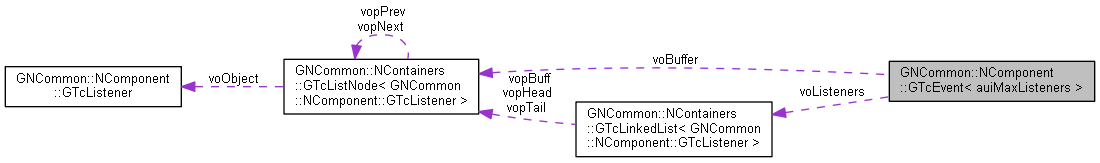
\includegraphics[width=350pt]{class_g_n_common_1_1_n_component_1_1_g_tc_event__coll__graph}
\end{center}
\end{figure}
\subsection*{Public Member Functions}
\begin{DoxyCompactItemize}
\item 
\mbox{\Hypertarget{class_g_n_common_1_1_n_component_1_1_g_tc_event_aa4b6f4ff1c4b91c55ac4c7350174bde8}\label{class_g_n_common_1_1_n_component_1_1_g_tc_event_aa4b6f4ff1c4b91c55ac4c7350174bde8}} 
void {\bfseries M\+Notify} (void $\ast$aop\+Sender, const \mbox{\hyperlink{namespace_g_n_common_a941b527ef318f318aed7903dc832b7e4}{Tu32}} aui\+Identifier)
\item 
\mbox{\Hypertarget{class_g_n_common_1_1_n_component_1_1_g_tc_event_adda36d639b1a0ddc31316559a1cddec9}\label{class_g_n_common_1_1_n_component_1_1_g_tc_event_adda36d639b1a0ddc31316559a1cddec9}} 
\mbox{\hyperlink{class_g_n_common_1_1_n_component_1_1_g_tc_event}{G\+Tc\+Event}} \& {\bfseries operator+=} (const \mbox{\hyperlink{class_g_n_common_1_1_n_component_1_1_g_tc_listener}{G\+Tc\+Listener}} \&aor\+Listener)
\item 
\mbox{\Hypertarget{class_g_n_common_1_1_n_component_1_1_g_tc_event_a5ecf841886dd8741f88ed053bb7c50ab}\label{class_g_n_common_1_1_n_component_1_1_g_tc_event_a5ecf841886dd8741f88ed053bb7c50ab}} 
\mbox{\hyperlink{class_g_n_common_1_1_n_component_1_1_g_tc_event}{G\+Tc\+Event}} \& {\bfseries operator-\/=} (const \mbox{\hyperlink{class_g_n_common_1_1_n_component_1_1_g_tc_listener}{G\+Tc\+Listener}} \&aor\+Listener)
\end{DoxyCompactItemize}
\subsection*{Protected Attributes}
\begin{DoxyCompactItemize}
\item 
\mbox{\Hypertarget{class_g_n_common_1_1_n_component_1_1_g_tc_event_ae060ae772a0689936a5ce21802e1766b}\label{class_g_n_common_1_1_n_component_1_1_g_tc_event_ae060ae772a0689936a5ce21802e1766b}} 
\mbox{\hyperlink{class_g_n_common_1_1_n_containers_1_1_g_tc_list_node}{G\+N\+Common\+::\+N\+Containers\+::\+G\+Tc\+List\+Node}}$<$ \mbox{\hyperlink{class_g_n_common_1_1_n_component_1_1_g_tc_listener}{G\+Tc\+Listener}} $>$ {\bfseries vo\+Buffer} \mbox{[}aui\+Max\+Listeners\mbox{]}
\item 
\mbox{\Hypertarget{class_g_n_common_1_1_n_component_1_1_g_tc_event_a4bdfc0245a63301bb4d6df850f066ef1}\label{class_g_n_common_1_1_n_component_1_1_g_tc_event_a4bdfc0245a63301bb4d6df850f066ef1}} 
\mbox{\hyperlink{class_g_n_common_1_1_n_containers_1_1_g_tc_linked_list}{G\+N\+Common\+::\+N\+Containers\+::\+G\+Tc\+Linked\+List}}$<$ \mbox{\hyperlink{class_g_n_common_1_1_n_component_1_1_g_tc_listener}{G\+Tc\+Listener}} $>$ {\bfseries vo\+Listeners}
\end{DoxyCompactItemize}


\subsection{Detailed Description}
\subsubsection*{template$<$Tu32 aui\+Max\+Listeners$>$\newline
class G\+N\+Common\+::\+N\+Component\+::\+G\+Tc\+Event$<$ aui\+Max\+Listeners $>$}



Definition at line \mbox{\hyperlink{_event_8h_source_l00014}{14}} of file \mbox{\hyperlink{_event_8h_source}{Event.\+h}}.



The documentation for this class was generated from the following file\+:\begin{DoxyCompactItemize}
\item 
C\+:/\+Users/edwar/\+Projects/\+Bergermeister\+Home/\+Software/\+Common/inc/\+Component/Event.\+h\end{DoxyCompactItemize}

\hypertarget{class_g_n_common_1_1_n_containers_1_1_g_tc_linked_list}{}\section{G\+N\+Common\+:\+:N\+Containers\+:\+:G\+Tc\+Linked\+List$<$ G\+Tc\+Type $>$ Class Template Reference}
\label{class_g_n_common_1_1_n_containers_1_1_g_tc_linked_list}\index{G\+N\+Common\+::\+N\+Containers\+::\+G\+Tc\+Linked\+List$<$ G\+Tc\+Type $>$@{G\+N\+Common\+::\+N\+Containers\+::\+G\+Tc\+Linked\+List$<$ G\+Tc\+Type $>$}}
\subsection*{Public Member Functions}
\begin{DoxyCompactItemize}
\item 
\mbox{\Hypertarget{class_g_n_common_1_1_n_containers_1_1_g_tc_linked_list_a3a573590845e357e8a8e6f70c3fd79d4}\label{class_g_n_common_1_1_n_containers_1_1_g_tc_linked_list_a3a573590845e357e8a8e6f70c3fd79d4}} 
void {\bfseries M\+Initialize} (\mbox{\hyperlink{class_g_n_common_1_1_n_containers_1_1_g_tc_list_node}{G\+Tc\+List\+Node}}$<$ G\+Tc\+Type $>$ $\ast$aop\+Buffer, \mbox{\hyperlink{namespace_g_n_common_a941b527ef318f318aed7903dc832b7e4}{Tu32}} aui\+Size)
\item 
\mbox{\Hypertarget{class_g_n_common_1_1_n_containers_1_1_g_tc_linked_list_af31039ab1077def5812bc7d61cd53d23}\label{class_g_n_common_1_1_n_containers_1_1_g_tc_linked_list_af31039ab1077def5812bc7d61cd53d23}} 
\mbox{\hyperlink{namespace_g_n_common_a8115dc7ed53b6e5b52e6bfde1632ea74}{Tb8}} {\bfseries M\+Is\+Initialized} (void) const
\item 
\mbox{\Hypertarget{class_g_n_common_1_1_n_containers_1_1_g_tc_linked_list_a8b10f43ce74f55d4e52bcecd39f244bf}\label{class_g_n_common_1_1_n_containers_1_1_g_tc_linked_list_a8b10f43ce74f55d4e52bcecd39f244bf}} 
\mbox{\hyperlink{namespace_g_n_common_a8115dc7ed53b6e5b52e6bfde1632ea74}{Tb8}} {\bfseries M\+Insert\+At\+Head} (G\+Tc\+Type \&aor\+Object)
\item 
\mbox{\Hypertarget{class_g_n_common_1_1_n_containers_1_1_g_tc_linked_list_a1119b8779eb4c7398e49f807eaffc23c}\label{class_g_n_common_1_1_n_containers_1_1_g_tc_linked_list_a1119b8779eb4c7398e49f807eaffc23c}} 
\mbox{\hyperlink{namespace_g_n_common_a8115dc7ed53b6e5b52e6bfde1632ea74}{Tb8}} {\bfseries M\+Insert\+At\+Tail} (G\+Tc\+Type \&aor\+Object)
\item 
\mbox{\Hypertarget{class_g_n_common_1_1_n_containers_1_1_g_tc_linked_list_a0a59862fc85d488e61e04978746f5d3f}\label{class_g_n_common_1_1_n_containers_1_1_g_tc_linked_list_a0a59862fc85d488e61e04978746f5d3f}} 
\mbox{\hyperlink{namespace_g_n_common_a8115dc7ed53b6e5b52e6bfde1632ea74}{Tb8}} {\bfseries M\+Insert} (G\+Tc\+Type \&aor\+Object)
\item 
\mbox{\Hypertarget{class_g_n_common_1_1_n_containers_1_1_g_tc_linked_list_ad12ca960896c194e92696e9f34c742a5}\label{class_g_n_common_1_1_n_containers_1_1_g_tc_linked_list_ad12ca960896c194e92696e9f34c742a5}} 
\mbox{\hyperlink{namespace_g_n_common_a8115dc7ed53b6e5b52e6bfde1632ea74}{Tb8}} {\bfseries M\+Remove\+Head} (void)
\item 
\mbox{\Hypertarget{class_g_n_common_1_1_n_containers_1_1_g_tc_linked_list_a222dd42866a883de1008866513a6ae76}\label{class_g_n_common_1_1_n_containers_1_1_g_tc_linked_list_a222dd42866a883de1008866513a6ae76}} 
\mbox{\hyperlink{namespace_g_n_common_a8115dc7ed53b6e5b52e6bfde1632ea74}{Tb8}} {\bfseries M\+Remove\+Tail} (void)
\item 
\mbox{\Hypertarget{class_g_n_common_1_1_n_containers_1_1_g_tc_linked_list_ac746f06616314b3638c25916b7102e74}\label{class_g_n_common_1_1_n_containers_1_1_g_tc_linked_list_ac746f06616314b3638c25916b7102e74}} 
\mbox{\hyperlink{namespace_g_n_common_a8115dc7ed53b6e5b52e6bfde1632ea74}{Tb8}} {\bfseries M\+Remove} (G\+Tc\+Type \&aor\+Object)
\end{DoxyCompactItemize}
\subsection*{Protected Attributes}
\begin{DoxyCompactItemize}
\item 
\mbox{\Hypertarget{class_g_n_common_1_1_n_containers_1_1_g_tc_linked_list_a4a0f308cf69f2cb7e86a01c0b32e77aa}\label{class_g_n_common_1_1_n_containers_1_1_g_tc_linked_list_a4a0f308cf69f2cb7e86a01c0b32e77aa}} 
\mbox{\hyperlink{class_g_n_common_1_1_n_containers_1_1_g_tc_list_node}{G\+Tc\+List\+Node}}$<$ G\+Tc\+Type $>$ $\ast$ {\bfseries vop\+Buff}
\item 
\mbox{\Hypertarget{class_g_n_common_1_1_n_containers_1_1_g_tc_linked_list_a86116504780ba3e48e4f3c88e6d2f827}\label{class_g_n_common_1_1_n_containers_1_1_g_tc_linked_list_a86116504780ba3e48e4f3c88e6d2f827}} 
\mbox{\hyperlink{class_g_n_common_1_1_n_containers_1_1_g_tc_list_node}{G\+Tc\+List\+Node}}$<$ G\+Tc\+Type $>$ $\ast$ {\bfseries vop\+Head}
\item 
\mbox{\Hypertarget{class_g_n_common_1_1_n_containers_1_1_g_tc_linked_list_a1773e394bf6b1eadeb37461ada2a737d}\label{class_g_n_common_1_1_n_containers_1_1_g_tc_linked_list_a1773e394bf6b1eadeb37461ada2a737d}} 
\mbox{\hyperlink{class_g_n_common_1_1_n_containers_1_1_g_tc_list_node}{G\+Tc\+List\+Node}}$<$ G\+Tc\+Type $>$ $\ast$ {\bfseries vop\+Tail}
\item 
\mbox{\Hypertarget{class_g_n_common_1_1_n_containers_1_1_g_tc_linked_list_a40e1149be848e39afe6bbfe31fed5015}\label{class_g_n_common_1_1_n_containers_1_1_g_tc_linked_list_a40e1149be848e39afe6bbfe31fed5015}} 
\mbox{\hyperlink{namespace_g_n_common_a941b527ef318f318aed7903dc832b7e4}{Tu32}} {\bfseries vui\+Size}
\item 
\mbox{\Hypertarget{class_g_n_common_1_1_n_containers_1_1_g_tc_linked_list_a720093251d1678a6a309976750d4215d}\label{class_g_n_common_1_1_n_containers_1_1_g_tc_linked_list_a720093251d1678a6a309976750d4215d}} 
\mbox{\hyperlink{namespace_g_n_common_a941b527ef318f318aed7903dc832b7e4}{Tu32}} {\bfseries vui\+Count}
\item 
\mbox{\Hypertarget{class_g_n_common_1_1_n_containers_1_1_g_tc_linked_list_a847dd5df95c4076a333745ce2aa1ff0d}\label{class_g_n_common_1_1_n_containers_1_1_g_tc_linked_list_a847dd5df95c4076a333745ce2aa1ff0d}} 
\mbox{\hyperlink{namespace_g_n_common_a8115dc7ed53b6e5b52e6bfde1632ea74}{Tb8}} {\bfseries vb\+Initialized}
\end{DoxyCompactItemize}


\subsection{Detailed Description}
\subsubsection*{template$<$class G\+Tc\+Type$>$\newline
class G\+N\+Common\+::\+N\+Containers\+::\+G\+Tc\+Linked\+List$<$ G\+Tc\+Type $>$}



Definition at line \mbox{\hyperlink{_linked_list_8h_source_l00011}{11}} of file \mbox{\hyperlink{_linked_list_8h_source}{Linked\+List.\+h}}.



The documentation for this class was generated from the following file\+:\begin{DoxyCompactItemize}
\item 
C\+:/\+Users/edwar/\+Projects/\+Bergermeister\+Home/\+Software/\+Common/inc/\+Containers/Linked\+List.\+h\end{DoxyCompactItemize}

\hypertarget{class_g_n_common_1_1_n_containers_1_1_g_tc_list}{}\section{G\+N\+Common\+:\+:N\+Containers\+:\+:G\+Tc\+List$<$ G\+Tc\+Type $>$ Class Template Reference}
\label{class_g_n_common_1_1_n_containers_1_1_g_tc_list}\index{G\+N\+Common\+::\+N\+Containers\+::\+G\+Tc\+List$<$ G\+Tc\+Type $>$@{G\+N\+Common\+::\+N\+Containers\+::\+G\+Tc\+List$<$ G\+Tc\+Type $>$}}
\subsection*{Public Member Functions}
\begin{DoxyCompactItemize}
\item 
\mbox{\Hypertarget{class_g_n_common_1_1_n_containers_1_1_g_tc_list_a3c9ac165409f6154366676e4895722e0}\label{class_g_n_common_1_1_n_containers_1_1_g_tc_list_a3c9ac165409f6154366676e4895722e0}} 
{\bfseries G\+Tc\+List} (G\+Tc\+Type $\ast$aop\+Buffer, const \mbox{\hyperlink{namespace_g_n_common_a941b527ef318f318aed7903dc832b7e4}{Tu32}} aui\+Capacity)
\item 
\mbox{\Hypertarget{class_g_n_common_1_1_n_containers_1_1_g_tc_list_a03513b89abcd069d6bf75a110edccccc}\label{class_g_n_common_1_1_n_containers_1_1_g_tc_list_a03513b89abcd069d6bf75a110edccccc}} 
{\bfseries G\+Tc\+List} (const \mbox{\hyperlink{class_g_n_common_1_1_n_containers_1_1_g_tc_list}{G\+Tc\+List}}$<$ G\+Tc\+Type $>$ \&aor\+List)
\item 
\mbox{\Hypertarget{class_g_n_common_1_1_n_containers_1_1_g_tc_list_a1af49ef8b3adc4a2537c316234e7cda0}\label{class_g_n_common_1_1_n_containers_1_1_g_tc_list_a1af49ef8b3adc4a2537c316234e7cda0}} 
virtual \mbox{\hyperlink{class_g_n_common_1_1_n_containers_1_1_g_tc_list}{G\+Tc\+List}}$<$ G\+Tc\+Type $>$ \& {\bfseries operator=} (const \mbox{\hyperlink{class_g_n_common_1_1_n_containers_1_1_g_tc_list}{G\+Tc\+List}}$<$ G\+Tc\+Type $>$ \&aor\+List)
\item 
\mbox{\Hypertarget{class_g_n_common_1_1_n_containers_1_1_g_tc_list_af0cba95288517ccfc2af1e34a0c17f2c}\label{class_g_n_common_1_1_n_containers_1_1_g_tc_list_af0cba95288517ccfc2af1e34a0c17f2c}} 
virtual \mbox{\hyperlink{namespace_g_n_common_a8115dc7ed53b6e5b52e6bfde1632ea74}{Tb8}} {\bfseries M\+Add} (const G\+Tc\+Type \&aor\+Item)
\item 
\mbox{\Hypertarget{class_g_n_common_1_1_n_containers_1_1_g_tc_list_ae630196feee0851049e7639ea41893d0}\label{class_g_n_common_1_1_n_containers_1_1_g_tc_list_ae630196feee0851049e7639ea41893d0}} 
virtual \mbox{\hyperlink{namespace_g_n_common_a8115dc7ed53b6e5b52e6bfde1632ea74}{Tb8}} {\bfseries M\+Insert} (const G\+Tc\+Type \&aor\+Item, const \mbox{\hyperlink{namespace_g_n_common_a941b527ef318f318aed7903dc832b7e4}{Tu32}} aui\+Index)
\item 
\mbox{\Hypertarget{class_g_n_common_1_1_n_containers_1_1_g_tc_list_a178bcd2cf41597e037833c03311b2c8f}\label{class_g_n_common_1_1_n_containers_1_1_g_tc_list_a178bcd2cf41597e037833c03311b2c8f}} 
virtual \mbox{\hyperlink{namespace_g_n_common_a8115dc7ed53b6e5b52e6bfde1632ea74}{Tb8}} {\bfseries M\+Remove} (const G\+Tc\+Type \&aor\+Item)
\item 
\mbox{\Hypertarget{class_g_n_common_1_1_n_containers_1_1_g_tc_list_ac79097e4228c07e7214b71dbf044c6c1}\label{class_g_n_common_1_1_n_containers_1_1_g_tc_list_ac79097e4228c07e7214b71dbf044c6c1}} 
virtual \mbox{\hyperlink{namespace_g_n_common_a8115dc7ed53b6e5b52e6bfde1632ea74}{Tb8}} {\bfseries M\+Remvoe\+At} (const \mbox{\hyperlink{namespace_g_n_common_a941b527ef318f318aed7903dc832b7e4}{Tu32}} aui\+Index)
\item 
\mbox{\Hypertarget{class_g_n_common_1_1_n_containers_1_1_g_tc_list_a14fb16ecd5edb7b231b127192e309c1f}\label{class_g_n_common_1_1_n_containers_1_1_g_tc_list_a14fb16ecd5edb7b231b127192e309c1f}} 
virtual void {\bfseries M\+Clear} (void)
\item 
\mbox{\Hypertarget{class_g_n_common_1_1_n_containers_1_1_g_tc_list_a1066bbf8bea38cc96ac00e72fdc01160}\label{class_g_n_common_1_1_n_containers_1_1_g_tc_list_a1066bbf8bea38cc96ac00e72fdc01160}} 
virtual \mbox{\hyperlink{namespace_g_n_common_a8115dc7ed53b6e5b52e6bfde1632ea74}{Tb8}} {\bfseries M\+Contains} (const G\+Tc\+Type \&aor\+Item) const
\item 
\mbox{\Hypertarget{class_g_n_common_1_1_n_containers_1_1_g_tc_list_af3515d6b8a1edeb6af7283784bb139a1}\label{class_g_n_common_1_1_n_containers_1_1_g_tc_list_af3515d6b8a1edeb6af7283784bb139a1}} 
virtual \mbox{\hyperlink{namespace_g_n_common_a941b527ef318f318aed7903dc832b7e4}{Tu32}} {\bfseries M\+Index\+Of} (const G\+Tc\+Type \&aor\+Item) const
\item 
\mbox{\Hypertarget{class_g_n_common_1_1_n_containers_1_1_g_tc_list_a6122791f6636a6e7018b0cfebd6978c6}\label{class_g_n_common_1_1_n_containers_1_1_g_tc_list_a6122791f6636a6e7018b0cfebd6978c6}} 
\mbox{\hyperlink{namespace_g_n_common_a941b527ef318f318aed7903dc832b7e4}{Tu32}} {\bfseries M\+Capacity} (void) const
\item 
\mbox{\Hypertarget{class_g_n_common_1_1_n_containers_1_1_g_tc_list_ac05103730e108c04b3945ee6ae320382}\label{class_g_n_common_1_1_n_containers_1_1_g_tc_list_ac05103730e108c04b3945ee6ae320382}} 
\mbox{\hyperlink{namespace_g_n_common_a941b527ef318f318aed7903dc832b7e4}{Tu32}} {\bfseries M\+Count} (void) const
\end{DoxyCompactItemize}
\subsection*{Public Attributes}
\begin{DoxyCompactItemize}
\item 
\mbox{\Hypertarget{class_g_n_common_1_1_n_containers_1_1_g_tc_list_a58c0d816076c5a58e0979799496af942}\label{class_g_n_common_1_1_n_containers_1_1_g_tc_list_a58c0d816076c5a58e0979799496af942}} 
G\+Tc\+Type $\ast$\& {\bfseries Vor\+Item}
\item 
\mbox{\Hypertarget{class_g_n_common_1_1_n_containers_1_1_g_tc_list_a9f78930e018406bc0240b9c5f023e994}\label{class_g_n_common_1_1_n_containers_1_1_g_tc_list_a9f78930e018406bc0240b9c5f023e994}} 
const \mbox{\hyperlink{namespace_g_n_common_a941b527ef318f318aed7903dc832b7e4}{Tu32}} \& {\bfseries Vuir\+Capacity}
\item 
\mbox{\Hypertarget{class_g_n_common_1_1_n_containers_1_1_g_tc_list_a9de552c7e334576676838a21971dd548}\label{class_g_n_common_1_1_n_containers_1_1_g_tc_list_a9de552c7e334576676838a21971dd548}} 
const \mbox{\hyperlink{namespace_g_n_common_a941b527ef318f318aed7903dc832b7e4}{Tu32}} \& {\bfseries Vuir\+Count}
\end{DoxyCompactItemize}
\subsection*{Protected Attributes}
\begin{DoxyCompactItemize}
\item 
\mbox{\Hypertarget{class_g_n_common_1_1_n_containers_1_1_g_tc_list_a059fe0982648142559d7c18603529848}\label{class_g_n_common_1_1_n_containers_1_1_g_tc_list_a059fe0982648142559d7c18603529848}} 
G\+Tc\+Type $\ast$ {\bfseries vop\+Buffer}
\item 
\mbox{\Hypertarget{class_g_n_common_1_1_n_containers_1_1_g_tc_list_aebcb9c4c9b69df72e6387b8afc6bd126}\label{class_g_n_common_1_1_n_containers_1_1_g_tc_list_aebcb9c4c9b69df72e6387b8afc6bd126}} 
\mbox{\hyperlink{namespace_g_n_common_a941b527ef318f318aed7903dc832b7e4}{Tu32}} {\bfseries vui\+Capacity}
\item 
\mbox{\Hypertarget{class_g_n_common_1_1_n_containers_1_1_g_tc_list_a2fad7e9af2e3ecbd6272ec044056fadf}\label{class_g_n_common_1_1_n_containers_1_1_g_tc_list_a2fad7e9af2e3ecbd6272ec044056fadf}} 
\mbox{\hyperlink{namespace_g_n_common_a941b527ef318f318aed7903dc832b7e4}{Tu32}} {\bfseries vui\+Count}
\end{DoxyCompactItemize}


\subsection{Detailed Description}
\subsubsection*{template$<$class G\+Tc\+Type$>$\newline
class G\+N\+Common\+::\+N\+Containers\+::\+G\+Tc\+List$<$ G\+Tc\+Type $>$}



Definition at line \mbox{\hyperlink{_list_8h_source_l00008}{8}} of file \mbox{\hyperlink{_list_8h_source}{List.\+h}}.



The documentation for this class was generated from the following file\+:\begin{DoxyCompactItemize}
\item 
C\+:/\+Projects/\+Bergermeister\+Home/\+Software/\+Common/inc/\+Containers/List.\+h\end{DoxyCompactItemize}

\hypertarget{class_g_n_common_1_1_n_component_1_1_g_tc_listener}{}\section{G\+N\+Common\+:\+:N\+Component\+:\+:G\+Tc\+Listener Class Reference}
\label{class_g_n_common_1_1_n_component_1_1_g_tc_listener}\index{G\+N\+Common\+::\+N\+Component\+::\+G\+Tc\+Listener@{G\+N\+Common\+::\+N\+Component\+::\+G\+Tc\+Listener}}
\subsection*{Public Types}
\begin{DoxyCompactItemize}
\item 
\mbox{\Hypertarget{class_g_n_common_1_1_n_component_1_1_g_tc_listener_a99a90bed304780bf96facc284bc6a3c8}\label{class_g_n_common_1_1_n_component_1_1_g_tc_listener_a99a90bed304780bf96facc284bc6a3c8}} 
typedef void($\ast$ {\bfseries Ts\+Handle}) (void $\ast$aop\+Listener, void $\ast$aop\+Parameter)
\end{DoxyCompactItemize}
\subsection*{Public Member Functions}
\begin{DoxyCompactItemize}
\item 
\mbox{\Hypertarget{class_g_n_common_1_1_n_component_1_1_g_tc_listener_aefc63ad4c7dc623de5c9c156848774ce}\label{class_g_n_common_1_1_n_component_1_1_g_tc_listener_aefc63ad4c7dc623de5c9c156848774ce}} 
{\bfseries G\+Tc\+Listener} (void $\ast$aop\+Instance, const Ts\+Handle aop\+Handle)
\item 
\mbox{\Hypertarget{class_g_n_common_1_1_n_component_1_1_g_tc_listener_aa7b293fa2d8fb08c31b9953557ead0c8}\label{class_g_n_common_1_1_n_component_1_1_g_tc_listener_aa7b293fa2d8fb08c31b9953557ead0c8}} 
void $\ast$ {\bfseries M\+Get\+Instance} (void) const
\item 
\mbox{\Hypertarget{class_g_n_common_1_1_n_component_1_1_g_tc_listener_a401b10e5fb60ecb19c6808ba5f758674}\label{class_g_n_common_1_1_n_component_1_1_g_tc_listener_a401b10e5fb60ecb19c6808ba5f758674}} 
Ts\+Handle {\bfseries M\+Get\+Handle} (void) const
\item 
\mbox{\Hypertarget{class_g_n_common_1_1_n_component_1_1_g_tc_listener_a4ae45f5ca3166a6cef67177b22ee478a}\label{class_g_n_common_1_1_n_component_1_1_g_tc_listener_a4ae45f5ca3166a6cef67177b22ee478a}} 
\mbox{\hyperlink{namespace_g_n_common_a8115dc7ed53b6e5b52e6bfde1632ea74}{Tb8}} {\bfseries operator==} (const \mbox{\hyperlink{class_g_n_common_1_1_n_component_1_1_g_tc_listener}{G\+Tc\+Listener}} \&aor\+Listener)
\end{DoxyCompactItemize}
\subsection*{Protected Attributes}
\begin{DoxyCompactItemize}
\item 
\mbox{\Hypertarget{class_g_n_common_1_1_n_component_1_1_g_tc_listener_ad2f8b2b212ee0120ce41c8715abe68aa}\label{class_g_n_common_1_1_n_component_1_1_g_tc_listener_ad2f8b2b212ee0120ce41c8715abe68aa}} 
void $\ast$ {\bfseries vop\+Instance}
\item 
\mbox{\Hypertarget{class_g_n_common_1_1_n_component_1_1_g_tc_listener_a0add5b70f2f2f400de4ab6442fe91595}\label{class_g_n_common_1_1_n_component_1_1_g_tc_listener_a0add5b70f2f2f400de4ab6442fe91595}} 
Ts\+Handle {\bfseries vop\+Handle}
\end{DoxyCompactItemize}


\subsection{Detailed Description}


Definition at line \mbox{\hyperlink{_listener_8h_source_l00007}{7}} of file \mbox{\hyperlink{_listener_8h_source}{Listener.\+h}}.



The documentation for this class was generated from the following files\+:\begin{DoxyCompactItemize}
\item 
C\+:/\+Users/edwar/\+Projects/\+Bergermeister\+Home/\+Software/\+Common/inc/\+Component/Listener.\+h\item 
C\+:/\+Users/edwar/\+Projects/\+Bergermeister\+Home/\+Software/\+Common/src/\+Component/Listener.\+cpp\end{DoxyCompactItemize}

\hypertarget{class_g_n_common_1_1_n_containers_1_1_g_tc_list_node}{}\section{G\+N\+Common\+:\+:N\+Containers\+:\+:G\+Tc\+List\+Node$<$ G\+Tc\+Type $>$ Class Template Reference}
\label{class_g_n_common_1_1_n_containers_1_1_g_tc_list_node}\index{G\+N\+Common\+::\+N\+Containers\+::\+G\+Tc\+List\+Node$<$ G\+Tc\+Type $>$@{G\+N\+Common\+::\+N\+Containers\+::\+G\+Tc\+List\+Node$<$ G\+Tc\+Type $>$}}
\subsection*{Public Member Functions}
\begin{DoxyCompactItemize}
\item 
\mbox{\Hypertarget{class_g_n_common_1_1_n_containers_1_1_g_tc_list_node_a86d95731366df231f1b666a1deea2452}\label{class_g_n_common_1_1_n_containers_1_1_g_tc_list_node_a86d95731366df231f1b666a1deea2452}} 
void {\bfseries M\+Set\+Object} (G\+Tc\+Type \&aor\+Object)
\item 
\mbox{\Hypertarget{class_g_n_common_1_1_n_containers_1_1_g_tc_list_node_a384f01990e3583745ad523f98cd9cb35}\label{class_g_n_common_1_1_n_containers_1_1_g_tc_list_node_a384f01990e3583745ad523f98cd9cb35}} 
G\+Tc\+Type $\ast$ {\bfseries M\+Get\+Object} (void)
\item 
\mbox{\Hypertarget{class_g_n_common_1_1_n_containers_1_1_g_tc_list_node_a732112aa53aa5c90521fa195023934da}\label{class_g_n_common_1_1_n_containers_1_1_g_tc_list_node_a732112aa53aa5c90521fa195023934da}} 
void {\bfseries M\+Set\+Next} (\mbox{\hyperlink{class_g_n_common_1_1_n_containers_1_1_g_tc_list_node}{G\+Tc\+List\+Node}}$<$ G\+Tc\+Type $>$ $\ast$aop\+Node)
\item 
\mbox{\Hypertarget{class_g_n_common_1_1_n_containers_1_1_g_tc_list_node_a09704031a826c226800f987aabef2dad}\label{class_g_n_common_1_1_n_containers_1_1_g_tc_list_node_a09704031a826c226800f987aabef2dad}} 
void {\bfseries M\+Set\+Prev} (\mbox{\hyperlink{class_g_n_common_1_1_n_containers_1_1_g_tc_list_node}{G\+Tc\+List\+Node}}$<$ G\+Tc\+Type $>$ $\ast$aop\+Node)
\item 
\mbox{\Hypertarget{class_g_n_common_1_1_n_containers_1_1_g_tc_list_node_a06b8ad652f01c74533b1058ce2d3d67f}\label{class_g_n_common_1_1_n_containers_1_1_g_tc_list_node_a06b8ad652f01c74533b1058ce2d3d67f}} 
\mbox{\hyperlink{class_g_n_common_1_1_n_containers_1_1_g_tc_list_node}{G\+Tc\+List\+Node}}$<$ G\+Tc\+Type $>$ $\ast$ {\bfseries M\+S\+Get\+Next} (void)
\item 
\mbox{\Hypertarget{class_g_n_common_1_1_n_containers_1_1_g_tc_list_node_aa5a14106ad0daa010bb195dd98b07785}\label{class_g_n_common_1_1_n_containers_1_1_g_tc_list_node_aa5a14106ad0daa010bb195dd98b07785}} 
\mbox{\hyperlink{class_g_n_common_1_1_n_containers_1_1_g_tc_list_node}{G\+Tc\+List\+Node}}$<$ G\+Tc\+Type $>$ $\ast$ {\bfseries M\+S\+Get\+Prev} (void)
\item 
\mbox{\Hypertarget{class_g_n_common_1_1_n_containers_1_1_g_tc_list_node_a5a961a5367a0bfafe93e0946e22e583f}\label{class_g_n_common_1_1_n_containers_1_1_g_tc_list_node_a5a961a5367a0bfafe93e0946e22e583f}} 
\mbox{\hyperlink{namespace_g_n_common_a8115dc7ed53b6e5b52e6bfde1632ea74}{Tb8}} {\bfseries M\+Insert\+After} (\mbox{\hyperlink{class_g_n_common_1_1_n_containers_1_1_g_tc_list_node}{G\+Tc\+List\+Node}}$<$ G\+Tc\+Type $>$ \&aor\+Node)
\item 
\mbox{\Hypertarget{class_g_n_common_1_1_n_containers_1_1_g_tc_list_node_a67448d9e550da3acb51a1469bb21fcf2}\label{class_g_n_common_1_1_n_containers_1_1_g_tc_list_node_a67448d9e550da3acb51a1469bb21fcf2}} 
\mbox{\hyperlink{namespace_g_n_common_a8115dc7ed53b6e5b52e6bfde1632ea74}{Tb8}} {\bfseries M\+Insert\+Before} (\mbox{\hyperlink{class_g_n_common_1_1_n_containers_1_1_g_tc_list_node}{G\+Tc\+List\+Node}}$<$ G\+Tc\+Type $>$ \&aor\+Node)
\item 
\mbox{\Hypertarget{class_g_n_common_1_1_n_containers_1_1_g_tc_list_node_a688a9ed0ea087b16d18d8bedaffa2299}\label{class_g_n_common_1_1_n_containers_1_1_g_tc_list_node_a688a9ed0ea087b16d18d8bedaffa2299}} 
\mbox{\hyperlink{namespace_g_n_common_a8115dc7ed53b6e5b52e6bfde1632ea74}{Tb8}} {\bfseries M\+Remove} (void)
\end{DoxyCompactItemize}
\subsection*{Protected Attributes}
\begin{DoxyCompactItemize}
\item 
\mbox{\Hypertarget{class_g_n_common_1_1_n_containers_1_1_g_tc_list_node_af93509661668861bd31387c744451143}\label{class_g_n_common_1_1_n_containers_1_1_g_tc_list_node_af93509661668861bd31387c744451143}} 
\mbox{\hyperlink{class_g_n_common_1_1_n_containers_1_1_g_tc_list_node}{G\+Tc\+List\+Node}}$<$ G\+Tc\+Type $>$ $\ast$ {\bfseries vop\+Next}
\item 
\mbox{\Hypertarget{class_g_n_common_1_1_n_containers_1_1_g_tc_list_node_aa5249ecdfe6ec1b7f0bd40df99fa071d}\label{class_g_n_common_1_1_n_containers_1_1_g_tc_list_node_aa5249ecdfe6ec1b7f0bd40df99fa071d}} 
\mbox{\hyperlink{class_g_n_common_1_1_n_containers_1_1_g_tc_list_node}{G\+Tc\+List\+Node}}$<$ G\+Tc\+Type $>$ $\ast$ {\bfseries vop\+Prev}
\item 
\mbox{\Hypertarget{class_g_n_common_1_1_n_containers_1_1_g_tc_list_node_addaf7e3067ae969fde633b63be203bf8}\label{class_g_n_common_1_1_n_containers_1_1_g_tc_list_node_addaf7e3067ae969fde633b63be203bf8}} 
G\+Tc\+Type {\bfseries vo\+Object}
\item 
\mbox{\Hypertarget{class_g_n_common_1_1_n_containers_1_1_g_tc_list_node_a44a4bdf6606a747e616753e68d211f76}\label{class_g_n_common_1_1_n_containers_1_1_g_tc_list_node_a44a4bdf6606a747e616753e68d211f76}} 
\mbox{\hyperlink{namespace_g_n_common_a8115dc7ed53b6e5b52e6bfde1632ea74}{Tb8}} {\bfseries vb\+Available}
\end{DoxyCompactItemize}


\subsection{Detailed Description}
\subsubsection*{template$<$class G\+Tc\+Type$>$\newline
class G\+N\+Common\+::\+N\+Containers\+::\+G\+Tc\+List\+Node$<$ G\+Tc\+Type $>$}



Definition at line \mbox{\hyperlink{_list_node_8h_source_l00011}{11}} of file \mbox{\hyperlink{_list_node_8h_source}{List\+Node.\+h}}.



The documentation for this class was generated from the following file\+:\begin{DoxyCompactItemize}
\item 
C\+:/\+Projects/\+Bergermeister\+Home/\+Software/\+Common/inc/\+Containers/List\+Node.\+h\end{DoxyCompactItemize}

\hypertarget{class_g_n_common_1_1_n_containers_1_1_g_tc_queue}{}\section{G\+N\+Common\+:\+:N\+Containers\+:\+:G\+Tc\+Queue$<$ G\+Tc\+Type $>$ Class Template Reference}
\label{class_g_n_common_1_1_n_containers_1_1_g_tc_queue}\index{G\+N\+Common\+::\+N\+Containers\+::\+G\+Tc\+Queue$<$ G\+Tc\+Type $>$@{G\+N\+Common\+::\+N\+Containers\+::\+G\+Tc\+Queue$<$ G\+Tc\+Type $>$}}
\subsection*{Public Member Functions}
\begin{DoxyCompactItemize}
\item 
\mbox{\Hypertarget{class_g_n_common_1_1_n_containers_1_1_g_tc_queue_aa64bd5892456166c0295ab054aa48839}\label{class_g_n_common_1_1_n_containers_1_1_g_tc_queue_aa64bd5892456166c0295ab054aa48839}} 
{\bfseries G\+Tc\+Queue} (G\+Tc\+Type $\ast$aop\+Buffer, \mbox{\hyperlink{namespace_g_n_common_a941b527ef318f318aed7903dc832b7e4}{Tu32}} aui\+Size)
\item 
\mbox{\Hypertarget{class_g_n_common_1_1_n_containers_1_1_g_tc_queue_a52d28010867f8ed0159b4d87d339623e}\label{class_g_n_common_1_1_n_containers_1_1_g_tc_queue_a52d28010867f8ed0159b4d87d339623e}} 
\mbox{\hyperlink{namespace_g_n_common_a8115dc7ed53b6e5b52e6bfde1632ea74}{Tb8}} {\bfseries M\+Enqueue} (G\+Tc\+Type \&aor\+Element)
\item 
\mbox{\Hypertarget{class_g_n_common_1_1_n_containers_1_1_g_tc_queue_a830d2f2082375430e547e0b99300a141}\label{class_g_n_common_1_1_n_containers_1_1_g_tc_queue_a830d2f2082375430e547e0b99300a141}} 
\mbox{\hyperlink{namespace_g_n_common_a8115dc7ed53b6e5b52e6bfde1632ea74}{Tb8}} {\bfseries M\+Dequeue} (G\+Tc\+Type \&aor\+Element)
\item 
\mbox{\Hypertarget{class_g_n_common_1_1_n_containers_1_1_g_tc_queue_ae4c9865a672f3e48f7cd0eab79cc42e0}\label{class_g_n_common_1_1_n_containers_1_1_g_tc_queue_ae4c9865a672f3e48f7cd0eab79cc42e0}} 
\mbox{\hyperlink{namespace_g_n_common_a8115dc7ed53b6e5b52e6bfde1632ea74}{Tb8}} {\bfseries M\+Is\+Empty} (void) const
\item 
\mbox{\Hypertarget{class_g_n_common_1_1_n_containers_1_1_g_tc_queue_a05c9cf6f2ae03fa910072560a4a19d28}\label{class_g_n_common_1_1_n_containers_1_1_g_tc_queue_a05c9cf6f2ae03fa910072560a4a19d28}} 
\mbox{\hyperlink{namespace_g_n_common_a8115dc7ed53b6e5b52e6bfde1632ea74}{Tb8}} {\bfseries M\+Is\+Full} (void) const
\item 
\mbox{\Hypertarget{class_g_n_common_1_1_n_containers_1_1_g_tc_queue_a9cae400d846f0ed6263e743cd452311a}\label{class_g_n_common_1_1_n_containers_1_1_g_tc_queue_a9cae400d846f0ed6263e743cd452311a}} 
\mbox{\hyperlink{namespace_g_n_common_a941b527ef318f318aed7903dc832b7e4}{Tu32}} {\bfseries M\+Count} (void) const
\end{DoxyCompactItemize}


\subsection{Detailed Description}
\subsubsection*{template$<$class G\+Tc\+Type$>$\newline
class G\+N\+Common\+::\+N\+Containers\+::\+G\+Tc\+Queue$<$ G\+Tc\+Type $>$}



Definition at line \mbox{\hyperlink{_queue_8h_source_l00008}{8}} of file \mbox{\hyperlink{_queue_8h_source}{Queue.\+h}}.



The documentation for this class was generated from the following file\+:\begin{DoxyCompactItemize}
\item 
C\+:/\+Users/edwar/\+Projects/\+Bergermeister\+Home/\+Software/\+Common/inc/\+Containers/Queue.\+h\end{DoxyCompactItemize}

\hypertarget{class_g_n_common_1_1_g_tc_stop_watch}{}\section{G\+N\+Common\+:\+:G\+Tc\+Stop\+Watch Class Reference}
\label{class_g_n_common_1_1_g_tc_stop_watch}\index{G\+N\+Common\+::\+G\+Tc\+Stop\+Watch@{G\+N\+Common\+::\+G\+Tc\+Stop\+Watch}}
\subsection*{Public Member Functions}
\begin{DoxyCompactItemize}
\item 
\mbox{\Hypertarget{class_g_n_common_1_1_g_tc_stop_watch_ae442c6e313df8f2ad22b4ceef71b89ab}\label{class_g_n_common_1_1_g_tc_stop_watch_ae442c6e313df8f2ad22b4ceef71b89ab}} 
{\bfseries G\+Tc\+Stop\+Watch} (const \mbox{\hyperlink{class_g_n_common_1_1_g_tc_stop_watch}{G\+Tc\+Stop\+Watch}} \&aor\+Stop\+Watch)
\item 
\mbox{\Hypertarget{class_g_n_common_1_1_g_tc_stop_watch_a334776e4f98289f2093b2da4cf3cb8b8}\label{class_g_n_common_1_1_g_tc_stop_watch_a334776e4f98289f2093b2da4cf3cb8b8}} 
\mbox{\hyperlink{class_g_n_common_1_1_g_tc_stop_watch}{G\+Tc\+Stop\+Watch}} \& {\bfseries operator=} (const \mbox{\hyperlink{class_g_n_common_1_1_g_tc_stop_watch}{G\+Tc\+Stop\+Watch}} \&aor\+Stop\+Watch)
\item 
\mbox{\Hypertarget{class_g_n_common_1_1_g_tc_stop_watch_ad62dfcb669827907489089ff31be6325}\label{class_g_n_common_1_1_g_tc_stop_watch_ad62dfcb669827907489089ff31be6325}} 
void {\bfseries M\+Start} (void)
\item 
\mbox{\Hypertarget{class_g_n_common_1_1_g_tc_stop_watch_ac9d0bf8c49268056b6b4d9486fdaade6}\label{class_g_n_common_1_1_g_tc_stop_watch_ac9d0bf8c49268056b6b4d9486fdaade6}} 
\mbox{\hyperlink{namespace_g_n_common_a01e8527dabf7ab4f123156b0701945eb}{G\+Tu64}} {\bfseries M\+Stop} (void)
\item 
\mbox{\Hypertarget{class_g_n_common_1_1_g_tc_stop_watch_a2fdbb8f6ed275c1601c2b52a530fd045}\label{class_g_n_common_1_1_g_tc_stop_watch_a2fdbb8f6ed275c1601c2b52a530fd045}} 
\mbox{\hyperlink{namespace_g_n_common_a01e8527dabf7ab4f123156b0701945eb}{G\+Tu64}} {\bfseries M\+Elapsed} (void)
\end{DoxyCompactItemize}
\subsection*{Protected Attributes}
\begin{DoxyCompactItemize}
\item 
\mbox{\Hypertarget{class_g_n_common_1_1_g_tc_stop_watch_a48e00f31a5f0d2ec9bf4678e3ea8bc0a}\label{class_g_n_common_1_1_g_tc_stop_watch_a48e00f31a5f0d2ec9bf4678e3ea8bc0a}} 
L\+A\+R\+G\+E\+\_\+\+I\+N\+T\+E\+G\+ER {\bfseries vo\+Start}
\item 
\mbox{\Hypertarget{class_g_n_common_1_1_g_tc_stop_watch_a0c7c046a1a57282bf389af72252410f6}\label{class_g_n_common_1_1_g_tc_stop_watch_a0c7c046a1a57282bf389af72252410f6}} 
L\+A\+R\+G\+E\+\_\+\+I\+N\+T\+E\+G\+ER {\bfseries vo\+End}
\item 
\mbox{\Hypertarget{class_g_n_common_1_1_g_tc_stop_watch_a8b50e42107f8f88743eea8856fe85dd5}\label{class_g_n_common_1_1_g_tc_stop_watch_a8b50e42107f8f88743eea8856fe85dd5}} 
\mbox{\hyperlink{namespace_g_n_common_a6b5283329f609e2175dd0c91fc1520ba}{G\+Tb8}} {\bfseries vb\+Running}
\end{DoxyCompactItemize}
\subsection*{Static Protected Attributes}
\begin{DoxyCompactItemize}
\item 
\mbox{\Hypertarget{class_g_n_common_1_1_g_tc_stop_watch_ae1b92efd901fed6c6de030fc9112a15f}\label{class_g_n_common_1_1_g_tc_stop_watch_ae1b92efd901fed6c6de030fc9112a15f}} 
static const L\+O\+N\+G\+L\+O\+NG {\bfseries xl\+Max\+Quad\+Part} = 9223372036854775807
\item 
\mbox{\Hypertarget{class_g_n_common_1_1_g_tc_stop_watch_ac9ff802e3258165d18f566ffe6bd6fc1}\label{class_g_n_common_1_1_g_tc_stop_watch_ac9ff802e3258165d18f566ffe6bd6fc1}} 
static const \mbox{\hyperlink{namespace_g_n_common_a01e8527dabf7ab4f123156b0701945eb}{G\+Tu64}} {\bfseries xul\+Time\+Base} = 1000000\+LL
\item 
\mbox{\Hypertarget{class_g_n_common_1_1_g_tc_stop_watch_afd7212375fb1201a16f966430dfcc30d}\label{class_g_n_common_1_1_g_tc_stop_watch_afd7212375fb1201a16f966430dfcc30d}} 
static \mbox{\hyperlink{namespace_g_n_common_a01e8527dabf7ab4f123156b0701945eb}{G\+Tu64}} {\bfseries vul\+Frequency} = 0
\end{DoxyCompactItemize}


\subsection{Detailed Description}


Definition at line 5 of file Stop\+Watch.\+h.



The documentation for this class was generated from the following files\+:\begin{DoxyCompactItemize}
\item 
C\+:/\+Projects/\+Bergermeister\+Home/\+Common/\+Source/Stop\+Watch.\+h\item 
C\+:/\+Projects/\+Bergermeister\+Home/\+Common/\+Source/Stop\+Watch.\+cpp\end{DoxyCompactItemize}

\hypertarget{class_g_n_common_1_1_n_notification_1_1_tc_alert}{}\section{G\+N\+Common\+:\+:N\+Notification\+:\+:Tc\+Alert Class Reference}
\label{class_g_n_common_1_1_n_notification_1_1_tc_alert}\index{G\+N\+Common\+::\+N\+Notification\+::\+Tc\+Alert@{G\+N\+Common\+::\+N\+Notification\+::\+Tc\+Alert}}


{\ttfamily \#include $<$Alert.\+h$>$}



Inheritance diagram for G\+N\+Common\+:\+:N\+Notification\+:\+:Tc\+Alert\+:
\nopagebreak
\begin{figure}[H]
\begin{center}
\leavevmode
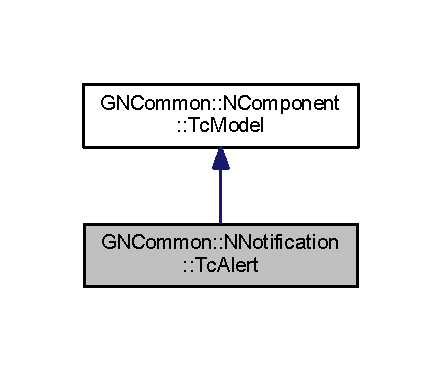
\includegraphics[width=212pt]{class_g_n_common_1_1_n_notification_1_1_tc_alert__inherit__graph}
\end{center}
\end{figure}


Collaboration diagram for G\+N\+Common\+:\+:N\+Notification\+:\+:Tc\+Alert\+:
\nopagebreak
\begin{figure}[H]
\begin{center}
\leavevmode
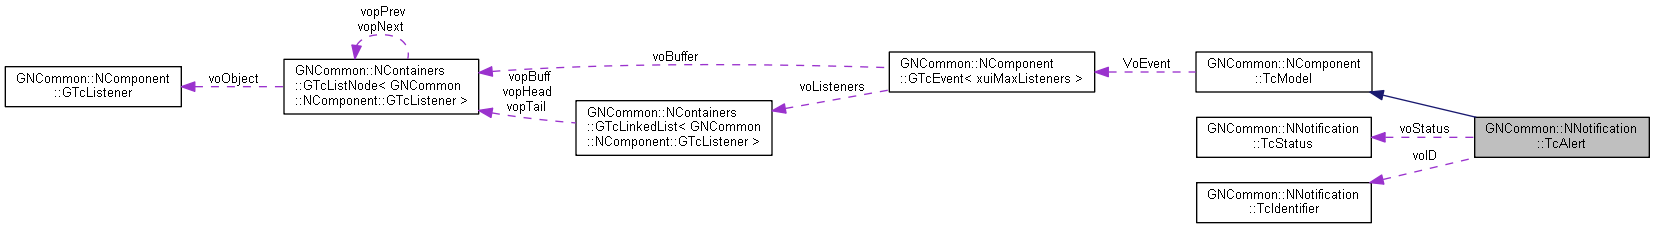
\includegraphics[width=350pt]{class_g_n_common_1_1_n_notification_1_1_tc_alert__coll__graph}
\end{center}
\end{figure}
\subsection*{Public Member Functions}
\begin{DoxyCompactItemize}
\item 
\mbox{\hyperlink{class_g_n_common_1_1_n_notification_1_1_tc_alert_a683af178a44e0ab7463c529d1ebb6d9c}{Tc\+Alert}} (void)
\item 
\mbox{\hyperlink{class_g_n_common_1_1_n_notification_1_1_tc_alert_abd42f842fe53942ed6d7a7008c3400c2}{$\sim$\+Tc\+Alert}} (void)
\item 
\mbox{\hyperlink{class_g_n_common_1_1_n_notification_1_1_tc_alert_a75120f1735cec51fe7f4afa519bd631b}{Tc\+Alert}} (const \mbox{\hyperlink{class_g_n_common_1_1_n_notification_1_1_tc_alert}{Tc\+Alert}} \&aor\+Alert)
\item 
\mbox{\hyperlink{class_g_n_common_1_1_n_notification_1_1_tc_alert}{Tc\+Alert}} \& \mbox{\hyperlink{class_g_n_common_1_1_n_notification_1_1_tc_alert_ad1371ff2988283b60a47c2879e1a0011}{operator=}} (const \mbox{\hyperlink{class_g_n_common_1_1_n_notification_1_1_tc_alert}{Tc\+Alert}} \&aor\+Alert)
\item 
void \mbox{\hyperlink{class_g_n_common_1_1_n_notification_1_1_tc_alert_a5411a5d9659282e199ceb16a1b88c17d}{M\+Set\+Identifier}} (const \mbox{\hyperlink{class_g_n_common_1_1_n_notification_1_1_tc_identifier}{Tc\+Identifier}} \&aor\+ID)
\item 
void \mbox{\hyperlink{class_g_n_common_1_1_n_notification_1_1_tc_alert_a682a17a50fc2c50bfb92ec3eeafdb5c9}{M\+Set\+Status}} (const \mbox{\hyperlink{class_g_n_common_1_1_n_notification_1_1_tc_status}{Tc\+Status}} \&aor\+Status)
\item 
void \mbox{\hyperlink{class_g_n_common_1_1_n_notification_1_1_tc_alert_ac6ed25087bcdbb12921d71c2c4126131}{M\+Set\+Timestamp}} (const \mbox{\hyperlink{namespace_g_n_common_a9404ee6090c788ae70aebd1436ceb97d}{Tu64}} aul\+Timestamp)
\item 
void \mbox{\hyperlink{class_g_n_common_1_1_n_notification_1_1_tc_alert_af4dccb7b428fdd2069a9dd1e6c12410b}{M\+Set\+Data}} (const \mbox{\hyperlink{namespace_g_n_common_a9404ee6090c788ae70aebd1436ceb97d}{Tu64}} aul\+Data)
\item 
\mbox{\hyperlink{class_g_n_common_1_1_n_notification_1_1_tc_identifier}{Tc\+Identifier}} \mbox{\hyperlink{class_g_n_common_1_1_n_notification_1_1_tc_alert_a3387c702b35bffddf5a480cdd52498aa}{M\+Get\+Identifier}} (void) const
\item 
\mbox{\hyperlink{class_g_n_common_1_1_n_notification_1_1_tc_status}{Tc\+Status}} \mbox{\hyperlink{class_g_n_common_1_1_n_notification_1_1_tc_alert_af6c3e9f29e796c2140dbe52229d439ca}{M\+Get\+Status}} (void) const
\item 
\mbox{\hyperlink{namespace_g_n_common_a9404ee6090c788ae70aebd1436ceb97d}{Tu64}} \mbox{\hyperlink{class_g_n_common_1_1_n_notification_1_1_tc_alert_a99c02af9bf2a17a34810ac5ed6be8856}{M\+Get\+Timestamp}} (void) const
\item 
\mbox{\hyperlink{namespace_g_n_common_a9404ee6090c788ae70aebd1436ceb97d}{Tu64}} \mbox{\hyperlink{class_g_n_common_1_1_n_notification_1_1_tc_alert_a4eeace6aa167a1b9b9a98487eee0ddb2}{M\+Get\+Data}} (void) const
\end{DoxyCompactItemize}
\subsection*{Static Public Attributes}
\begin{DoxyCompactItemize}
\item 
static const \mbox{\hyperlink{namespace_g_n_common_a941b527ef318f318aed7903dc832b7e4}{Tu32}} \mbox{\hyperlink{class_g_n_common_1_1_n_notification_1_1_tc_alert_a44f63050a2f1c7a4876a31ce2ffd2d06}{Xui\+Size\+Of\+Identifier}} = sizeof( \mbox{\hyperlink{class_g_n_common_1_1_n_notification_1_1_tc_identifier}{Tc\+Identifier}} )
\item 
static const \mbox{\hyperlink{namespace_g_n_common_a941b527ef318f318aed7903dc832b7e4}{Tu32}} \mbox{\hyperlink{class_g_n_common_1_1_n_notification_1_1_tc_alert_a59f856e0a33731ee0c235271bb013a34}{Xui\+Size\+Of\+Status}} = sizeof( \mbox{\hyperlink{class_g_n_common_1_1_n_notification_1_1_tc_status}{Tc\+Status}} )
\end{DoxyCompactItemize}
\subsection*{Protected Attributes}
\begin{DoxyCompactItemize}
\item 
\mbox{\hyperlink{class_g_n_common_1_1_n_notification_1_1_tc_identifier}{Tc\+Identifier}} \mbox{\hyperlink{class_g_n_common_1_1_n_notification_1_1_tc_alert_aa42573703fd6fa2ba90aa010fdc659ca}{vo\+ID}}
\item 
\mbox{\hyperlink{class_g_n_common_1_1_n_notification_1_1_tc_status}{Tc\+Status}} \mbox{\hyperlink{class_g_n_common_1_1_n_notification_1_1_tc_alert_ae993e1ea34de5347b08b21c9264cdb8e}{vo\+Status}}
\item 
\mbox{\hyperlink{namespace_g_n_common_a9404ee6090c788ae70aebd1436ceb97d}{Tu64}} \mbox{\hyperlink{class_g_n_common_1_1_n_notification_1_1_tc_alert_a3c6f656e3e526b9f97942188d7bb2930}{vul\+Timestamp}}
\item 
\mbox{\hyperlink{namespace_g_n_common_a9404ee6090c788ae70aebd1436ceb97d}{Tu64}} \mbox{\hyperlink{class_g_n_common_1_1_n_notification_1_1_tc_alert_ab49cb616a0e61e74234264d775a3408a}{vul\+Data}}
\end{DoxyCompactItemize}
\subsection*{Additional Inherited Members}


\subsection{Detailed Description}
Alert Class 

Definition at line \mbox{\hyperlink{_alert_8h_source_l00019}{19}} of file \mbox{\hyperlink{_alert_8h_source}{Alert.\+h}}.



\subsection{Constructor \& Destructor Documentation}
\mbox{\Hypertarget{class_g_n_common_1_1_n_notification_1_1_tc_alert_a683af178a44e0ab7463c529d1ebb6d9c}\label{class_g_n_common_1_1_n_notification_1_1_tc_alert_a683af178a44e0ab7463c529d1ebb6d9c}} 
\index{G\+N\+Common\+::\+N\+Notification\+::\+Tc\+Alert@{G\+N\+Common\+::\+N\+Notification\+::\+Tc\+Alert}!Tc\+Alert@{Tc\+Alert}}
\index{Tc\+Alert@{Tc\+Alert}!G\+N\+Common\+::\+N\+Notification\+::\+Tc\+Alert@{G\+N\+Common\+::\+N\+Notification\+::\+Tc\+Alert}}
\subsubsection{\texorpdfstring{Tc\+Alert()}{TcAlert()}\hspace{0.1cm}{\footnotesize\ttfamily [1/2]}}
{\footnotesize\ttfamily Tc\+Alert\+::\+Tc\+Alert (\begin{DoxyParamCaption}\item[{void}]{ }\end{DoxyParamCaption})}

Default Constructor 

Definition at line \mbox{\hyperlink{_alert_8cpp_source_l00013}{13}} of file \mbox{\hyperlink{_alert_8cpp_source}{Alert.\+cpp}}.

\mbox{\Hypertarget{class_g_n_common_1_1_n_notification_1_1_tc_alert_abd42f842fe53942ed6d7a7008c3400c2}\label{class_g_n_common_1_1_n_notification_1_1_tc_alert_abd42f842fe53942ed6d7a7008c3400c2}} 
\index{G\+N\+Common\+::\+N\+Notification\+::\+Tc\+Alert@{G\+N\+Common\+::\+N\+Notification\+::\+Tc\+Alert}!````~Tc\+Alert@{$\sim$\+Tc\+Alert}}
\index{````~Tc\+Alert@{$\sim$\+Tc\+Alert}!G\+N\+Common\+::\+N\+Notification\+::\+Tc\+Alert@{G\+N\+Common\+::\+N\+Notification\+::\+Tc\+Alert}}
\subsubsection{\texorpdfstring{$\sim$\+Tc\+Alert()}{~TcAlert()}}
{\footnotesize\ttfamily Tc\+Alert\+::$\sim$\+Tc\+Alert (\begin{DoxyParamCaption}\item[{void}]{ }\end{DoxyParamCaption})}

Default Destructor 

Definition at line \mbox{\hyperlink{_alert_8cpp_source_l00024}{24}} of file \mbox{\hyperlink{_alert_8cpp_source}{Alert.\+cpp}}.

\mbox{\Hypertarget{class_g_n_common_1_1_n_notification_1_1_tc_alert_a75120f1735cec51fe7f4afa519bd631b}\label{class_g_n_common_1_1_n_notification_1_1_tc_alert_a75120f1735cec51fe7f4afa519bd631b}} 
\index{G\+N\+Common\+::\+N\+Notification\+::\+Tc\+Alert@{G\+N\+Common\+::\+N\+Notification\+::\+Tc\+Alert}!Tc\+Alert@{Tc\+Alert}}
\index{Tc\+Alert@{Tc\+Alert}!G\+N\+Common\+::\+N\+Notification\+::\+Tc\+Alert@{G\+N\+Common\+::\+N\+Notification\+::\+Tc\+Alert}}
\subsubsection{\texorpdfstring{Tc\+Alert()}{TcAlert()}\hspace{0.1cm}{\footnotesize\ttfamily [2/2]}}
{\footnotesize\ttfamily Tc\+Alert\+::\+Tc\+Alert (\begin{DoxyParamCaption}\item[{const \mbox{\hyperlink{class_g_n_common_1_1_n_notification_1_1_tc_alert}{Tc\+Alert}} \&}]{aor\+Alert }\end{DoxyParamCaption})}

Copy Constructor 
\begin{DoxyParams}{Parameters}
{\em aor\+Alert} & Alert Constant Reference to copy \\
\hline
\end{DoxyParams}


Definition at line \mbox{\hyperlink{_alert_8cpp_source_l00033}{33}} of file \mbox{\hyperlink{_alert_8cpp_source}{Alert.\+cpp}}.



\subsection{Member Function Documentation}
\mbox{\Hypertarget{class_g_n_common_1_1_n_notification_1_1_tc_alert_a4eeace6aa167a1b9b9a98487eee0ddb2}\label{class_g_n_common_1_1_n_notification_1_1_tc_alert_a4eeace6aa167a1b9b9a98487eee0ddb2}} 
\index{G\+N\+Common\+::\+N\+Notification\+::\+Tc\+Alert@{G\+N\+Common\+::\+N\+Notification\+::\+Tc\+Alert}!M\+Get\+Data@{M\+Get\+Data}}
\index{M\+Get\+Data@{M\+Get\+Data}!G\+N\+Common\+::\+N\+Notification\+::\+Tc\+Alert@{G\+N\+Common\+::\+N\+Notification\+::\+Tc\+Alert}}
\subsubsection{\texorpdfstring{M\+Get\+Data()}{MGetData()}}
{\footnotesize\ttfamily \mbox{\hyperlink{namespace_g_n_common_a9404ee6090c788ae70aebd1436ceb97d}{Tu64}} Tc\+Alert\+::\+M\+Get\+Data (\begin{DoxyParamCaption}\item[{void}]{ }\end{DoxyParamCaption}) const}

M\+Get\+Trigger \begin{DoxyReturn}{Returns}
this-\/$>$vul\+Data constant 64-\/bit Integer Data 
\end{DoxyReturn}


Definition at line \mbox{\hyperlink{_alert_8cpp_source_l00136}{136}} of file \mbox{\hyperlink{_alert_8cpp_source}{Alert.\+cpp}}.

\mbox{\Hypertarget{class_g_n_common_1_1_n_notification_1_1_tc_alert_a3387c702b35bffddf5a480cdd52498aa}\label{class_g_n_common_1_1_n_notification_1_1_tc_alert_a3387c702b35bffddf5a480cdd52498aa}} 
\index{G\+N\+Common\+::\+N\+Notification\+::\+Tc\+Alert@{G\+N\+Common\+::\+N\+Notification\+::\+Tc\+Alert}!M\+Get\+Identifier@{M\+Get\+Identifier}}
\index{M\+Get\+Identifier@{M\+Get\+Identifier}!G\+N\+Common\+::\+N\+Notification\+::\+Tc\+Alert@{G\+N\+Common\+::\+N\+Notification\+::\+Tc\+Alert}}
\subsubsection{\texorpdfstring{M\+Get\+Identifier()}{MGetIdentifier()}}
{\footnotesize\ttfamily \mbox{\hyperlink{class_g_n_common_1_1_n_notification_1_1_tc_identifier}{Tc\+Identifier}} Tc\+Alert\+::\+M\+Get\+Identifier (\begin{DoxyParamCaption}\item[{void}]{ }\end{DoxyParamCaption}) const}

M\+Get\+Identifier \begin{DoxyReturn}{Returns}
this-\/$>$vo\+ID constant Ts\+Identifier 
\end{DoxyReturn}


Definition at line \mbox{\hyperlink{_alert_8cpp_source_l00109}{109}} of file \mbox{\hyperlink{_alert_8cpp_source}{Alert.\+cpp}}.

\mbox{\Hypertarget{class_g_n_common_1_1_n_notification_1_1_tc_alert_af6c3e9f29e796c2140dbe52229d439ca}\label{class_g_n_common_1_1_n_notification_1_1_tc_alert_af6c3e9f29e796c2140dbe52229d439ca}} 
\index{G\+N\+Common\+::\+N\+Notification\+::\+Tc\+Alert@{G\+N\+Common\+::\+N\+Notification\+::\+Tc\+Alert}!M\+Get\+Status@{M\+Get\+Status}}
\index{M\+Get\+Status@{M\+Get\+Status}!G\+N\+Common\+::\+N\+Notification\+::\+Tc\+Alert@{G\+N\+Common\+::\+N\+Notification\+::\+Tc\+Alert}}
\subsubsection{\texorpdfstring{M\+Get\+Status()}{MGetStatus()}}
{\footnotesize\ttfamily \mbox{\hyperlink{class_g_n_common_1_1_n_notification_1_1_tc_status}{Tc\+Status}} Tc\+Alert\+::\+M\+Get\+Status (\begin{DoxyParamCaption}\item[{void}]{ }\end{DoxyParamCaption}) const}

M\+Get\+Status \begin{DoxyReturn}{Returns}
this-\/$>$vo\+Status constant Ts\+Status 
\end{DoxyReturn}


Definition at line \mbox{\hyperlink{_alert_8cpp_source_l00118}{118}} of file \mbox{\hyperlink{_alert_8cpp_source}{Alert.\+cpp}}.

\mbox{\Hypertarget{class_g_n_common_1_1_n_notification_1_1_tc_alert_a99c02af9bf2a17a34810ac5ed6be8856}\label{class_g_n_common_1_1_n_notification_1_1_tc_alert_a99c02af9bf2a17a34810ac5ed6be8856}} 
\index{G\+N\+Common\+::\+N\+Notification\+::\+Tc\+Alert@{G\+N\+Common\+::\+N\+Notification\+::\+Tc\+Alert}!M\+Get\+Timestamp@{M\+Get\+Timestamp}}
\index{M\+Get\+Timestamp@{M\+Get\+Timestamp}!G\+N\+Common\+::\+N\+Notification\+::\+Tc\+Alert@{G\+N\+Common\+::\+N\+Notification\+::\+Tc\+Alert}}
\subsubsection{\texorpdfstring{M\+Get\+Timestamp()}{MGetTimestamp()}}
{\footnotesize\ttfamily \mbox{\hyperlink{namespace_g_n_common_a9404ee6090c788ae70aebd1436ceb97d}{Tu64}} Tc\+Alert\+::\+M\+Get\+Timestamp (\begin{DoxyParamCaption}\item[{void}]{ }\end{DoxyParamCaption}) const}

M\+Get\+Timestamp \begin{DoxyReturn}{Returns}
this-\/$>$vul\+Timestamp constant 64-\/bit Integer Timestamp 
\end{DoxyReturn}


Definition at line \mbox{\hyperlink{_alert_8cpp_source_l00127}{127}} of file \mbox{\hyperlink{_alert_8cpp_source}{Alert.\+cpp}}.

\mbox{\Hypertarget{class_g_n_common_1_1_n_notification_1_1_tc_alert_af4dccb7b428fdd2069a9dd1e6c12410b}\label{class_g_n_common_1_1_n_notification_1_1_tc_alert_af4dccb7b428fdd2069a9dd1e6c12410b}} 
\index{G\+N\+Common\+::\+N\+Notification\+::\+Tc\+Alert@{G\+N\+Common\+::\+N\+Notification\+::\+Tc\+Alert}!M\+Set\+Data@{M\+Set\+Data}}
\index{M\+Set\+Data@{M\+Set\+Data}!G\+N\+Common\+::\+N\+Notification\+::\+Tc\+Alert@{G\+N\+Common\+::\+N\+Notification\+::\+Tc\+Alert}}
\subsubsection{\texorpdfstring{M\+Set\+Data()}{MSetData()}}
{\footnotesize\ttfamily void Tc\+Alert\+::\+M\+Set\+Data (\begin{DoxyParamCaption}\item[{const \mbox{\hyperlink{namespace_g_n_common_a9404ee6090c788ae70aebd1436ceb97d}{Tu64}}}]{aul\+Data }\end{DoxyParamCaption})}

M\+Set\+Data 
\begin{DoxyParams}{Parameters}
{\em aul\+Data} & constant 64-\/bit Integer Data \\
\hline
\end{DoxyParams}


Definition at line \mbox{\hyperlink{_alert_8cpp_source_l00096}{96}} of file \mbox{\hyperlink{_alert_8cpp_source}{Alert.\+cpp}}.

Here is the caller graph for this function\+:
\nopagebreak
\begin{figure}[H]
\begin{center}
\leavevmode
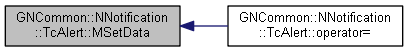
\includegraphics[width=350pt]{class_g_n_common_1_1_n_notification_1_1_tc_alert_af4dccb7b428fdd2069a9dd1e6c12410b_icgraph}
\end{center}
\end{figure}
\mbox{\Hypertarget{class_g_n_common_1_1_n_notification_1_1_tc_alert_a5411a5d9659282e199ceb16a1b88c17d}\label{class_g_n_common_1_1_n_notification_1_1_tc_alert_a5411a5d9659282e199ceb16a1b88c17d}} 
\index{G\+N\+Common\+::\+N\+Notification\+::\+Tc\+Alert@{G\+N\+Common\+::\+N\+Notification\+::\+Tc\+Alert}!M\+Set\+Identifier@{M\+Set\+Identifier}}
\index{M\+Set\+Identifier@{M\+Set\+Identifier}!G\+N\+Common\+::\+N\+Notification\+::\+Tc\+Alert@{G\+N\+Common\+::\+N\+Notification\+::\+Tc\+Alert}}
\subsubsection{\texorpdfstring{M\+Set\+Identifier()}{MSetIdentifier()}}
{\footnotesize\ttfamily void Tc\+Alert\+::\+M\+Set\+Identifier (\begin{DoxyParamCaption}\item[{const \mbox{\hyperlink{class_g_n_common_1_1_n_notification_1_1_tc_identifier}{Tc\+Identifier}} \&}]{aor\+ID }\end{DoxyParamCaption})}

M\+Set\+Identifier 
\begin{DoxyParams}{Parameters}
{\em aor\+ID} & Identifier Structure Constant Reference \\
\hline
\end{DoxyParams}


Definition at line \mbox{\hyperlink{_alert_8cpp_source_l00057}{57}} of file \mbox{\hyperlink{_alert_8cpp_source}{Alert.\+cpp}}.

Here is the caller graph for this function\+:
\nopagebreak
\begin{figure}[H]
\begin{center}
\leavevmode
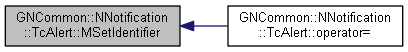
\includegraphics[width=350pt]{class_g_n_common_1_1_n_notification_1_1_tc_alert_a5411a5d9659282e199ceb16a1b88c17d_icgraph}
\end{center}
\end{figure}
\mbox{\Hypertarget{class_g_n_common_1_1_n_notification_1_1_tc_alert_a682a17a50fc2c50bfb92ec3eeafdb5c9}\label{class_g_n_common_1_1_n_notification_1_1_tc_alert_a682a17a50fc2c50bfb92ec3eeafdb5c9}} 
\index{G\+N\+Common\+::\+N\+Notification\+::\+Tc\+Alert@{G\+N\+Common\+::\+N\+Notification\+::\+Tc\+Alert}!M\+Set\+Status@{M\+Set\+Status}}
\index{M\+Set\+Status@{M\+Set\+Status}!G\+N\+Common\+::\+N\+Notification\+::\+Tc\+Alert@{G\+N\+Common\+::\+N\+Notification\+::\+Tc\+Alert}}
\subsubsection{\texorpdfstring{M\+Set\+Status()}{MSetStatus()}}
{\footnotesize\ttfamily void Tc\+Alert\+::\+M\+Set\+Status (\begin{DoxyParamCaption}\item[{const \mbox{\hyperlink{class_g_n_common_1_1_n_notification_1_1_tc_status}{Tc\+Status}} \&}]{aor\+Status }\end{DoxyParamCaption})}

M\+Set\+Status 
\begin{DoxyParams}{Parameters}
{\em aor\+Status} & Status Structure Constant Reference \\
\hline
\end{DoxyParams}


Definition at line \mbox{\hyperlink{_alert_8cpp_source_l00070}{70}} of file \mbox{\hyperlink{_alert_8cpp_source}{Alert.\+cpp}}.

Here is the caller graph for this function\+:
\nopagebreak
\begin{figure}[H]
\begin{center}
\leavevmode
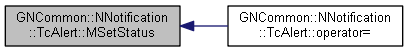
\includegraphics[width=350pt]{class_g_n_common_1_1_n_notification_1_1_tc_alert_a682a17a50fc2c50bfb92ec3eeafdb5c9_icgraph}
\end{center}
\end{figure}
\mbox{\Hypertarget{class_g_n_common_1_1_n_notification_1_1_tc_alert_ac6ed25087bcdbb12921d71c2c4126131}\label{class_g_n_common_1_1_n_notification_1_1_tc_alert_ac6ed25087bcdbb12921d71c2c4126131}} 
\index{G\+N\+Common\+::\+N\+Notification\+::\+Tc\+Alert@{G\+N\+Common\+::\+N\+Notification\+::\+Tc\+Alert}!M\+Set\+Timestamp@{M\+Set\+Timestamp}}
\index{M\+Set\+Timestamp@{M\+Set\+Timestamp}!G\+N\+Common\+::\+N\+Notification\+::\+Tc\+Alert@{G\+N\+Common\+::\+N\+Notification\+::\+Tc\+Alert}}
\subsubsection{\texorpdfstring{M\+Set\+Timestamp()}{MSetTimestamp()}}
{\footnotesize\ttfamily void Tc\+Alert\+::\+M\+Set\+Timestamp (\begin{DoxyParamCaption}\item[{const \mbox{\hyperlink{namespace_g_n_common_a9404ee6090c788ae70aebd1436ceb97d}{Tu64}}}]{aul\+Timestamp }\end{DoxyParamCaption})}

M\+Set\+Time\+Stamp 
\begin{DoxyParams}{Parameters}
{\em aul\+Timestamp} & constant 64-\/bit Integer Timestamp \\
\hline
\end{DoxyParams}


Definition at line \mbox{\hyperlink{_alert_8cpp_source_l00083}{83}} of file \mbox{\hyperlink{_alert_8cpp_source}{Alert.\+cpp}}.

Here is the caller graph for this function\+:
\nopagebreak
\begin{figure}[H]
\begin{center}
\leavevmode
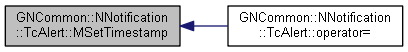
\includegraphics[width=350pt]{class_g_n_common_1_1_n_notification_1_1_tc_alert_ac6ed25087bcdbb12921d71c2c4126131_icgraph}
\end{center}
\end{figure}
\mbox{\Hypertarget{class_g_n_common_1_1_n_notification_1_1_tc_alert_ad1371ff2988283b60a47c2879e1a0011}\label{class_g_n_common_1_1_n_notification_1_1_tc_alert_ad1371ff2988283b60a47c2879e1a0011}} 
\index{G\+N\+Common\+::\+N\+Notification\+::\+Tc\+Alert@{G\+N\+Common\+::\+N\+Notification\+::\+Tc\+Alert}!operator=@{operator=}}
\index{operator=@{operator=}!G\+N\+Common\+::\+N\+Notification\+::\+Tc\+Alert@{G\+N\+Common\+::\+N\+Notification\+::\+Tc\+Alert}}
\subsubsection{\texorpdfstring{operator=()}{operator=()}}
{\footnotesize\ttfamily \mbox{\hyperlink{class_g_n_common_1_1_n_notification_1_1_tc_alert}{Tc\+Alert}} \& Tc\+Alert\+::operator= (\begin{DoxyParamCaption}\item[{const \mbox{\hyperlink{class_g_n_common_1_1_n_notification_1_1_tc_alert}{Tc\+Alert}} \&}]{aor\+Alert }\end{DoxyParamCaption})}

operator= Override 
\begin{DoxyParams}{Parameters}
{\em aor\+Alert} & Alert Constant Reference to copy \\
\hline
\end{DoxyParams}
\begin{DoxyReturn}{Returns}
$\ast$this G\+Tc\+Alert Reference 
\end{DoxyReturn}


Definition at line \mbox{\hyperlink{_alert_8cpp_source_l00043}{43}} of file \mbox{\hyperlink{_alert_8cpp_source}{Alert.\+cpp}}.

Here is the call graph for this function\+:
\nopagebreak
\begin{figure}[H]
\begin{center}
\leavevmode
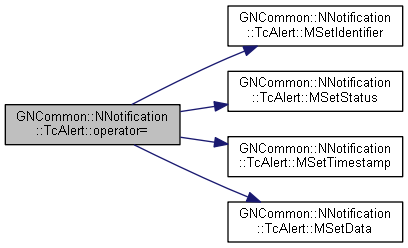
\includegraphics[width=350pt]{class_g_n_common_1_1_n_notification_1_1_tc_alert_ad1371ff2988283b60a47c2879e1a0011_cgraph}
\end{center}
\end{figure}


\subsection{Member Data Documentation}
\mbox{\Hypertarget{class_g_n_common_1_1_n_notification_1_1_tc_alert_aa42573703fd6fa2ba90aa010fdc659ca}\label{class_g_n_common_1_1_n_notification_1_1_tc_alert_aa42573703fd6fa2ba90aa010fdc659ca}} 
\index{G\+N\+Common\+::\+N\+Notification\+::\+Tc\+Alert@{G\+N\+Common\+::\+N\+Notification\+::\+Tc\+Alert}!vo\+ID@{vo\+ID}}
\index{vo\+ID@{vo\+ID}!G\+N\+Common\+::\+N\+Notification\+::\+Tc\+Alert@{G\+N\+Common\+::\+N\+Notification\+::\+Tc\+Alert}}
\subsubsection{\texorpdfstring{vo\+ID}{voID}}
{\footnotesize\ttfamily \mbox{\hyperlink{class_g_n_common_1_1_n_notification_1_1_tc_identifier}{Tc\+Identifier}} G\+N\+Common\+::\+N\+Notification\+::\+Tc\+Alert\+::vo\+ID\hspace{0.3cm}{\ttfamily [protected]}}

Encoded Identifier 

Definition at line \mbox{\hyperlink{_alert_8h_source_l00026}{26}} of file \mbox{\hyperlink{_alert_8h_source}{Alert.\+h}}.

\mbox{\Hypertarget{class_g_n_common_1_1_n_notification_1_1_tc_alert_ae993e1ea34de5347b08b21c9264cdb8e}\label{class_g_n_common_1_1_n_notification_1_1_tc_alert_ae993e1ea34de5347b08b21c9264cdb8e}} 
\index{G\+N\+Common\+::\+N\+Notification\+::\+Tc\+Alert@{G\+N\+Common\+::\+N\+Notification\+::\+Tc\+Alert}!vo\+Status@{vo\+Status}}
\index{vo\+Status@{vo\+Status}!G\+N\+Common\+::\+N\+Notification\+::\+Tc\+Alert@{G\+N\+Common\+::\+N\+Notification\+::\+Tc\+Alert}}
\subsubsection{\texorpdfstring{vo\+Status}{voStatus}}
{\footnotesize\ttfamily \mbox{\hyperlink{class_g_n_common_1_1_n_notification_1_1_tc_status}{Tc\+Status}} G\+N\+Common\+::\+N\+Notification\+::\+Tc\+Alert\+::vo\+Status\hspace{0.3cm}{\ttfamily [protected]}}

Encoded Status 

Definition at line \mbox{\hyperlink{_alert_8h_source_l00027}{27}} of file \mbox{\hyperlink{_alert_8h_source}{Alert.\+h}}.

\mbox{\Hypertarget{class_g_n_common_1_1_n_notification_1_1_tc_alert_ab49cb616a0e61e74234264d775a3408a}\label{class_g_n_common_1_1_n_notification_1_1_tc_alert_ab49cb616a0e61e74234264d775a3408a}} 
\index{G\+N\+Common\+::\+N\+Notification\+::\+Tc\+Alert@{G\+N\+Common\+::\+N\+Notification\+::\+Tc\+Alert}!vul\+Data@{vul\+Data}}
\index{vul\+Data@{vul\+Data}!G\+N\+Common\+::\+N\+Notification\+::\+Tc\+Alert@{G\+N\+Common\+::\+N\+Notification\+::\+Tc\+Alert}}
\subsubsection{\texorpdfstring{vul\+Data}{vulData}}
{\footnotesize\ttfamily \mbox{\hyperlink{namespace_g_n_common_a9404ee6090c788ae70aebd1436ceb97d}{Tu64}} G\+N\+Common\+::\+N\+Notification\+::\+Tc\+Alert\+::vul\+Data\hspace{0.3cm}{\ttfamily [protected]}}

64-\/bit Additional Data 

Definition at line \mbox{\hyperlink{_alert_8h_source_l00029}{29}} of file \mbox{\hyperlink{_alert_8h_source}{Alert.\+h}}.

\mbox{\Hypertarget{class_g_n_common_1_1_n_notification_1_1_tc_alert_a3c6f656e3e526b9f97942188d7bb2930}\label{class_g_n_common_1_1_n_notification_1_1_tc_alert_a3c6f656e3e526b9f97942188d7bb2930}} 
\index{G\+N\+Common\+::\+N\+Notification\+::\+Tc\+Alert@{G\+N\+Common\+::\+N\+Notification\+::\+Tc\+Alert}!vul\+Timestamp@{vul\+Timestamp}}
\index{vul\+Timestamp@{vul\+Timestamp}!G\+N\+Common\+::\+N\+Notification\+::\+Tc\+Alert@{G\+N\+Common\+::\+N\+Notification\+::\+Tc\+Alert}}
\subsubsection{\texorpdfstring{vul\+Timestamp}{vulTimestamp}}
{\footnotesize\ttfamily \mbox{\hyperlink{namespace_g_n_common_a9404ee6090c788ae70aebd1436ceb97d}{Tu64}} G\+N\+Common\+::\+N\+Notification\+::\+Tc\+Alert\+::vul\+Timestamp\hspace{0.3cm}{\ttfamily [protected]}}

64-\/bit Timestamp of Occurrence 

Definition at line \mbox{\hyperlink{_alert_8h_source_l00028}{28}} of file \mbox{\hyperlink{_alert_8h_source}{Alert.\+h}}.

\mbox{\Hypertarget{class_g_n_common_1_1_n_notification_1_1_tc_alert_a44f63050a2f1c7a4876a31ce2ffd2d06}\label{class_g_n_common_1_1_n_notification_1_1_tc_alert_a44f63050a2f1c7a4876a31ce2ffd2d06}} 
\index{G\+N\+Common\+::\+N\+Notification\+::\+Tc\+Alert@{G\+N\+Common\+::\+N\+Notification\+::\+Tc\+Alert}!Xui\+Size\+Of\+Identifier@{Xui\+Size\+Of\+Identifier}}
\index{Xui\+Size\+Of\+Identifier@{Xui\+Size\+Of\+Identifier}!G\+N\+Common\+::\+N\+Notification\+::\+Tc\+Alert@{G\+N\+Common\+::\+N\+Notification\+::\+Tc\+Alert}}
\subsubsection{\texorpdfstring{Xui\+Size\+Of\+Identifier}{XuiSizeOfIdentifier}}
{\footnotesize\ttfamily const \mbox{\hyperlink{namespace_g_n_common_a941b527ef318f318aed7903dc832b7e4}{Tu32}} G\+N\+Common\+::\+N\+Notification\+::\+Tc\+Alert\+::\+Xui\+Size\+Of\+Identifier = sizeof( \mbox{\hyperlink{class_g_n_common_1_1_n_notification_1_1_tc_identifier}{Tc\+Identifier}} )\hspace{0.3cm}{\ttfamily [static]}}

Size of Identifier 

Definition at line \mbox{\hyperlink{_alert_8h_source_l00022}{22}} of file \mbox{\hyperlink{_alert_8h_source}{Alert.\+h}}.

\mbox{\Hypertarget{class_g_n_common_1_1_n_notification_1_1_tc_alert_a59f856e0a33731ee0c235271bb013a34}\label{class_g_n_common_1_1_n_notification_1_1_tc_alert_a59f856e0a33731ee0c235271bb013a34}} 
\index{G\+N\+Common\+::\+N\+Notification\+::\+Tc\+Alert@{G\+N\+Common\+::\+N\+Notification\+::\+Tc\+Alert}!Xui\+Size\+Of\+Status@{Xui\+Size\+Of\+Status}}
\index{Xui\+Size\+Of\+Status@{Xui\+Size\+Of\+Status}!G\+N\+Common\+::\+N\+Notification\+::\+Tc\+Alert@{G\+N\+Common\+::\+N\+Notification\+::\+Tc\+Alert}}
\subsubsection{\texorpdfstring{Xui\+Size\+Of\+Status}{XuiSizeOfStatus}}
{\footnotesize\ttfamily const \mbox{\hyperlink{namespace_g_n_common_a941b527ef318f318aed7903dc832b7e4}{Tu32}} G\+N\+Common\+::\+N\+Notification\+::\+Tc\+Alert\+::\+Xui\+Size\+Of\+Status = sizeof( \mbox{\hyperlink{class_g_n_common_1_1_n_notification_1_1_tc_status}{Tc\+Status}} )\hspace{0.3cm}{\ttfamily [static]}}

Size of Status 

Definition at line \mbox{\hyperlink{_alert_8h_source_l00023}{23}} of file \mbox{\hyperlink{_alert_8h_source}{Alert.\+h}}.



The documentation for this class was generated from the following files\+:\begin{DoxyCompactItemize}
\item 
C\+:/\+Users/edwar/\+Projects/\+Bergermeister\+Home/\+Software/\+Common/inc/\+Notification/\mbox{\hyperlink{_alert_8h}{Alert.\+h}}\item 
C\+:/\+Users/edwar/\+Projects/\+Bergermeister\+Home/\+Software/\+Common/src/\+Notification/Alert.\+cpp\end{DoxyCompactItemize}

\hypertarget{class_g_n_common_1_1_n_data_authentication_1_1_tc_c_r_c32}{}\section{G\+N\+Common\+:\+:N\+Data\+Authentication\+:\+:Tc\+C\+R\+C32 Class Reference}
\label{class_g_n_common_1_1_n_data_authentication_1_1_tc_c_r_c32}\index{G\+N\+Common\+::\+N\+Data\+Authentication\+::\+Tc\+C\+R\+C32@{G\+N\+Common\+::\+N\+Data\+Authentication\+::\+Tc\+C\+R\+C32}}


32-\/bit Cycle Redundancy Code (C\+RC) Class  




{\ttfamily \#include $<$C\+R\+C32.\+h$>$}

\subsection*{Public Member Functions}
\begin{DoxyCompactItemize}
\item 
\mbox{\Hypertarget{class_g_n_common_1_1_n_data_authentication_1_1_tc_c_r_c32_a125172ccc1307fdeb7bf1d4dc95673da}\label{class_g_n_common_1_1_n_data_authentication_1_1_tc_c_r_c32_a125172ccc1307fdeb7bf1d4dc95673da}} 
{\bfseries Tc\+C\+R\+C32} (const \mbox{\hyperlink{class_g_n_common_1_1_n_data_authentication_1_1_tc_c_r_c32}{Tc\+C\+R\+C32}} \&aor\+C\+RC)
\item 
\mbox{\Hypertarget{class_g_n_common_1_1_n_data_authentication_1_1_tc_c_r_c32_a96fe7f4bb468dbab57189c5d9a39e3f4}\label{class_g_n_common_1_1_n_data_authentication_1_1_tc_c_r_c32_a96fe7f4bb468dbab57189c5d9a39e3f4}} 
\mbox{\hyperlink{class_g_n_common_1_1_n_data_authentication_1_1_tc_c_r_c32}{Tc\+C\+R\+C32}} \& {\bfseries operator=} (const \mbox{\hyperlink{class_g_n_common_1_1_n_data_authentication_1_1_tc_c_r_c32}{Tc\+C\+R\+C32}} \&aor\+C\+RC)
\item 
\mbox{\Hypertarget{class_g_n_common_1_1_n_data_authentication_1_1_tc_c_r_c32_a170f6f898b26087d694d0e5163d4016b}\label{class_g_n_common_1_1_n_data_authentication_1_1_tc_c_r_c32_a170f6f898b26087d694d0e5163d4016b}} 
\mbox{\hyperlink{namespace_g_n_common_a941b527ef318f318aed7903dc832b7e4}{Tu32}} {\bfseries M\+Get} (const \mbox{\hyperlink{namespace_g_n_common_a7939e251ddbf5d3a31832dcfdc8bde39}{Tu8}} $\ast$aucp\+Buffer, const \mbox{\hyperlink{namespace_g_n_common_a941b527ef318f318aed7903dc832b7e4}{Tu32}} aui\+Bytes, const \mbox{\hyperlink{namespace_g_n_common_a941b527ef318f318aed7903dc832b7e4}{Tu32}} aui\+Seed=\mbox{\hyperlink{class_g_n_common_1_1_n_data_authentication_1_1_tc_c_r_c32_a07c2c3cd02a6f0eedc7a56565f7960c1}{xui\+Default\+Seed}}, const \mbox{\hyperlink{namespace_g_n_common_a941b527ef318f318aed7903dc832b7e4}{Tu32}} aui\+Table\mbox{[}\mbox{\hyperlink{class_g_n_common_1_1_n_data_authentication_1_1_tc_c_r_c32_a520aaabe0f4ade7f38afd480281b2180}{Xui\+Table\+Size}}\mbox{]}=\mbox{\hyperlink{class_g_n_common_1_1_n_data_authentication_1_1_tc_c_r_c32_a4aafd40037856d1bd4ea6f6ce0928836}{xui\+Table}}) const
\item 
\mbox{\Hypertarget{class_g_n_common_1_1_n_data_authentication_1_1_tc_c_r_c32_a8d798a894e55e69f847392f72fc2e84d}\label{class_g_n_common_1_1_n_data_authentication_1_1_tc_c_r_c32_a8d798a894e55e69f847392f72fc2e84d}} 
\mbox{\hyperlink{namespace_g_n_common_a8115dc7ed53b6e5b52e6bfde1632ea74}{Tb8}} {\bfseries M\+Verify} (void) const
\item 
void \mbox{\hyperlink{class_g_n_common_1_1_n_data_authentication_1_1_tc_c_r_c32_a11a20f9425a6431b0f2eb72e126a3a0e}{M\+Generate\+Table}} (\mbox{\hyperlink{namespace_g_n_common_a941b527ef318f318aed7903dc832b7e4}{Tu32}} aui\+Table\mbox{[}\mbox{\hyperlink{class_g_n_common_1_1_n_data_authentication_1_1_tc_c_r_c32_a520aaabe0f4ade7f38afd480281b2180}{Xui\+Table\+Size}}\mbox{]}, const \mbox{\hyperlink{namespace_g_n_common_a941b527ef318f318aed7903dc832b7e4}{Tu32}} aui\+Polynomial=\mbox{\hyperlink{class_g_n_common_1_1_n_data_authentication_1_1_tc_c_r_c32_ab4394051ff10830de29fa62cbb6f1490}{Xui\+Polynomial}})
\begin{DoxyCompactList}\small\item\em Generate a C\+RC Lookup Table. \end{DoxyCompactList}\item 
\mbox{\hyperlink{namespace_g_n_common_a8115dc7ed53b6e5b52e6bfde1632ea74}{Tb8}} \mbox{\hyperlink{class_g_n_common_1_1_n_data_authentication_1_1_tc_c_r_c32_a2f822ac900cdba0a94b8e9361eb86b5c}{M\+Compare\+Table}} (const \mbox{\hyperlink{namespace_g_n_common_a941b527ef318f318aed7903dc832b7e4}{Tu32}} aui\+Table\mbox{[}\mbox{\hyperlink{class_g_n_common_1_1_n_data_authentication_1_1_tc_c_r_c32_a520aaabe0f4ade7f38afd480281b2180}{Xui\+Table\+Size}}\mbox{]})
\begin{DoxyCompactList}\small\item\em Compares the lookup table. \end{DoxyCompactList}\end{DoxyCompactItemize}
\subsection*{Static Public Attributes}
\begin{DoxyCompactItemize}
\item 
static const \mbox{\hyperlink{namespace_g_n_common_a941b527ef318f318aed7903dc832b7e4}{Tu32}} \mbox{\hyperlink{class_g_n_common_1_1_n_data_authentication_1_1_tc_c_r_c32_a520aaabe0f4ade7f38afd480281b2180}{Xui\+Table\+Size}} = 256
\item 
static const \mbox{\hyperlink{namespace_g_n_common_a941b527ef318f318aed7903dc832b7e4}{Tu32}} \mbox{\hyperlink{class_g_n_common_1_1_n_data_authentication_1_1_tc_c_r_c32_ab4394051ff10830de29fa62cbb6f1490}{Xui\+Polynomial}} = 0x\+E\+D\+B88320
\end{DoxyCompactItemize}
\subsection*{Static Protected Attributes}
\begin{DoxyCompactItemize}
\item 
static const \mbox{\hyperlink{namespace_g_n_common_a941b527ef318f318aed7903dc832b7e4}{Tu32}} \mbox{\hyperlink{class_g_n_common_1_1_n_data_authentication_1_1_tc_c_r_c32_a07c2c3cd02a6f0eedc7a56565f7960c1}{xui\+Default\+Seed}} = 0x\+F\+F\+F\+F\+F\+F\+FF
\item 
static const \mbox{\hyperlink{namespace_g_n_common_a941b527ef318f318aed7903dc832b7e4}{Tu32}} \mbox{\hyperlink{class_g_n_common_1_1_n_data_authentication_1_1_tc_c_r_c32_aafa160e99ae03386b426884450ba3796}{xui\+Table\+C\+RC}} = 0x6\+F\+C\+F9\+E13
\item 
static const \mbox{\hyperlink{namespace_g_n_common_a941b527ef318f318aed7903dc832b7e4}{Tu32}} \mbox{\hyperlink{class_g_n_common_1_1_n_data_authentication_1_1_tc_c_r_c32_aae1c17e2c8f312d0bf2e062a5412ada8}{xui\+Shift8}} = 8
\item 
static const \mbox{\hyperlink{namespace_g_n_common_a941b527ef318f318aed7903dc832b7e4}{Tu32}} \mbox{\hyperlink{class_g_n_common_1_1_n_data_authentication_1_1_tc_c_r_c32_ab156bd5eaab2fe267499870a8f6e4925}{xui\+Mask\+Byte}} = 0x000000\+FF
\item 
static const \mbox{\hyperlink{namespace_g_n_common_a941b527ef318f318aed7903dc832b7e4}{Tu32}} \mbox{\hyperlink{class_g_n_common_1_1_n_data_authentication_1_1_tc_c_r_c32_a4aafd40037856d1bd4ea6f6ce0928836}{xui\+Table}} \mbox{[}\mbox{\hyperlink{class_g_n_common_1_1_n_data_authentication_1_1_tc_c_r_c32_a520aaabe0f4ade7f38afd480281b2180}{Xui\+Table\+Size}}\mbox{]}
\end{DoxyCompactItemize}


\subsection{Detailed Description}
32-\/bit Cycle Redundancy Code (C\+RC) Class 

Definition at line \mbox{\hyperlink{_c_r_c32_8h_source_l00015}{15}} of file \mbox{\hyperlink{_c_r_c32_8h_source}{C\+R\+C32.\+h}}.



\subsection{Member Function Documentation}
\mbox{\Hypertarget{class_g_n_common_1_1_n_data_authentication_1_1_tc_c_r_c32_a2f822ac900cdba0a94b8e9361eb86b5c}\label{class_g_n_common_1_1_n_data_authentication_1_1_tc_c_r_c32_a2f822ac900cdba0a94b8e9361eb86b5c}} 
\index{G\+N\+Common\+::\+N\+Data\+Authentication\+::\+Tc\+C\+R\+C32@{G\+N\+Common\+::\+N\+Data\+Authentication\+::\+Tc\+C\+R\+C32}!M\+Compare\+Table@{M\+Compare\+Table}}
\index{M\+Compare\+Table@{M\+Compare\+Table}!G\+N\+Common\+::\+N\+Data\+Authentication\+::\+Tc\+C\+R\+C32@{G\+N\+Common\+::\+N\+Data\+Authentication\+::\+Tc\+C\+R\+C32}}
\subsubsection{\texorpdfstring{M\+Compare\+Table()}{MCompareTable()}}
{\footnotesize\ttfamily \mbox{\hyperlink{namespace_g_n_common_a8115dc7ed53b6e5b52e6bfde1632ea74}{Tb8}} Tc\+C\+R\+C32\+::\+M\+Compare\+Table (\begin{DoxyParamCaption}\item[{const \mbox{\hyperlink{namespace_g_n_common_a941b527ef318f318aed7903dc832b7e4}{Tu32}}}]{aui\+Table\mbox{[}\+Xui\+Table\+Size\mbox{]} }\end{DoxyParamCaption})}



Compares the lookup table. 

Compares the given lookup table to the default internal lookup table

\begin{DoxyReturn}{Returns}
True if all of the values in the given table match the internal lookup table, False otherwise
\end{DoxyReturn}
\begin{DoxyParagraph}{Formal Parameters}

\begin{DoxyPre}{\ttfamily [ in ]  auiTable    Lookup table to compare against the internal lookup table }\end{DoxyPre}

\end{DoxyParagraph}
\begin{DoxyParagraph}{Local Symbols}

\begin{DoxyPre}{\ttfamily  kbMatch     Flag indicating if the tables match }\end{DoxyPre}
 
\begin{DoxyPre}{\ttfamily  kuiIndex    Table loop index }\end{DoxyPre}
 
\end{DoxyParagraph}


Definition at line \mbox{\hyperlink{_c_r_c32_8cpp_source_l00109}{109}} of file \mbox{\hyperlink{_c_r_c32_8cpp_source}{C\+R\+C32.\+cpp}}.

\mbox{\Hypertarget{class_g_n_common_1_1_n_data_authentication_1_1_tc_c_r_c32_a11a20f9425a6431b0f2eb72e126a3a0e}\label{class_g_n_common_1_1_n_data_authentication_1_1_tc_c_r_c32_a11a20f9425a6431b0f2eb72e126a3a0e}} 
\index{G\+N\+Common\+::\+N\+Data\+Authentication\+::\+Tc\+C\+R\+C32@{G\+N\+Common\+::\+N\+Data\+Authentication\+::\+Tc\+C\+R\+C32}!M\+Generate\+Table@{M\+Generate\+Table}}
\index{M\+Generate\+Table@{M\+Generate\+Table}!G\+N\+Common\+::\+N\+Data\+Authentication\+::\+Tc\+C\+R\+C32@{G\+N\+Common\+::\+N\+Data\+Authentication\+::\+Tc\+C\+R\+C32}}
\subsubsection{\texorpdfstring{M\+Generate\+Table()}{MGenerateTable()}}
{\footnotesize\ttfamily void Tc\+C\+R\+C32\+::\+M\+Generate\+Table (\begin{DoxyParamCaption}\item[{\mbox{\hyperlink{namespace_g_n_common_a941b527ef318f318aed7903dc832b7e4}{Tu32}}}]{aui\+Table\mbox{[}\+Xui\+Table\+Size\mbox{]},  }\item[{const \mbox{\hyperlink{namespace_g_n_common_a941b527ef318f318aed7903dc832b7e4}{Tu32}}}]{aui\+Polynomial = {\ttfamily \mbox{\hyperlink{class_g_n_common_1_1_n_data_authentication_1_1_tc_c_r_c32_ab4394051ff10830de29fa62cbb6f1490}{Xui\+Polynomial}}} }\end{DoxyParamCaption})}



Generate a C\+RC Lookup Table. 

Generate a C\+RC Lookup Table based on the given polynomial

\begin{DoxyReturn}{Returns}
None
\end{DoxyReturn}
\begin{DoxyParagraph}{Formal Parameters}

\begin{DoxyPre}{\ttfamily [ out ]  auiTable    Location to store the generated lookup table }\end{DoxyPre}

\end{DoxyParagraph}
\begin{DoxyParagraph}{Local Symbols}

\begin{DoxyPre}{\ttfamily  kuiBit          Index to iterate through bits }\end{DoxyPre}
 
\begin{DoxyPre}{\ttfamily  kuiRemainder    Flag indicating if the tables match }\end{DoxyPre}
 
\begin{DoxyPre}{\ttfamily  kucByte         Index into the lookup table }\end{DoxyPre}
 
\end{DoxyParagraph}


Definition at line \mbox{\hyperlink{_c_r_c32_8cpp_source_l00070}{70}} of file \mbox{\hyperlink{_c_r_c32_8cpp_source}{C\+R\+C32.\+cpp}}.



\subsection{Member Data Documentation}
\mbox{\Hypertarget{class_g_n_common_1_1_n_data_authentication_1_1_tc_c_r_c32_a07c2c3cd02a6f0eedc7a56565f7960c1}\label{class_g_n_common_1_1_n_data_authentication_1_1_tc_c_r_c32_a07c2c3cd02a6f0eedc7a56565f7960c1}} 
\index{G\+N\+Common\+::\+N\+Data\+Authentication\+::\+Tc\+C\+R\+C32@{G\+N\+Common\+::\+N\+Data\+Authentication\+::\+Tc\+C\+R\+C32}!xui\+Default\+Seed@{xui\+Default\+Seed}}
\index{xui\+Default\+Seed@{xui\+Default\+Seed}!G\+N\+Common\+::\+N\+Data\+Authentication\+::\+Tc\+C\+R\+C32@{G\+N\+Common\+::\+N\+Data\+Authentication\+::\+Tc\+C\+R\+C32}}
\subsubsection{\texorpdfstring{xui\+Default\+Seed}{xuiDefaultSeed}}
{\footnotesize\ttfamily const \mbox{\hyperlink{namespace_g_n_common_a941b527ef318f318aed7903dc832b7e4}{Tu32}} G\+N\+Common\+::\+N\+Data\+Authentication\+::\+Tc\+C\+R\+C32\+::xui\+Default\+Seed = 0x\+F\+F\+F\+F\+F\+F\+FF\hspace{0.3cm}{\ttfamily [static]}, {\ttfamily [protected]}}

Default Seed value when calculating a C\+RC 

Definition at line \mbox{\hyperlink{_c_r_c32_8h_source_l00022}{22}} of file \mbox{\hyperlink{_c_r_c32_8h_source}{C\+R\+C32.\+h}}.

\mbox{\Hypertarget{class_g_n_common_1_1_n_data_authentication_1_1_tc_c_r_c32_ab156bd5eaab2fe267499870a8f6e4925}\label{class_g_n_common_1_1_n_data_authentication_1_1_tc_c_r_c32_ab156bd5eaab2fe267499870a8f6e4925}} 
\index{G\+N\+Common\+::\+N\+Data\+Authentication\+::\+Tc\+C\+R\+C32@{G\+N\+Common\+::\+N\+Data\+Authentication\+::\+Tc\+C\+R\+C32}!xui\+Mask\+Byte@{xui\+Mask\+Byte}}
\index{xui\+Mask\+Byte@{xui\+Mask\+Byte}!G\+N\+Common\+::\+N\+Data\+Authentication\+::\+Tc\+C\+R\+C32@{G\+N\+Common\+::\+N\+Data\+Authentication\+::\+Tc\+C\+R\+C32}}
\subsubsection{\texorpdfstring{xui\+Mask\+Byte}{xuiMaskByte}}
{\footnotesize\ttfamily const \mbox{\hyperlink{namespace_g_n_common_a941b527ef318f318aed7903dc832b7e4}{Tu32}} G\+N\+Common\+::\+N\+Data\+Authentication\+::\+Tc\+C\+R\+C32\+::xui\+Mask\+Byte = 0x000000\+FF\hspace{0.3cm}{\ttfamily [static]}, {\ttfamily [protected]}}

Single byte mask 

Definition at line \mbox{\hyperlink{_c_r_c32_8h_source_l00025}{25}} of file \mbox{\hyperlink{_c_r_c32_8h_source}{C\+R\+C32.\+h}}.

\mbox{\Hypertarget{class_g_n_common_1_1_n_data_authentication_1_1_tc_c_r_c32_ab4394051ff10830de29fa62cbb6f1490}\label{class_g_n_common_1_1_n_data_authentication_1_1_tc_c_r_c32_ab4394051ff10830de29fa62cbb6f1490}} 
\index{G\+N\+Common\+::\+N\+Data\+Authentication\+::\+Tc\+C\+R\+C32@{G\+N\+Common\+::\+N\+Data\+Authentication\+::\+Tc\+C\+R\+C32}!Xui\+Polynomial@{Xui\+Polynomial}}
\index{Xui\+Polynomial@{Xui\+Polynomial}!G\+N\+Common\+::\+N\+Data\+Authentication\+::\+Tc\+C\+R\+C32@{G\+N\+Common\+::\+N\+Data\+Authentication\+::\+Tc\+C\+R\+C32}}
\subsubsection{\texorpdfstring{Xui\+Polynomial}{XuiPolynomial}}
{\footnotesize\ttfamily const \mbox{\hyperlink{namespace_g_n_common_a941b527ef318f318aed7903dc832b7e4}{Tu32}} G\+N\+Common\+::\+N\+Data\+Authentication\+::\+Tc\+C\+R\+C32\+::\+Xui\+Polynomial = 0x\+E\+D\+B88320\hspace{0.3cm}{\ttfamily [static]}}

Polynomial used to generate the C\+R\+C-\/32 table 

Definition at line \mbox{\hyperlink{_c_r_c32_8h_source_l00019}{19}} of file \mbox{\hyperlink{_c_r_c32_8h_source}{C\+R\+C32.\+h}}.

\mbox{\Hypertarget{class_g_n_common_1_1_n_data_authentication_1_1_tc_c_r_c32_aae1c17e2c8f312d0bf2e062a5412ada8}\label{class_g_n_common_1_1_n_data_authentication_1_1_tc_c_r_c32_aae1c17e2c8f312d0bf2e062a5412ada8}} 
\index{G\+N\+Common\+::\+N\+Data\+Authentication\+::\+Tc\+C\+R\+C32@{G\+N\+Common\+::\+N\+Data\+Authentication\+::\+Tc\+C\+R\+C32}!xui\+Shift8@{xui\+Shift8}}
\index{xui\+Shift8@{xui\+Shift8}!G\+N\+Common\+::\+N\+Data\+Authentication\+::\+Tc\+C\+R\+C32@{G\+N\+Common\+::\+N\+Data\+Authentication\+::\+Tc\+C\+R\+C32}}
\subsubsection{\texorpdfstring{xui\+Shift8}{xuiShift8}}
{\footnotesize\ttfamily const \mbox{\hyperlink{namespace_g_n_common_a941b527ef318f318aed7903dc832b7e4}{Tu32}} G\+N\+Common\+::\+N\+Data\+Authentication\+::\+Tc\+C\+R\+C32\+::xui\+Shift8 = 8\hspace{0.3cm}{\ttfamily [static]}, {\ttfamily [protected]}}

Shift by 8 bits 

Definition at line \mbox{\hyperlink{_c_r_c32_8h_source_l00024}{24}} of file \mbox{\hyperlink{_c_r_c32_8h_source}{C\+R\+C32.\+h}}.

\mbox{\Hypertarget{class_g_n_common_1_1_n_data_authentication_1_1_tc_c_r_c32_a4aafd40037856d1bd4ea6f6ce0928836}\label{class_g_n_common_1_1_n_data_authentication_1_1_tc_c_r_c32_a4aafd40037856d1bd4ea6f6ce0928836}} 
\index{G\+N\+Common\+::\+N\+Data\+Authentication\+::\+Tc\+C\+R\+C32@{G\+N\+Common\+::\+N\+Data\+Authentication\+::\+Tc\+C\+R\+C32}!xui\+Table@{xui\+Table}}
\index{xui\+Table@{xui\+Table}!G\+N\+Common\+::\+N\+Data\+Authentication\+::\+Tc\+C\+R\+C32@{G\+N\+Common\+::\+N\+Data\+Authentication\+::\+Tc\+C\+R\+C32}}
\subsubsection{\texorpdfstring{xui\+Table}{xuiTable}}
{\footnotesize\ttfamily const \mbox{\hyperlink{namespace_g_n_common_a941b527ef318f318aed7903dc832b7e4}{Tu32}} Tc\+C\+R\+C32\+::xui\+Table\hspace{0.3cm}{\ttfamily [static]}, {\ttfamily [protected]}}

Lookup table

Table obtained from \href{http://www.efg2.com/Lab/Mathematics/CRC.htm}{\tt http\+://www.\+efg2.\+com/\+Lab/\+Mathematics/\+C\+R\+C.\+htm} 

Definition at line \mbox{\hyperlink{_c_r_c32_8h_source_l00026}{26}} of file \mbox{\hyperlink{_c_r_c32_8h_source}{C\+R\+C32.\+h}}.

\mbox{\Hypertarget{class_g_n_common_1_1_n_data_authentication_1_1_tc_c_r_c32_aafa160e99ae03386b426884450ba3796}\label{class_g_n_common_1_1_n_data_authentication_1_1_tc_c_r_c32_aafa160e99ae03386b426884450ba3796}} 
\index{G\+N\+Common\+::\+N\+Data\+Authentication\+::\+Tc\+C\+R\+C32@{G\+N\+Common\+::\+N\+Data\+Authentication\+::\+Tc\+C\+R\+C32}!xui\+Table\+C\+RC@{xui\+Table\+C\+RC}}
\index{xui\+Table\+C\+RC@{xui\+Table\+C\+RC}!G\+N\+Common\+::\+N\+Data\+Authentication\+::\+Tc\+C\+R\+C32@{G\+N\+Common\+::\+N\+Data\+Authentication\+::\+Tc\+C\+R\+C32}}
\subsubsection{\texorpdfstring{xui\+Table\+C\+RC}{xuiTableCRC}}
{\footnotesize\ttfamily const \mbox{\hyperlink{namespace_g_n_common_a941b527ef318f318aed7903dc832b7e4}{Tu32}} G\+N\+Common\+::\+N\+Data\+Authentication\+::\+Tc\+C\+R\+C32\+::xui\+Table\+C\+RC = 0x6\+F\+C\+F9\+E13\hspace{0.3cm}{\ttfamily [static]}, {\ttfamily [protected]}}

C\+RC of the default look up table 

Definition at line \mbox{\hyperlink{_c_r_c32_8h_source_l00023}{23}} of file \mbox{\hyperlink{_c_r_c32_8h_source}{C\+R\+C32.\+h}}.

\mbox{\Hypertarget{class_g_n_common_1_1_n_data_authentication_1_1_tc_c_r_c32_a520aaabe0f4ade7f38afd480281b2180}\label{class_g_n_common_1_1_n_data_authentication_1_1_tc_c_r_c32_a520aaabe0f4ade7f38afd480281b2180}} 
\index{G\+N\+Common\+::\+N\+Data\+Authentication\+::\+Tc\+C\+R\+C32@{G\+N\+Common\+::\+N\+Data\+Authentication\+::\+Tc\+C\+R\+C32}!Xui\+Table\+Size@{Xui\+Table\+Size}}
\index{Xui\+Table\+Size@{Xui\+Table\+Size}!G\+N\+Common\+::\+N\+Data\+Authentication\+::\+Tc\+C\+R\+C32@{G\+N\+Common\+::\+N\+Data\+Authentication\+::\+Tc\+C\+R\+C32}}
\subsubsection{\texorpdfstring{Xui\+Table\+Size}{XuiTableSize}}
{\footnotesize\ttfamily const \mbox{\hyperlink{namespace_g_n_common_a941b527ef318f318aed7903dc832b7e4}{Tu32}} G\+N\+Common\+::\+N\+Data\+Authentication\+::\+Tc\+C\+R\+C32\+::\+Xui\+Table\+Size = 256\hspace{0.3cm}{\ttfamily [static]}}

Number of 4-\/bit words in the C\+R\+C-\/32 table 

Definition at line \mbox{\hyperlink{_c_r_c32_8h_source_l00018}{18}} of file \mbox{\hyperlink{_c_r_c32_8h_source}{C\+R\+C32.\+h}}.



The documentation for this class was generated from the following files\+:\begin{DoxyCompactItemize}
\item 
C\+:/\+Users/edwar/\+Projects/\+Bergermeister\+Home/\+Software/\+Common/inc/\+Data\+Authentication/\mbox{\hyperlink{_c_r_c32_8h}{C\+R\+C32.\+h}}\item 
C\+:/\+Users/edwar/\+Projects/\+Bergermeister\+Home/\+Software/\+Common/src/\+Data\+Authentication/C\+R\+C32.\+cpp\end{DoxyCompactItemize}

\hypertarget{class_g_n_common_1_1_n_notification_1_1_tc_identifier}{}\section{G\+N\+Common\+:\+:N\+Notification\+:\+:Tc\+Identifier Class Reference}
\label{class_g_n_common_1_1_n_notification_1_1_tc_identifier}\index{G\+N\+Common\+::\+N\+Notification\+::\+Tc\+Identifier@{G\+N\+Common\+::\+N\+Notification\+::\+Tc\+Identifier}}


{\ttfamily \#include $<$Identifier.\+h$>$}

\subsection*{Public Member Functions}
\begin{DoxyCompactItemize}
\item 
\mbox{\hyperlink{class_g_n_common_1_1_n_notification_1_1_tc_identifier_a267c27d2c658da02dd9de307056e5957}{Tc\+Identifier}} (void)
\item 
\mbox{\hyperlink{class_g_n_common_1_1_n_notification_1_1_tc_identifier_a38728e27be5fd22296b49b76bdda619b}{Tc\+Identifier}} (const \mbox{\hyperlink{class_g_n_common_1_1_n_notification_1_1_tc_identifier}{Tc\+Identifier}} \&aor\+Identifier)
\item 
\mbox{\hyperlink{class_g_n_common_1_1_n_notification_1_1_tc_identifier_a24a949696317f638bc14f2fe76443373}{$\sim$\+Tc\+Identifier}} (void)
\item 
\mbox{\hyperlink{class_g_n_common_1_1_n_notification_1_1_tc_identifier}{Tc\+Identifier}} \& \mbox{\hyperlink{class_g_n_common_1_1_n_notification_1_1_tc_identifier_a6a836e2b8afe92c207de676e574009ea}{operator=}} (const \mbox{\hyperlink{class_g_n_common_1_1_n_notification_1_1_tc_identifier}{Tc\+Identifier}} \&aor\+Identifier)
\item 
\mbox{\hyperlink{namespace_g_n_common_a8115dc7ed53b6e5b52e6bfde1632ea74}{Tb8}} \mbox{\hyperlink{class_g_n_common_1_1_n_notification_1_1_tc_identifier_a1250350af717cc758d44354232acbc04}{operator==}} (const \mbox{\hyperlink{class_g_n_common_1_1_n_notification_1_1_tc_identifier}{Tc\+Identifier}} \&aor\+Identifier)
\item 
\mbox{\hyperlink{namespace_g_n_common_a8115dc7ed53b6e5b52e6bfde1632ea74}{Tb8}} \mbox{\hyperlink{class_g_n_common_1_1_n_notification_1_1_tc_identifier_aaeba92963467ea1b7fb123094083633f}{operator!=}} (const \mbox{\hyperlink{class_g_n_common_1_1_n_notification_1_1_tc_identifier}{Tc\+Identifier}} \&aor\+Identifier)
\end{DoxyCompactItemize}
\subsection*{Public Attributes}
\begin{DoxyCompactItemize}
\item 
\mbox{\hyperlink{namespace_g_n_common_a7939e251ddbf5d3a31832dcfdc8bde39}{Tu8}} \mbox{\hyperlink{class_g_n_common_1_1_n_notification_1_1_tc_identifier_a704ac106036ca2d6b4fae77be75e7913}{vuc\+Index}}
\item 
\mbox{\hyperlink{namespace_g_n_common_1_1_n_notification_af29017ad6ed59156beabc385a91db18e}{Tc\+Group\+Id}} \mbox{\hyperlink{class_g_n_common_1_1_n_notification_1_1_tc_identifier_afcf493852b92439dca37c671b549c2d3}{vo\+Group}}
\item 
\mbox{\hyperlink{namespace_g_n_common_1_1_n_notification_ab468f440599e6d5a51d887dfa55b06b3}{Tc\+Component\+Id}} \mbox{\hyperlink{class_g_n_common_1_1_n_notification_1_1_tc_identifier_a226babb1936c6e0841174fd1baac3476}{vo\+Comp\+Det}}
\item 
\mbox{\hyperlink{namespace_g_n_common_1_1_n_notification_ab468f440599e6d5a51d887dfa55b06b3}{Tc\+Component\+Id}} \mbox{\hyperlink{class_g_n_common_1_1_n_notification_1_1_tc_identifier_a259c70f5d04a2cb6e8c674a07f903aff}{vo\+Comp\+Gen}}
\end{DoxyCompactItemize}


\subsection{Detailed Description}
Alert Identifier 

Definition at line \mbox{\hyperlink{_identifier_8h_source_l00016}{16}} of file \mbox{\hyperlink{_identifier_8h_source}{Identifier.\+h}}.



\subsection{Constructor \& Destructor Documentation}
\mbox{\Hypertarget{class_g_n_common_1_1_n_notification_1_1_tc_identifier_a267c27d2c658da02dd9de307056e5957}\label{class_g_n_common_1_1_n_notification_1_1_tc_identifier_a267c27d2c658da02dd9de307056e5957}} 
\index{G\+N\+Common\+::\+N\+Notification\+::\+Tc\+Identifier@{G\+N\+Common\+::\+N\+Notification\+::\+Tc\+Identifier}!Tc\+Identifier@{Tc\+Identifier}}
\index{Tc\+Identifier@{Tc\+Identifier}!G\+N\+Common\+::\+N\+Notification\+::\+Tc\+Identifier@{G\+N\+Common\+::\+N\+Notification\+::\+Tc\+Identifier}}
\subsubsection{\texorpdfstring{Tc\+Identifier()}{TcIdentifier()}\hspace{0.1cm}{\footnotesize\ttfamily [1/2]}}
{\footnotesize\ttfamily Tc\+Identifier\+::\+Tc\+Identifier (\begin{DoxyParamCaption}\item[{void}]{ }\end{DoxyParamCaption})}

Default Constructor

Initializes the internal members to default values.

\begin{DoxyReturn}{Returns}
None
\end{DoxyReturn}
\begin{DoxyParagraph}{Formal Parameters}

\begin{DoxyPre}{\ttfamily  None }\end{DoxyPre}

\end{DoxyParagraph}
\begin{DoxyParagraph}{Local Symbols}

\begin{DoxyPre}{\ttfamily  None }\end{DoxyPre}
 
\end{DoxyParagraph}


Definition at line \mbox{\hyperlink{_identifier_8cpp_source_l00027}{27}} of file \mbox{\hyperlink{_identifier_8cpp_source}{Identifier.\+cpp}}.

\mbox{\Hypertarget{class_g_n_common_1_1_n_notification_1_1_tc_identifier_a38728e27be5fd22296b49b76bdda619b}\label{class_g_n_common_1_1_n_notification_1_1_tc_identifier_a38728e27be5fd22296b49b76bdda619b}} 
\index{G\+N\+Common\+::\+N\+Notification\+::\+Tc\+Identifier@{G\+N\+Common\+::\+N\+Notification\+::\+Tc\+Identifier}!Tc\+Identifier@{Tc\+Identifier}}
\index{Tc\+Identifier@{Tc\+Identifier}!G\+N\+Common\+::\+N\+Notification\+::\+Tc\+Identifier@{G\+N\+Common\+::\+N\+Notification\+::\+Tc\+Identifier}}
\subsubsection{\texorpdfstring{Tc\+Identifier()}{TcIdentifier()}\hspace{0.1cm}{\footnotesize\ttfamily [2/2]}}
{\footnotesize\ttfamily Tc\+Identifier\+::\+Tc\+Identifier (\begin{DoxyParamCaption}\item[{const \mbox{\hyperlink{class_g_n_common_1_1_n_notification_1_1_tc_identifier}{Tc\+Identifier}} \&}]{aor\+Identifier }\end{DoxyParamCaption})}

Copy Constructor

Copies the internal members of the given Identifier to this Identifier via the assignment operator.

\begin{DoxyReturn}{Returns}
None
\end{DoxyReturn}
\begin{DoxyParagraph}{Formal Parameters}

\begin{DoxyPre}{\ttfamily [ in ]  aorIdentifier    Identifier object reference to be copied }\end{DoxyPre}

\end{DoxyParagraph}
\begin{DoxyParagraph}{Local Symbols}

\begin{DoxyPre}{\ttfamily  None }\end{DoxyPre}
 
\end{DoxyParagraph}


Definition at line \mbox{\hyperlink{_identifier_8cpp_source_l00048}{48}} of file \mbox{\hyperlink{_identifier_8cpp_source}{Identifier.\+cpp}}.

\mbox{\Hypertarget{class_g_n_common_1_1_n_notification_1_1_tc_identifier_a24a949696317f638bc14f2fe76443373}\label{class_g_n_common_1_1_n_notification_1_1_tc_identifier_a24a949696317f638bc14f2fe76443373}} 
\index{G\+N\+Common\+::\+N\+Notification\+::\+Tc\+Identifier@{G\+N\+Common\+::\+N\+Notification\+::\+Tc\+Identifier}!````~Tc\+Identifier@{$\sim$\+Tc\+Identifier}}
\index{````~Tc\+Identifier@{$\sim$\+Tc\+Identifier}!G\+N\+Common\+::\+N\+Notification\+::\+Tc\+Identifier@{G\+N\+Common\+::\+N\+Notification\+::\+Tc\+Identifier}}
\subsubsection{\texorpdfstring{$\sim$\+Tc\+Identifier()}{~TcIdentifier()}}
{\footnotesize\ttfamily Tc\+Identifier\+::$\sim$\+Tc\+Identifier (\begin{DoxyParamCaption}\item[{void}]{ }\end{DoxyParamCaption})}

Destructor

Nothing to destruct.

\begin{DoxyReturn}{Returns}
None
\end{DoxyReturn}
\begin{DoxyParagraph}{Formal Parameters}

\begin{DoxyPre}{\ttfamily  None }\end{DoxyPre}

\end{DoxyParagraph}
\begin{DoxyParagraph}{Local Symbols}

\begin{DoxyPre}{\ttfamily  None }\end{DoxyPre}
 
\end{DoxyParagraph}


Definition at line \mbox{\hyperlink{_identifier_8cpp_source_l00066}{66}} of file \mbox{\hyperlink{_identifier_8cpp_source}{Identifier.\+cpp}}.



\subsection{Member Function Documentation}
\mbox{\Hypertarget{class_g_n_common_1_1_n_notification_1_1_tc_identifier_aaeba92963467ea1b7fb123094083633f}\label{class_g_n_common_1_1_n_notification_1_1_tc_identifier_aaeba92963467ea1b7fb123094083633f}} 
\index{G\+N\+Common\+::\+N\+Notification\+::\+Tc\+Identifier@{G\+N\+Common\+::\+N\+Notification\+::\+Tc\+Identifier}!operator"!=@{operator"!=}}
\index{operator"!=@{operator"!=}!G\+N\+Common\+::\+N\+Notification\+::\+Tc\+Identifier@{G\+N\+Common\+::\+N\+Notification\+::\+Tc\+Identifier}}
\subsubsection{\texorpdfstring{operator"!=()}{operator!=()}}
{\footnotesize\ttfamily \mbox{\hyperlink{namespace_g_n_common_a8115dc7ed53b6e5b52e6bfde1632ea74}{Tb8}} Tc\+Identifier\+::operator!= (\begin{DoxyParamCaption}\item[{const \mbox{\hyperlink{class_g_n_common_1_1_n_notification_1_1_tc_identifier}{Tc\+Identifier}} \&}]{aor\+Identifier }\end{DoxyParamCaption})}

Inequality Operator

Compares this Identifier to the given Identifier and returns if they are not equal.

\begin{DoxyReturn}{Returns}
True if any of this Identifier\textquotesingle{}s internal members are not equal to the given Identifier\textquotesingle{}s internal members, False otherwise
\end{DoxyReturn}
\begin{DoxyParagraph}{Formal Parameters}

\begin{DoxyPre}{\ttfamily [ in ]  aorIdentifier    Identifier object reference to be compared }\end{DoxyPre}

\end{DoxyParagraph}
\begin{DoxyParagraph}{Local Symbols}

\begin{DoxyPre}{\ttfamily  None }\end{DoxyPre}
 
\end{DoxyParagraph}


Definition at line \mbox{\hyperlink{_identifier_8cpp_source_l00135}{135}} of file \mbox{\hyperlink{_identifier_8cpp_source}{Identifier.\+cpp}}.

\mbox{\Hypertarget{class_g_n_common_1_1_n_notification_1_1_tc_identifier_a6a836e2b8afe92c207de676e574009ea}\label{class_g_n_common_1_1_n_notification_1_1_tc_identifier_a6a836e2b8afe92c207de676e574009ea}} 
\index{G\+N\+Common\+::\+N\+Notification\+::\+Tc\+Identifier@{G\+N\+Common\+::\+N\+Notification\+::\+Tc\+Identifier}!operator=@{operator=}}
\index{operator=@{operator=}!G\+N\+Common\+::\+N\+Notification\+::\+Tc\+Identifier@{G\+N\+Common\+::\+N\+Notification\+::\+Tc\+Identifier}}
\subsubsection{\texorpdfstring{operator=()}{operator=()}}
{\footnotesize\ttfamily \mbox{\hyperlink{class_g_n_common_1_1_n_notification_1_1_tc_identifier}{Tc\+Identifier}} \& Tc\+Identifier\+::operator= (\begin{DoxyParamCaption}\item[{const \mbox{\hyperlink{class_g_n_common_1_1_n_notification_1_1_tc_identifier}{Tc\+Identifier}} \&}]{aor\+Identifier }\end{DoxyParamCaption})}

Assignment Operator

Copies the internal members of the given Identifier

\begin{DoxyReturn}{Returns}
Identifier object reference to this Identifier
\end{DoxyReturn}
\begin{DoxyParagraph}{Formal Parameters}

\begin{DoxyPre}{\ttfamily [ in ]  aorIdentifier    Identifier object reference to be copied }\end{DoxyPre}

\end{DoxyParagraph}
\begin{DoxyParagraph}{Local Symbols}

\begin{DoxyPre}{\ttfamily  None }\end{DoxyPre}
 
\end{DoxyParagraph}


Definition at line \mbox{\hyperlink{_identifier_8cpp_source_l00084}{84}} of file \mbox{\hyperlink{_identifier_8cpp_source}{Identifier.\+cpp}}.

\mbox{\Hypertarget{class_g_n_common_1_1_n_notification_1_1_tc_identifier_a1250350af717cc758d44354232acbc04}\label{class_g_n_common_1_1_n_notification_1_1_tc_identifier_a1250350af717cc758d44354232acbc04}} 
\index{G\+N\+Common\+::\+N\+Notification\+::\+Tc\+Identifier@{G\+N\+Common\+::\+N\+Notification\+::\+Tc\+Identifier}!operator==@{operator==}}
\index{operator==@{operator==}!G\+N\+Common\+::\+N\+Notification\+::\+Tc\+Identifier@{G\+N\+Common\+::\+N\+Notification\+::\+Tc\+Identifier}}
\subsubsection{\texorpdfstring{operator==()}{operator==()}}
{\footnotesize\ttfamily \mbox{\hyperlink{namespace_g_n_common_a8115dc7ed53b6e5b52e6bfde1632ea74}{Tb8}} Tc\+Identifier\+::operator== (\begin{DoxyParamCaption}\item[{const \mbox{\hyperlink{class_g_n_common_1_1_n_notification_1_1_tc_identifier}{Tc\+Identifier}} \&}]{aor\+Identifier }\end{DoxyParamCaption})}

Equality Operator

Compares this Identifier to the given Identifier and returns if they are equal.

\begin{DoxyReturn}{Returns}
True if all of this Identifier\textquotesingle{}s internal members equal the given Identifier\textquotesingle{}s internal members, False otherwise
\end{DoxyReturn}
\begin{DoxyParagraph}{Formal Parameters}

\begin{DoxyPre}{\ttfamily [ in ]  aorIdentifier    Identifier object reference to be compared }\end{DoxyPre}

\end{DoxyParagraph}
\begin{DoxyParagraph}{Local Symbols}

\begin{DoxyPre}{\ttfamily  kbEqual    Flag indicating if the Identifiers are equal }\end{DoxyPre}
 
\end{DoxyParagraph}


Definition at line \mbox{\hyperlink{_identifier_8cpp_source_l00107}{107}} of file \mbox{\hyperlink{_identifier_8cpp_source}{Identifier.\+cpp}}.



\subsection{Member Data Documentation}
\mbox{\Hypertarget{class_g_n_common_1_1_n_notification_1_1_tc_identifier_a226babb1936c6e0841174fd1baac3476}\label{class_g_n_common_1_1_n_notification_1_1_tc_identifier_a226babb1936c6e0841174fd1baac3476}} 
\index{G\+N\+Common\+::\+N\+Notification\+::\+Tc\+Identifier@{G\+N\+Common\+::\+N\+Notification\+::\+Tc\+Identifier}!vo\+Comp\+Det@{vo\+Comp\+Det}}
\index{vo\+Comp\+Det@{vo\+Comp\+Det}!G\+N\+Common\+::\+N\+Notification\+::\+Tc\+Identifier@{G\+N\+Common\+::\+N\+Notification\+::\+Tc\+Identifier}}
\subsubsection{\texorpdfstring{vo\+Comp\+Det}{voCompDet}}
{\footnotesize\ttfamily \mbox{\hyperlink{namespace_g_n_common_1_1_n_notification_ab468f440599e6d5a51d887dfa55b06b3}{Tc\+Component\+Id}} G\+N\+Common\+::\+N\+Notification\+::\+Tc\+Identifier\+::vo\+Comp\+Det}

Bits 16 -\/ 23 \+: Detecting Component 

Definition at line \mbox{\hyperlink{_identifier_8h_source_l00021}{21}} of file \mbox{\hyperlink{_identifier_8h_source}{Identifier.\+h}}.

\mbox{\Hypertarget{class_g_n_common_1_1_n_notification_1_1_tc_identifier_a259c70f5d04a2cb6e8c674a07f903aff}\label{class_g_n_common_1_1_n_notification_1_1_tc_identifier_a259c70f5d04a2cb6e8c674a07f903aff}} 
\index{G\+N\+Common\+::\+N\+Notification\+::\+Tc\+Identifier@{G\+N\+Common\+::\+N\+Notification\+::\+Tc\+Identifier}!vo\+Comp\+Gen@{vo\+Comp\+Gen}}
\index{vo\+Comp\+Gen@{vo\+Comp\+Gen}!G\+N\+Common\+::\+N\+Notification\+::\+Tc\+Identifier@{G\+N\+Common\+::\+N\+Notification\+::\+Tc\+Identifier}}
\subsubsection{\texorpdfstring{vo\+Comp\+Gen}{voCompGen}}
{\footnotesize\ttfamily \mbox{\hyperlink{namespace_g_n_common_1_1_n_notification_ab468f440599e6d5a51d887dfa55b06b3}{Tc\+Component\+Id}} G\+N\+Common\+::\+N\+Notification\+::\+Tc\+Identifier\+::vo\+Comp\+Gen}

Bits 24 -\/ 31 \+: Generating Component 

Definition at line \mbox{\hyperlink{_identifier_8h_source_l00022}{22}} of file \mbox{\hyperlink{_identifier_8h_source}{Identifier.\+h}}.

\mbox{\Hypertarget{class_g_n_common_1_1_n_notification_1_1_tc_identifier_afcf493852b92439dca37c671b549c2d3}\label{class_g_n_common_1_1_n_notification_1_1_tc_identifier_afcf493852b92439dca37c671b549c2d3}} 
\index{G\+N\+Common\+::\+N\+Notification\+::\+Tc\+Identifier@{G\+N\+Common\+::\+N\+Notification\+::\+Tc\+Identifier}!vo\+Group@{vo\+Group}}
\index{vo\+Group@{vo\+Group}!G\+N\+Common\+::\+N\+Notification\+::\+Tc\+Identifier@{G\+N\+Common\+::\+N\+Notification\+::\+Tc\+Identifier}}
\subsubsection{\texorpdfstring{vo\+Group}{voGroup}}
{\footnotesize\ttfamily \mbox{\hyperlink{namespace_g_n_common_1_1_n_notification_af29017ad6ed59156beabc385a91db18e}{Tc\+Group\+Id}} G\+N\+Common\+::\+N\+Notification\+::\+Tc\+Identifier\+::vo\+Group}

Bits 8 -\/ 15 \+: Group 

Definition at line \mbox{\hyperlink{_identifier_8h_source_l00020}{20}} of file \mbox{\hyperlink{_identifier_8h_source}{Identifier.\+h}}.

\mbox{\Hypertarget{class_g_n_common_1_1_n_notification_1_1_tc_identifier_a704ac106036ca2d6b4fae77be75e7913}\label{class_g_n_common_1_1_n_notification_1_1_tc_identifier_a704ac106036ca2d6b4fae77be75e7913}} 
\index{G\+N\+Common\+::\+N\+Notification\+::\+Tc\+Identifier@{G\+N\+Common\+::\+N\+Notification\+::\+Tc\+Identifier}!vuc\+Index@{vuc\+Index}}
\index{vuc\+Index@{vuc\+Index}!G\+N\+Common\+::\+N\+Notification\+::\+Tc\+Identifier@{G\+N\+Common\+::\+N\+Notification\+::\+Tc\+Identifier}}
\subsubsection{\texorpdfstring{vuc\+Index}{vucIndex}}
{\footnotesize\ttfamily \mbox{\hyperlink{namespace_g_n_common_a7939e251ddbf5d3a31832dcfdc8bde39}{Tu8}} G\+N\+Common\+::\+N\+Notification\+::\+Tc\+Identifier\+::vuc\+Index}

Bits 0 -\/ 7 \+: Index 

Definition at line \mbox{\hyperlink{_identifier_8h_source_l00019}{19}} of file \mbox{\hyperlink{_identifier_8h_source}{Identifier.\+h}}.



The documentation for this class was generated from the following files\+:\begin{DoxyCompactItemize}
\item 
C\+:/\+Projects/\+Bergermeister\+Home/\+Software/\+Common/inc/\+Notification/\mbox{\hyperlink{_identifier_8h}{Identifier.\+h}}\item 
C\+:/\+Projects/\+Bergermeister\+Home/\+Software/\+Common/src/\+Notification/\mbox{\hyperlink{_identifier_8cpp}{Identifier.\+cpp}}\end{DoxyCompactItemize}

\hypertarget{class_g_n_common_1_1_n_component_1_1_tc_model}{}\section{G\+N\+Common\+:\+:N\+Component\+:\+:Tc\+Model Class Reference}
\label{class_g_n_common_1_1_n_component_1_1_tc_model}\index{G\+N\+Common\+::\+N\+Component\+::\+Tc\+Model@{G\+N\+Common\+::\+N\+Component\+::\+Tc\+Model}}


Inheritance diagram for G\+N\+Common\+:\+:N\+Component\+:\+:Tc\+Model\+:
\nopagebreak
\begin{figure}[H]
\begin{center}
\leavevmode
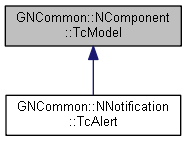
\includegraphics[width=212pt]{class_g_n_common_1_1_n_component_1_1_tc_model__inherit__graph}
\end{center}
\end{figure}


Collaboration diagram for G\+N\+Common\+:\+:N\+Component\+:\+:Tc\+Model\+:
\nopagebreak
\begin{figure}[H]
\begin{center}
\leavevmode
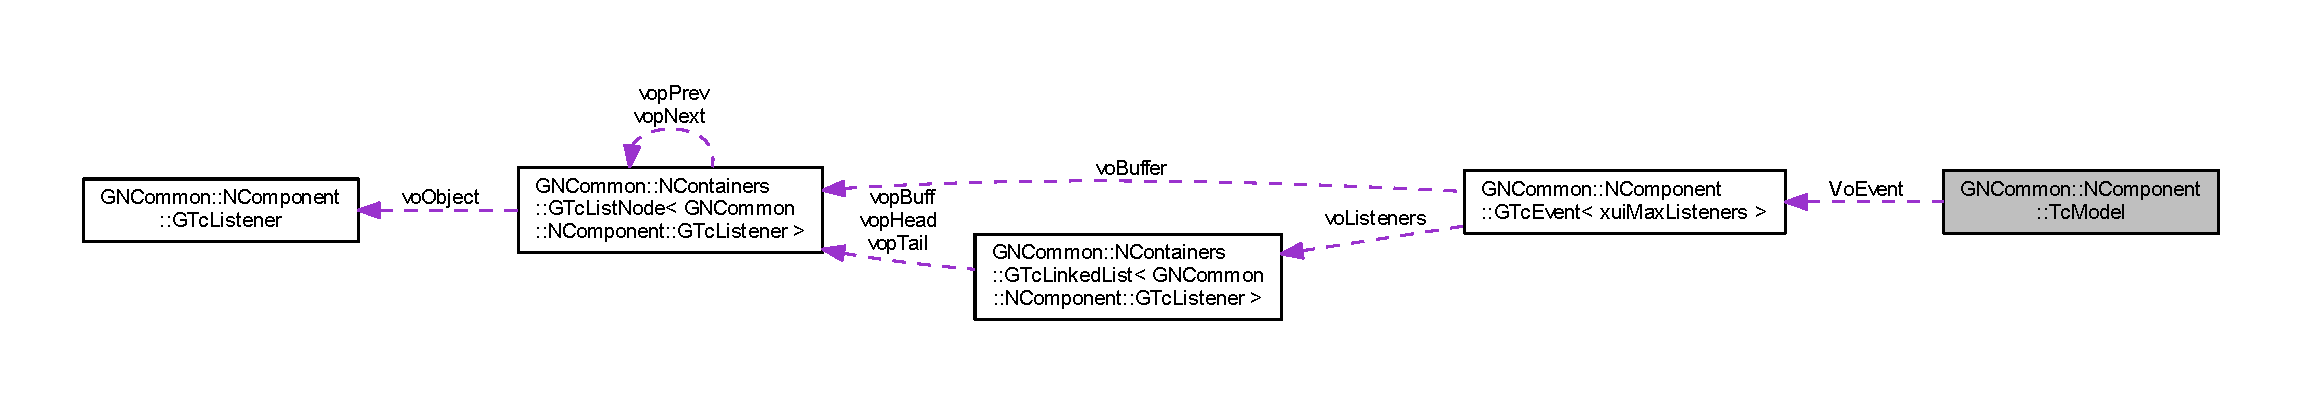
\includegraphics[width=350pt]{class_g_n_common_1_1_n_component_1_1_tc_model__coll__graph}
\end{center}
\end{figure}
\subsection*{Public Attributes}
\begin{DoxyCompactItemize}
\item 
\mbox{\Hypertarget{class_g_n_common_1_1_n_component_1_1_tc_model_ad0a33b2b2478b257ef422db8120dde41}\label{class_g_n_common_1_1_n_component_1_1_tc_model_ad0a33b2b2478b257ef422db8120dde41}} 
\mbox{\hyperlink{class_g_n_common_1_1_n_component_1_1_g_tc_event}{G\+Tc\+Event}}$<$ xui\+Max\+Listeners $>$ {\bfseries Vo\+Event}
\end{DoxyCompactItemize}
\subsection*{Static Protected Attributes}
\begin{DoxyCompactItemize}
\item 
\mbox{\Hypertarget{class_g_n_common_1_1_n_component_1_1_tc_model_a43cf22126d322790c5e15239ed00682a}\label{class_g_n_common_1_1_n_component_1_1_tc_model_a43cf22126d322790c5e15239ed00682a}} 
static const \mbox{\hyperlink{namespace_g_n_common_a941b527ef318f318aed7903dc832b7e4}{Tu32}} {\bfseries xui\+Max\+Listeners} = 16
\end{DoxyCompactItemize}


\subsection{Detailed Description}


Definition at line \mbox{\hyperlink{_model_8h_source_l00010}{10}} of file \mbox{\hyperlink{_model_8h_source}{Model.\+h}}.



The documentation for this class was generated from the following files\+:\begin{DoxyCompactItemize}
\item 
C\+:/\+Users/edwar/\+Projects/\+Bergermeister\+Home/\+Software/\+Common/inc/\+Component/Model.\+h\item 
C\+:/\+Users/edwar/\+Projects/\+Bergermeister\+Home/\+Software/\+Common/src/\+Component/Model.\+cpp\end{DoxyCompactItemize}

\hypertarget{class_g_n_common_1_1_n_notification_1_1_tc_status}{}\section{G\+N\+Common\+:\+:N\+Notification\+:\+:Tc\+Status Class Reference}
\label{class_g_n_common_1_1_n_notification_1_1_tc_status}\index{G\+N\+Common\+::\+N\+Notification\+::\+Tc\+Status@{G\+N\+Common\+::\+N\+Notification\+::\+Tc\+Status}}


{\ttfamily \#include $<$Status.\+h$>$}

\subsection*{Public Member Functions}
\begin{DoxyCompactItemize}
\item 
\mbox{\hyperlink{class_g_n_common_1_1_n_notification_1_1_tc_status_a43b5990228e5a9fbe9bfe63605f7a9d2}{Tc\+Status}} (void)
\begin{DoxyCompactList}\small\item\em Default Constructor. \end{DoxyCompactList}\item 
\mbox{\hyperlink{class_g_n_common_1_1_n_notification_1_1_tc_status_abfb0ff092f9a23017fc89dcd1d6f4e6f}{Tc\+Status}} (const \mbox{\hyperlink{class_g_n_common_1_1_n_notification_1_1_tc_status}{Tc\+Status}} \&aor\+Status)
\begin{DoxyCompactList}\small\item\em Copy Constructor. \end{DoxyCompactList}\item 
\mbox{\hyperlink{class_g_n_common_1_1_n_notification_1_1_tc_status_af14caf8abaf597904cebb6d414fd1dcf}{$\sim$\+Tc\+Status}} (void)
\begin{DoxyCompactList}\small\item\em Destructor. \end{DoxyCompactList}\item 
\mbox{\hyperlink{class_g_n_common_1_1_n_notification_1_1_tc_status}{Tc\+Status}} \& \mbox{\hyperlink{class_g_n_common_1_1_n_notification_1_1_tc_status_a97c8135ccc33bc5ba9d33f79de4ea789}{operator=}} (const \mbox{\hyperlink{class_g_n_common_1_1_n_notification_1_1_tc_status}{Tc\+Status}} \&aor\+Status)
\begin{DoxyCompactList}\small\item\em Assignment Operator. \end{DoxyCompactList}\item 
\mbox{\hyperlink{namespace_g_n_common_a8115dc7ed53b6e5b52e6bfde1632ea74}{Tb8}} \mbox{\hyperlink{class_g_n_common_1_1_n_notification_1_1_tc_status_acf4e836982c2da53ad1e6989af623c58}{operator==}} (const \mbox{\hyperlink{class_g_n_common_1_1_n_notification_1_1_tc_status}{Tc\+Status}} \&aor\+Status)
\begin{DoxyCompactList}\small\item\em Equality Operator. \end{DoxyCompactList}\item 
\mbox{\hyperlink{namespace_g_n_common_a8115dc7ed53b6e5b52e6bfde1632ea74}{Tb8}} \mbox{\hyperlink{class_g_n_common_1_1_n_notification_1_1_tc_status_acdf1eba6040e3cd5e244e21524ff0d86}{operator!=}} (const \mbox{\hyperlink{class_g_n_common_1_1_n_notification_1_1_tc_status}{Tc\+Status}} \&aor\+Status)
\begin{DoxyCompactList}\small\item\em Inequality Operator. \end{DoxyCompactList}\end{DoxyCompactItemize}
\subsection*{Public Attributes}
\begin{DoxyCompactItemize}
\item 
\mbox{\hyperlink{namespace_g_n_common_a7939e251ddbf5d3a31832dcfdc8bde39}{Tu8}} \mbox{\hyperlink{class_g_n_common_1_1_n_notification_1_1_tc_status_a69149fc8c4c5facf147993b95d171c10}{vuc\+Active}}\+: 1
\item 
\mbox{\hyperlink{namespace_g_n_common_a7939e251ddbf5d3a31832dcfdc8bde39}{Tu8}} \mbox{\hyperlink{class_g_n_common_1_1_n_notification_1_1_tc_status_a487d66407748b7a91d9d663c3fab0f2c}{vuc\+Acknowledged}}\+: 1
\item 
\mbox{\hyperlink{namespace_g_n_common_a7939e251ddbf5d3a31832dcfdc8bde39}{Tu8}} \mbox{\hyperlink{class_g_n_common_1_1_n_notification_1_1_tc_status_a36e84f5ebb3fda08f3ddaccde0a1c37b}{vuc\+Cleared}}\+: 1
\item 
\mbox{\hyperlink{namespace_g_n_common_a7939e251ddbf5d3a31832dcfdc8bde39}{Tu8}} \mbox{\hyperlink{class_g_n_common_1_1_n_notification_1_1_tc_status_a4af337a51278a09d8500bab15d929af3}{vuc\+Trigger}}\+: 1
\item 
\mbox{\hyperlink{namespace_g_n_common_a7939e251ddbf5d3a31832dcfdc8bde39}{Tu8}} \mbox{\hyperlink{class_g_n_common_1_1_n_notification_1_1_tc_status_ad8eff97b5c02e0409d3cbc65bf65c313}{vuc\+Spare1}}\+: 4
\item 
\mbox{\hyperlink{namespace_g_n_common_1_1_n_notification_a7d5c0650483fe26fa420ae5bf787566b}{Tc\+Criticality}} \mbox{\hyperlink{class_g_n_common_1_1_n_notification_1_1_tc_status_a2f8cb2528ae8cba51e3acc7f28eb2eeb}{vo\+Criticality}}
\item 
\mbox{\hyperlink{namespace_g_n_common_a7939e251ddbf5d3a31832dcfdc8bde39}{Tu8}} \mbox{\hyperlink{class_g_n_common_1_1_n_notification_1_1_tc_status_aaee139b3984634b3cc3cc7e2b7175035}{vuc\+Spare2}}
\item 
\mbox{\hyperlink{namespace_g_n_common_a7939e251ddbf5d3a31832dcfdc8bde39}{Tu8}} \mbox{\hyperlink{class_g_n_common_1_1_n_notification_1_1_tc_status_ae398de0e32d0352b0437f4267247fd6d}{vuc\+Children}}
\end{DoxyCompactItemize}


\subsection{Detailed Description}
Alert Status 

Definition at line \mbox{\hyperlink{_status_8h_source_l00015}{15}} of file \mbox{\hyperlink{_status_8h_source}{Status.\+h}}.



\subsection{Constructor \& Destructor Documentation}
\mbox{\Hypertarget{class_g_n_common_1_1_n_notification_1_1_tc_status_a43b5990228e5a9fbe9bfe63605f7a9d2}\label{class_g_n_common_1_1_n_notification_1_1_tc_status_a43b5990228e5a9fbe9bfe63605f7a9d2}} 
\index{G\+N\+Common\+::\+N\+Notification\+::\+Tc\+Status@{G\+N\+Common\+::\+N\+Notification\+::\+Tc\+Status}!Tc\+Status@{Tc\+Status}}
\index{Tc\+Status@{Tc\+Status}!G\+N\+Common\+::\+N\+Notification\+::\+Tc\+Status@{G\+N\+Common\+::\+N\+Notification\+::\+Tc\+Status}}
\subsubsection{\texorpdfstring{Tc\+Status()}{TcStatus()}\hspace{0.1cm}{\footnotesize\ttfamily [1/2]}}
{\footnotesize\ttfamily Tc\+Status\+::\+Tc\+Status (\begin{DoxyParamCaption}\item[{void}]{ }\end{DoxyParamCaption})}



Default Constructor. 

Initializes the internal members to default values.

\begin{DoxyReturn}{Returns}
None
\end{DoxyReturn}
\begin{DoxyParagraph}{Formal Parameters}

\begin{DoxyPre}{\ttfamily  None }\end{DoxyPre}

\end{DoxyParagraph}
\begin{DoxyParagraph}{Local Symbols}

\begin{DoxyPre}{\ttfamily  None }\end{DoxyPre}
 
\end{DoxyParagraph}


Definition at line \mbox{\hyperlink{_status_8cpp_source_l00025}{25}} of file \mbox{\hyperlink{_status_8cpp_source}{Status.\+cpp}}.

\mbox{\Hypertarget{class_g_n_common_1_1_n_notification_1_1_tc_status_abfb0ff092f9a23017fc89dcd1d6f4e6f}\label{class_g_n_common_1_1_n_notification_1_1_tc_status_abfb0ff092f9a23017fc89dcd1d6f4e6f}} 
\index{G\+N\+Common\+::\+N\+Notification\+::\+Tc\+Status@{G\+N\+Common\+::\+N\+Notification\+::\+Tc\+Status}!Tc\+Status@{Tc\+Status}}
\index{Tc\+Status@{Tc\+Status}!G\+N\+Common\+::\+N\+Notification\+::\+Tc\+Status@{G\+N\+Common\+::\+N\+Notification\+::\+Tc\+Status}}
\subsubsection{\texorpdfstring{Tc\+Status()}{TcStatus()}\hspace{0.1cm}{\footnotesize\ttfamily [2/2]}}
{\footnotesize\ttfamily Tc\+Status\+::\+Tc\+Status (\begin{DoxyParamCaption}\item[{const \mbox{\hyperlink{class_g_n_common_1_1_n_notification_1_1_tc_status}{Tc\+Status}} \&}]{aor\+Status }\end{DoxyParamCaption})}



Copy Constructor. 

Copies the internal members of the given Status to this Status via the assignment operator.

\begin{DoxyReturn}{Returns}
None
\end{DoxyReturn}
\begin{DoxyParagraph}{Formal Parameters}

\begin{DoxyPre}{\ttfamily [ in ]  aorStatus    Status object reference to be copied }\end{DoxyPre}

\end{DoxyParagraph}
\begin{DoxyParagraph}{Local Symbols}

\begin{DoxyPre}{\ttfamily  None }\end{DoxyPre}
 
\end{DoxyParagraph}


Definition at line \mbox{\hyperlink{_status_8cpp_source_l00050}{50}} of file \mbox{\hyperlink{_status_8cpp_source}{Status.\+cpp}}.

\mbox{\Hypertarget{class_g_n_common_1_1_n_notification_1_1_tc_status_af14caf8abaf597904cebb6d414fd1dcf}\label{class_g_n_common_1_1_n_notification_1_1_tc_status_af14caf8abaf597904cebb6d414fd1dcf}} 
\index{G\+N\+Common\+::\+N\+Notification\+::\+Tc\+Status@{G\+N\+Common\+::\+N\+Notification\+::\+Tc\+Status}!````~Tc\+Status@{$\sim$\+Tc\+Status}}
\index{````~Tc\+Status@{$\sim$\+Tc\+Status}!G\+N\+Common\+::\+N\+Notification\+::\+Tc\+Status@{G\+N\+Common\+::\+N\+Notification\+::\+Tc\+Status}}
\subsubsection{\texorpdfstring{$\sim$\+Tc\+Status()}{~TcStatus()}}
{\footnotesize\ttfamily Tc\+Status\+::$\sim$\+Tc\+Status (\begin{DoxyParamCaption}\item[{void}]{ }\end{DoxyParamCaption})}



Destructor. 

Nothing to destruct

\begin{DoxyReturn}{Returns}
None
\end{DoxyReturn}
\begin{DoxyParagraph}{Formal Parameters}

\begin{DoxyPre}{\ttfamily  None }\end{DoxyPre}

\end{DoxyParagraph}
\begin{DoxyParagraph}{Local Symbols}

\begin{DoxyPre}{\ttfamily  None }\end{DoxyPre}
 
\end{DoxyParagraph}


Definition at line \mbox{\hyperlink{_status_8cpp_source_l00068}{68}} of file \mbox{\hyperlink{_status_8cpp_source}{Status.\+cpp}}.



\subsection{Member Function Documentation}
\mbox{\Hypertarget{class_g_n_common_1_1_n_notification_1_1_tc_status_acdf1eba6040e3cd5e244e21524ff0d86}\label{class_g_n_common_1_1_n_notification_1_1_tc_status_acdf1eba6040e3cd5e244e21524ff0d86}} 
\index{G\+N\+Common\+::\+N\+Notification\+::\+Tc\+Status@{G\+N\+Common\+::\+N\+Notification\+::\+Tc\+Status}!operator"!=@{operator"!=}}
\index{operator"!=@{operator"!=}!G\+N\+Common\+::\+N\+Notification\+::\+Tc\+Status@{G\+N\+Common\+::\+N\+Notification\+::\+Tc\+Status}}
\subsubsection{\texorpdfstring{operator"!=()}{operator!=()}}
{\footnotesize\ttfamily \mbox{\hyperlink{namespace_g_n_common_a8115dc7ed53b6e5b52e6bfde1632ea74}{Tb8}} Tc\+Status\+::operator!= (\begin{DoxyParamCaption}\item[{const \mbox{\hyperlink{class_g_n_common_1_1_n_notification_1_1_tc_status}{Tc\+Status}} \&}]{aor\+Status }\end{DoxyParamCaption})}



Inequality Operator. 

Compares this Status to the given Status and returns if they are not equal.

\begin{DoxyReturn}{Returns}
True if any of this Status\textquotesingle{}s internal members are not equal to the given Status\textquotesingle{}s internal members
\end{DoxyReturn}
\begin{DoxyParagraph}{Formal Parameters}

\begin{DoxyPre}{\ttfamily [ in ]  aorStatus    Status object reference to be compared }\end{DoxyPre}

\end{DoxyParagraph}
\begin{DoxyParagraph}{Local Symbols}

\begin{DoxyPre}{\ttfamily  None }\end{DoxyPre}
 
\end{DoxyParagraph}


Definition at line \mbox{\hyperlink{_status_8cpp_source_l00146}{146}} of file \mbox{\hyperlink{_status_8cpp_source}{Status.\+cpp}}.

\mbox{\Hypertarget{class_g_n_common_1_1_n_notification_1_1_tc_status_a97c8135ccc33bc5ba9d33f79de4ea789}\label{class_g_n_common_1_1_n_notification_1_1_tc_status_a97c8135ccc33bc5ba9d33f79de4ea789}} 
\index{G\+N\+Common\+::\+N\+Notification\+::\+Tc\+Status@{G\+N\+Common\+::\+N\+Notification\+::\+Tc\+Status}!operator=@{operator=}}
\index{operator=@{operator=}!G\+N\+Common\+::\+N\+Notification\+::\+Tc\+Status@{G\+N\+Common\+::\+N\+Notification\+::\+Tc\+Status}}
\subsubsection{\texorpdfstring{operator=()}{operator=()}}
{\footnotesize\ttfamily \mbox{\hyperlink{class_g_n_common_1_1_n_notification_1_1_tc_status}{Tc\+Status}} \& Tc\+Status\+::operator= (\begin{DoxyParamCaption}\item[{const \mbox{\hyperlink{class_g_n_common_1_1_n_notification_1_1_tc_status}{Tc\+Status}} \&}]{aor\+Status }\end{DoxyParamCaption})}



Assignment Operator. 

Copies the internal members of the given Status

\begin{DoxyReturn}{Returns}
Status object reference to this Status
\end{DoxyReturn}
\begin{DoxyParagraph}{Formal Parameters}

\begin{DoxyPre}{\ttfamily [ in ]  aorStatus    Status object reference to be copied }\end{DoxyPre}

\end{DoxyParagraph}
\begin{DoxyParagraph}{Local Symbols}

\begin{DoxyPre}{\ttfamily  None }\end{DoxyPre}
 
\end{DoxyParagraph}


Definition at line \mbox{\hyperlink{_status_8cpp_source_l00087}{87}} of file \mbox{\hyperlink{_status_8cpp_source}{Status.\+cpp}}.

\mbox{\Hypertarget{class_g_n_common_1_1_n_notification_1_1_tc_status_acf4e836982c2da53ad1e6989af623c58}\label{class_g_n_common_1_1_n_notification_1_1_tc_status_acf4e836982c2da53ad1e6989af623c58}} 
\index{G\+N\+Common\+::\+N\+Notification\+::\+Tc\+Status@{G\+N\+Common\+::\+N\+Notification\+::\+Tc\+Status}!operator==@{operator==}}
\index{operator==@{operator==}!G\+N\+Common\+::\+N\+Notification\+::\+Tc\+Status@{G\+N\+Common\+::\+N\+Notification\+::\+Tc\+Status}}
\subsubsection{\texorpdfstring{operator==()}{operator==()}}
{\footnotesize\ttfamily \mbox{\hyperlink{namespace_g_n_common_a8115dc7ed53b6e5b52e6bfde1632ea74}{Tb8}} Tc\+Status\+::operator== (\begin{DoxyParamCaption}\item[{const \mbox{\hyperlink{class_g_n_common_1_1_n_notification_1_1_tc_status}{Tc\+Status}} \&}]{aor\+Status }\end{DoxyParamCaption})}



Equality Operator. 

Compares this Status to the given Status and returns if they are equal.

\begin{DoxyReturn}{Returns}
True if all of this Status\textquotesingle{}s internal members equal the given Status\textquotesingle{}s internal members
\end{DoxyReturn}
\begin{DoxyParagraph}{Formal Parameters}

\begin{DoxyPre}{\ttfamily [ in ]  aorStatus    Status object reference to be compared }\end{DoxyPre}

\end{DoxyParagraph}
\begin{DoxyParagraph}{Local Symbols}

\begin{DoxyPre}{\ttfamily  kbEqual    Flag indicating if the Statuses are equal }\end{DoxyPre}
 
\end{DoxyParagraph}


Definition at line \mbox{\hyperlink{_status_8cpp_source_l00114}{114}} of file \mbox{\hyperlink{_status_8cpp_source}{Status.\+cpp}}.



\subsection{Member Data Documentation}
\mbox{\Hypertarget{class_g_n_common_1_1_n_notification_1_1_tc_status_a2f8cb2528ae8cba51e3acc7f28eb2eeb}\label{class_g_n_common_1_1_n_notification_1_1_tc_status_a2f8cb2528ae8cba51e3acc7f28eb2eeb}} 
\index{G\+N\+Common\+::\+N\+Notification\+::\+Tc\+Status@{G\+N\+Common\+::\+N\+Notification\+::\+Tc\+Status}!vo\+Criticality@{vo\+Criticality}}
\index{vo\+Criticality@{vo\+Criticality}!G\+N\+Common\+::\+N\+Notification\+::\+Tc\+Status@{G\+N\+Common\+::\+N\+Notification\+::\+Tc\+Status}}
\subsubsection{\texorpdfstring{vo\+Criticality}{voCriticality}}
{\footnotesize\ttfamily \mbox{\hyperlink{namespace_g_n_common_1_1_n_notification_a7d5c0650483fe26fa420ae5bf787566b}{Tc\+Criticality}} G\+N\+Common\+::\+N\+Notification\+::\+Tc\+Status\+::vo\+Criticality}

Bits 8 -\/ 15 \+: Alert Level 

Definition at line \mbox{\hyperlink{_status_8h_source_l00023}{23}} of file \mbox{\hyperlink{_status_8h_source}{Status.\+h}}.

\mbox{\Hypertarget{class_g_n_common_1_1_n_notification_1_1_tc_status_a487d66407748b7a91d9d663c3fab0f2c}\label{class_g_n_common_1_1_n_notification_1_1_tc_status_a487d66407748b7a91d9d663c3fab0f2c}} 
\index{G\+N\+Common\+::\+N\+Notification\+::\+Tc\+Status@{G\+N\+Common\+::\+N\+Notification\+::\+Tc\+Status}!vuc\+Acknowledged@{vuc\+Acknowledged}}
\index{vuc\+Acknowledged@{vuc\+Acknowledged}!G\+N\+Common\+::\+N\+Notification\+::\+Tc\+Status@{G\+N\+Common\+::\+N\+Notification\+::\+Tc\+Status}}
\subsubsection{\texorpdfstring{vuc\+Acknowledged}{vucAcknowledged}}
{\footnotesize\ttfamily \mbox{\hyperlink{namespace_g_n_common_a7939e251ddbf5d3a31832dcfdc8bde39}{Tu8}} G\+N\+Common\+::\+N\+Notification\+::\+Tc\+Status\+::vuc\+Acknowledged}

Bit 1 \+: Acknowledged Flag 

Definition at line \mbox{\hyperlink{_status_8h_source_l00019}{19}} of file \mbox{\hyperlink{_status_8h_source}{Status.\+h}}.

\mbox{\Hypertarget{class_g_n_common_1_1_n_notification_1_1_tc_status_a69149fc8c4c5facf147993b95d171c10}\label{class_g_n_common_1_1_n_notification_1_1_tc_status_a69149fc8c4c5facf147993b95d171c10}} 
\index{G\+N\+Common\+::\+N\+Notification\+::\+Tc\+Status@{G\+N\+Common\+::\+N\+Notification\+::\+Tc\+Status}!vuc\+Active@{vuc\+Active}}
\index{vuc\+Active@{vuc\+Active}!G\+N\+Common\+::\+N\+Notification\+::\+Tc\+Status@{G\+N\+Common\+::\+N\+Notification\+::\+Tc\+Status}}
\subsubsection{\texorpdfstring{vuc\+Active}{vucActive}}
{\footnotesize\ttfamily \mbox{\hyperlink{namespace_g_n_common_a7939e251ddbf5d3a31832dcfdc8bde39}{Tu8}} G\+N\+Common\+::\+N\+Notification\+::\+Tc\+Status\+::vuc\+Active}

Bit 0 \+: Active Flag 

Definition at line \mbox{\hyperlink{_status_8h_source_l00018}{18}} of file \mbox{\hyperlink{_status_8h_source}{Status.\+h}}.

\mbox{\Hypertarget{class_g_n_common_1_1_n_notification_1_1_tc_status_ae398de0e32d0352b0437f4267247fd6d}\label{class_g_n_common_1_1_n_notification_1_1_tc_status_ae398de0e32d0352b0437f4267247fd6d}} 
\index{G\+N\+Common\+::\+N\+Notification\+::\+Tc\+Status@{G\+N\+Common\+::\+N\+Notification\+::\+Tc\+Status}!vuc\+Children@{vuc\+Children}}
\index{vuc\+Children@{vuc\+Children}!G\+N\+Common\+::\+N\+Notification\+::\+Tc\+Status@{G\+N\+Common\+::\+N\+Notification\+::\+Tc\+Status}}
\subsubsection{\texorpdfstring{vuc\+Children}{vucChildren}}
{\footnotesize\ttfamily \mbox{\hyperlink{namespace_g_n_common_a7939e251ddbf5d3a31832dcfdc8bde39}{Tu8}} G\+N\+Common\+::\+N\+Notification\+::\+Tc\+Status\+::vuc\+Children}

Bits 24 -\/ 31 \+: Number of Child Alerts 

Definition at line \mbox{\hyperlink{_status_8h_source_l00025}{25}} of file \mbox{\hyperlink{_status_8h_source}{Status.\+h}}.

\mbox{\Hypertarget{class_g_n_common_1_1_n_notification_1_1_tc_status_a36e84f5ebb3fda08f3ddaccde0a1c37b}\label{class_g_n_common_1_1_n_notification_1_1_tc_status_a36e84f5ebb3fda08f3ddaccde0a1c37b}} 
\index{G\+N\+Common\+::\+N\+Notification\+::\+Tc\+Status@{G\+N\+Common\+::\+N\+Notification\+::\+Tc\+Status}!vuc\+Cleared@{vuc\+Cleared}}
\index{vuc\+Cleared@{vuc\+Cleared}!G\+N\+Common\+::\+N\+Notification\+::\+Tc\+Status@{G\+N\+Common\+::\+N\+Notification\+::\+Tc\+Status}}
\subsubsection{\texorpdfstring{vuc\+Cleared}{vucCleared}}
{\footnotesize\ttfamily \mbox{\hyperlink{namespace_g_n_common_a7939e251ddbf5d3a31832dcfdc8bde39}{Tu8}} G\+N\+Common\+::\+N\+Notification\+::\+Tc\+Status\+::vuc\+Cleared}

Bit 2 \+: Cleared Flag 

Definition at line \mbox{\hyperlink{_status_8h_source_l00020}{20}} of file \mbox{\hyperlink{_status_8h_source}{Status.\+h}}.

\mbox{\Hypertarget{class_g_n_common_1_1_n_notification_1_1_tc_status_ad8eff97b5c02e0409d3cbc65bf65c313}\label{class_g_n_common_1_1_n_notification_1_1_tc_status_ad8eff97b5c02e0409d3cbc65bf65c313}} 
\index{G\+N\+Common\+::\+N\+Notification\+::\+Tc\+Status@{G\+N\+Common\+::\+N\+Notification\+::\+Tc\+Status}!vuc\+Spare1@{vuc\+Spare1}}
\index{vuc\+Spare1@{vuc\+Spare1}!G\+N\+Common\+::\+N\+Notification\+::\+Tc\+Status@{G\+N\+Common\+::\+N\+Notification\+::\+Tc\+Status}}
\subsubsection{\texorpdfstring{vuc\+Spare1}{vucSpare1}}
{\footnotesize\ttfamily \mbox{\hyperlink{namespace_g_n_common_a7939e251ddbf5d3a31832dcfdc8bde39}{Tu8}} G\+N\+Common\+::\+N\+Notification\+::\+Tc\+Status\+::vuc\+Spare1}

Bits 4 -\/ 7 \+: Spare Flags 

Definition at line \mbox{\hyperlink{_status_8h_source_l00022}{22}} of file \mbox{\hyperlink{_status_8h_source}{Status.\+h}}.

\mbox{\Hypertarget{class_g_n_common_1_1_n_notification_1_1_tc_status_aaee139b3984634b3cc3cc7e2b7175035}\label{class_g_n_common_1_1_n_notification_1_1_tc_status_aaee139b3984634b3cc3cc7e2b7175035}} 
\index{G\+N\+Common\+::\+N\+Notification\+::\+Tc\+Status@{G\+N\+Common\+::\+N\+Notification\+::\+Tc\+Status}!vuc\+Spare2@{vuc\+Spare2}}
\index{vuc\+Spare2@{vuc\+Spare2}!G\+N\+Common\+::\+N\+Notification\+::\+Tc\+Status@{G\+N\+Common\+::\+N\+Notification\+::\+Tc\+Status}}
\subsubsection{\texorpdfstring{vuc\+Spare2}{vucSpare2}}
{\footnotesize\ttfamily \mbox{\hyperlink{namespace_g_n_common_a7939e251ddbf5d3a31832dcfdc8bde39}{Tu8}} G\+N\+Common\+::\+N\+Notification\+::\+Tc\+Status\+::vuc\+Spare2}

Bits 16 -\/ 23 \+: Spare 

Definition at line \mbox{\hyperlink{_status_8h_source_l00024}{24}} of file \mbox{\hyperlink{_status_8h_source}{Status.\+h}}.

\mbox{\Hypertarget{class_g_n_common_1_1_n_notification_1_1_tc_status_a4af337a51278a09d8500bab15d929af3}\label{class_g_n_common_1_1_n_notification_1_1_tc_status_a4af337a51278a09d8500bab15d929af3}} 
\index{G\+N\+Common\+::\+N\+Notification\+::\+Tc\+Status@{G\+N\+Common\+::\+N\+Notification\+::\+Tc\+Status}!vuc\+Trigger@{vuc\+Trigger}}
\index{vuc\+Trigger@{vuc\+Trigger}!G\+N\+Common\+::\+N\+Notification\+::\+Tc\+Status@{G\+N\+Common\+::\+N\+Notification\+::\+Tc\+Status}}
\subsubsection{\texorpdfstring{vuc\+Trigger}{vucTrigger}}
{\footnotesize\ttfamily \mbox{\hyperlink{namespace_g_n_common_a7939e251ddbf5d3a31832dcfdc8bde39}{Tu8}} G\+N\+Common\+::\+N\+Notification\+::\+Tc\+Status\+::vuc\+Trigger}

Bit 3 \+: Trigger Available Flag 

Definition at line \mbox{\hyperlink{_status_8h_source_l00021}{21}} of file \mbox{\hyperlink{_status_8h_source}{Status.\+h}}.



The documentation for this class was generated from the following files\+:\begin{DoxyCompactItemize}
\item 
C\+:/\+Projects/\+Bergermeister\+Home/\+Software/\+Common/inc/\+Notification/\mbox{\hyperlink{_status_8h}{Status.\+h}}\item 
C\+:/\+Projects/\+Bergermeister\+Home/\+Software/\+Common/src/\+Notification/\mbox{\hyperlink{_status_8cpp}{Status.\+cpp}}\end{DoxyCompactItemize}

\chapter{File Documentation}
\hypertarget{_c_r_c32_8h}{}\section{C\+:/\+Projects/\+Bergermeister\+Home/\+Software/\+Common/inc/\+Data\+Authentication/\+C\+R\+C32.h File Reference}
\label{_c_r_c32_8h}\index{C\+:/\+Projects/\+Bergermeister\+Home/\+Software/\+Common/inc/\+Data\+Authentication/\+C\+R\+C32.\+h@{C\+:/\+Projects/\+Bergermeister\+Home/\+Software/\+Common/inc/\+Data\+Authentication/\+C\+R\+C32.\+h}}


Package interface for the C\+R\+C32 class.  


{\ttfamily \#include $<$Types.\+h$>$}\newline
\subsection*{Classes}
\begin{DoxyCompactItemize}
\item 
class \mbox{\hyperlink{class_g_n_common_1_1_n_data_authentication_1_1_tc_c_r_c32}{G\+N\+Common\+::\+N\+Data\+Authentication\+::\+Tc\+C\+R\+C32}}
\end{DoxyCompactItemize}
\subsection*{Namespaces}
\begin{DoxyCompactItemize}
\item 
 \mbox{\hyperlink{namespace_g_n_common}{G\+N\+Common}}
\begin{DoxyCompactList}\small\item\em Namespace containing Common components and infrastrucutre. \end{DoxyCompactList}\item 
 \mbox{\hyperlink{namespace_g_n_common_1_1_n_data_authentication}{G\+N\+Common\+::\+N\+Data\+Authentication}}
\begin{DoxyCompactList}\small\item\em Namespace containing Data Authentication and Validity Checking utilities. \end{DoxyCompactList}\end{DoxyCompactItemize}


\subsection{Detailed Description}
Package interface for the C\+R\+C32 class. 



Definition in file \mbox{\hyperlink{_c_r_c32_8h_source}{C\+R\+C32.\+h}}.


\hypertarget{_c_r_c32_8h_source}{}\section{C\+R\+C32.\+h}
\label{_c_r_c32_8h_source}\index{C\+:/\+Projects/\+Bergermeister\+Home/\+Software/\+Common/inc/\+Data\+Authentication/\+C\+R\+C32.\+h@{C\+:/\+Projects/\+Bergermeister\+Home/\+Software/\+Common/inc/\+Data\+Authentication/\+C\+R\+C32.\+h}}

\begin{DoxyCode}
00001 
00005 \textcolor{preprocessor}{#pragma once}
00006 
00007 \textcolor{preprocessor}{#include <\mbox{\hyperlink{_types_8h}{Types.h}}>}
00008 
00009 \textcolor{keyword}{namespace }\mbox{\hyperlink{namespace_g_n_common}{GNCommon}}
00010 \{
\Hypertarget{_c_r_c32_8h_source_l00012}\mbox{\hyperlink{namespace_g_n_common_1_1_n_data_authentication}{00012}}    \textcolor{keyword}{namespace }NDataAuthentication
00013    \{
\Hypertarget{_c_r_c32_8h_source_l00014}\mbox{\hyperlink{class_g_n_common_1_1_n_data_authentication_1_1_tc_c_r_c32}{00014}}       \textcolor{keyword}{class }\mbox{\hyperlink{class_g_n_common_1_1_n_data_authentication_1_1_tc_c_r_c32}{TcCRC32}}
00015       \{
00016       \textcolor{keyword}{protected}:     \textcolor{comment}{// Protected Attributes}
00017          \textcolor{keyword}{static} \textcolor{keyword}{const} \mbox{\hyperlink{namespace_g_n_common_a941b527ef318f318aed7903dc832b7e4}{Tu32}} xuiDefaultSeed = 0xFFFFFFFF;
00018          \textcolor{keyword}{static} \textcolor{keyword}{const} \mbox{\hyperlink{namespace_g_n_common_a941b527ef318f318aed7903dc832b7e4}{Tu32}} xuiTableCRC    = 0x6FCF9E13;
00019          \textcolor{keyword}{static} \textcolor{keyword}{const} \mbox{\hyperlink{namespace_g_n_common_a941b527ef318f318aed7903dc832b7e4}{Tu32}} xuiShift8      = 8;
00020          \textcolor{keyword}{static} \textcolor{keyword}{const} \mbox{\hyperlink{namespace_g_n_common_a941b527ef318f318aed7903dc832b7e4}{Tu32}} xuiMaskByte    = 0x000000FF;
00021          \textcolor{keyword}{static} \textcolor{keyword}{const} \mbox{\hyperlink{namespace_g_n_common_a941b527ef318f318aed7903dc832b7e4}{Tu32}} xuiMaskAlign   = 0x00000003;
00022          \textcolor{keyword}{static} \textcolor{keyword}{const} \mbox{\hyperlink{namespace_g_n_common_a941b527ef318f318aed7903dc832b7e4}{Tu32}} xuiTableSize   = 256;
\Hypertarget{_c_r_c32_8h_source_l00023}\mbox{\hyperlink{class_g_n_common_1_1_n_data_authentication_1_1_tc_c_r_c32_a2c841dc8051fc7e1719224929f24b32d}{00023}}          \textcolor{keyword}{static} \textcolor{keyword}{const} \mbox{\hyperlink{namespace_g_n_common_a941b527ef318f318aed7903dc832b7e4}{Tu32}} \mbox{\hyperlink{class_g_n_common_1_1_n_data_authentication_1_1_tc_c_r_c32_a2c841dc8051fc7e1719224929f24b32d}{xuiTable}}[ xuiTableSize ];
00024       
00025       \textcolor{keyword}{public}:        \textcolor{comment}{// Public Methods}
00026          \mbox{\hyperlink{class_g_n_common_1_1_n_data_authentication_1_1_tc_c_r_c32}{TcCRC32}}( \textcolor{keywordtype}{void} );
00027 
00028          \mbox{\hyperlink{namespace_g_n_common_a941b527ef318f318aed7903dc832b7e4}{Tu32}} MGet( \textcolor{keyword}{const} \mbox{\hyperlink{namespace_g_n_common_a7939e251ddbf5d3a31832dcfdc8bde39}{Tu8}}* aucpBuffer, \textcolor{keyword}{const} \mbox{\hyperlink{namespace_g_n_common_a941b527ef318f318aed7903dc832b7e4}{Tu32}} auiBytes, \textcolor{keyword}{const} 
      \mbox{\hyperlink{namespace_g_n_common_a941b527ef318f318aed7903dc832b7e4}{Tu32}} auiSeed = xuiDefaultSeed ) \textcolor{keyword}{const};
00029 
00030          \mbox{\hyperlink{namespace_g_n_common_a8115dc7ed53b6e5b52e6bfde1632ea74}{Tb8}} MVerify( \textcolor{keywordtype}{void} ) \textcolor{keyword}{const};
00031 
00032       \textcolor{keyword}{protected}:     \textcolor{comment}{// Protected Methods}
00033          \mbox{\hyperlink{namespace_g_n_common_a941b527ef318f318aed7903dc832b7e4}{Tu32}} mGetLE( \textcolor{keyword}{const} \mbox{\hyperlink{namespace_g_n_common_a7939e251ddbf5d3a31832dcfdc8bde39}{Tu8}}* aucpBuffer, \textcolor{keyword}{const} \mbox{\hyperlink{namespace_g_n_common_a941b527ef318f318aed7903dc832b7e4}{Tu32}} auiBytes, \textcolor{keyword}{const} 
      \mbox{\hyperlink{namespace_g_n_common_a941b527ef318f318aed7903dc832b7e4}{Tu32}} auiSeed = xuiDefaultSeed ) \textcolor{keyword}{const};
00034          \mbox{\hyperlink{namespace_g_n_common_a941b527ef318f318aed7903dc832b7e4}{Tu32}} mGetBE( \textcolor{keyword}{const} \mbox{\hyperlink{namespace_g_n_common_a7939e251ddbf5d3a31832dcfdc8bde39}{Tu8}}* aucpBuffer, \textcolor{keyword}{const} \mbox{\hyperlink{namespace_g_n_common_a941b527ef318f318aed7903dc832b7e4}{Tu32}} auiBytes, \textcolor{keyword}{const} 
      \mbox{\hyperlink{namespace_g_n_common_a941b527ef318f318aed7903dc832b7e4}{Tu32}} auiSeed = xuiDefaultSeed ) \textcolor{keyword}{const};
00035       \};
00036    \}
00037 \}
\end{DoxyCode}

\hypertarget{_alert_8h}{}\section{C\+:/\+Users/edwar/\+Projects/\+Bergermeister\+Home/\+Software/\+Common/inc/\+Notification/\+Alert.h File Reference}
\label{_alert_8h}\index{C\+:/\+Users/edwar/\+Projects/\+Bergermeister\+Home/\+Software/\+Common/inc/\+Notification/\+Alert.\+h@{C\+:/\+Users/edwar/\+Projects/\+Bergermeister\+Home/\+Software/\+Common/inc/\+Notification/\+Alert.\+h}}


Package interface for the Alert Class.  


{\ttfamily \#include $<$Types.\+h$>$}\newline
{\ttfamily \#include $<$Component\textbackslash{}\+Model.\+h$>$}\newline
{\ttfamily \#include $<$Notification\textbackslash{}\+Component\+Id.\+h$>$}\newline
{\ttfamily \#include $<$Notification\textbackslash{}\+Identifier.\+h$>$}\newline
{\ttfamily \#include $<$Notification\textbackslash{}\+Status.\+h$>$}\newline
Include dependency graph for Alert.\+h\+:
\nopagebreak
\begin{figure}[H]
\begin{center}
\leavevmode
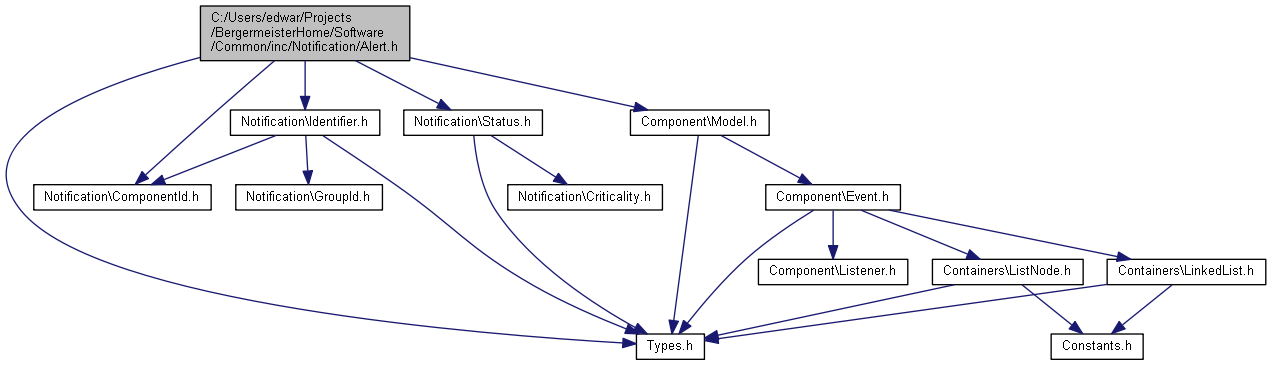
\includegraphics[width=350pt]{_alert_8h__incl}
\end{center}
\end{figure}
This graph shows which files directly or indirectly include this file\+:
\nopagebreak
\begin{figure}[H]
\begin{center}
\leavevmode
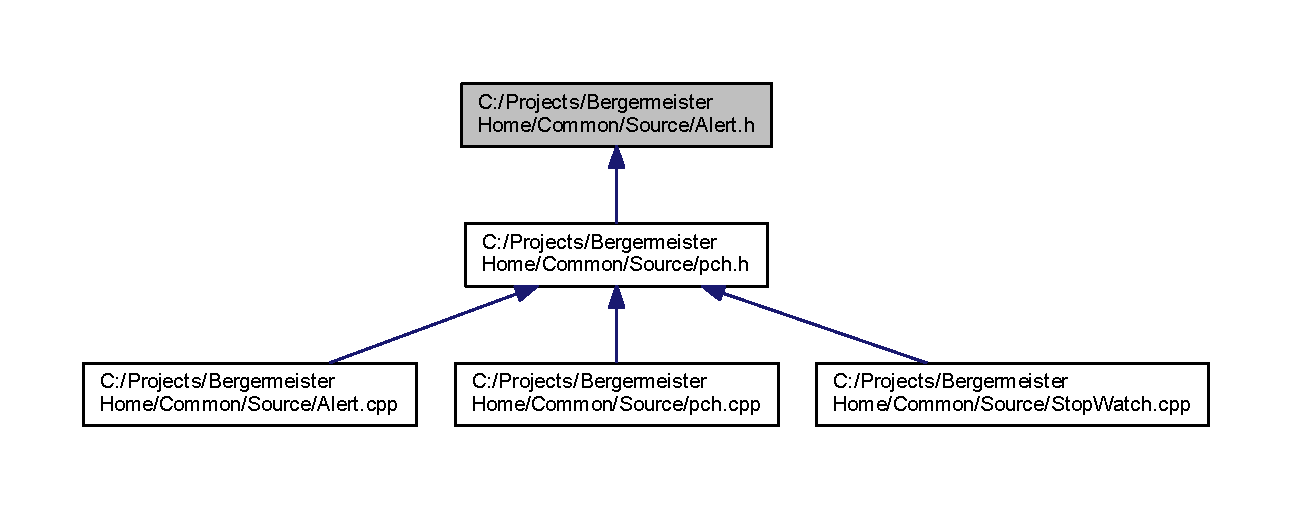
\includegraphics[width=248pt]{_alert_8h__dep__incl}
\end{center}
\end{figure}
\subsection*{Classes}
\begin{DoxyCompactItemize}
\item 
class \mbox{\hyperlink{class_g_n_common_1_1_n_notification_1_1_tc_alert}{G\+N\+Common\+::\+N\+Notification\+::\+Tc\+Alert}}
\end{DoxyCompactItemize}
\subsection*{Namespaces}
\begin{DoxyCompactItemize}
\item 
 \mbox{\hyperlink{namespace_g_n_common}{G\+N\+Common}}
\begin{DoxyCompactList}\small\item\em Namespace containing Common components and infrastrucutre. \end{DoxyCompactList}\item 
 \mbox{\hyperlink{namespace_g_n_common_1_1_n_notification}{G\+N\+Common\+::\+N\+Notification}}
\begin{DoxyCompactList}\small\item\em Namespace containing system Alerts. \end{DoxyCompactList}\end{DoxyCompactItemize}


\subsection{Detailed Description}
Package interface for the Alert Class. 



Definition in file \mbox{\hyperlink{_alert_8h_source}{Alert.\+h}}.


\hypertarget{_alert_8h_source}{}\section{Alert.\+h}
\label{_alert_8h_source}\index{C\+:/\+Users/edwar/\+Projects/\+Bergermeister\+Home/\+Software/\+Common/inc/\+Notification/\+Alert.\+h@{C\+:/\+Users/edwar/\+Projects/\+Bergermeister\+Home/\+Software/\+Common/inc/\+Notification/\+Alert.\+h}}

\begin{DoxyCode}
00001 
00005 \textcolor{preprocessor}{#pragma once}
00006 
00007 \textcolor{preprocessor}{#include <\mbox{\hyperlink{_types_8h}{Types.h}}>}
00008 \textcolor{preprocessor}{#include <Component\(\backslash\)Model.h>}
00009 \textcolor{preprocessor}{#include <\mbox{\hyperlink{_component_id_8h}{Notification\(\backslash\)ComponentId.h}}>}
00010 \textcolor{preprocessor}{#include <\mbox{\hyperlink{_identifier_8h}{Notification\(\backslash\)Identifier.h}}>}
00011 \textcolor{preprocessor}{#include <\mbox{\hyperlink{_status_8h}{Notification\(\backslash\)Status.h}}>}
00012 
00013 \textcolor{keyword}{namespace }\mbox{\hyperlink{namespace_g_n_common}{GNCommon}}
00014 \{
\Hypertarget{_alert_8h_source_l00016}\mbox{\hyperlink{namespace_g_n_common_1_1_n_notification}{00016}}    \textcolor{keyword}{namespace }NNotification
00017    \{
\Hypertarget{_alert_8h_source_l00019}\mbox{\hyperlink{class_g_n_common_1_1_n_notification_1_1_tc_alert}{00019}}       \textcolor{keyword}{class }\mbox{\hyperlink{class_g_n_common_1_1_n_notification_1_1_tc_alert}{TcAlert}} : \textcolor{keyword}{public} \mbox{\hyperlink{class_g_n_common_1_1_n_component_1_1_tc_model}{GNCommon::NComponent::TcModel}}
00020       \{
00021       \textcolor{keyword}{public}:        \textcolor{comment}{// Public Type Definitions}
\Hypertarget{_alert_8h_source_l00022}\mbox{\hyperlink{class_g_n_common_1_1_n_notification_1_1_tc_alert_a44f63050a2f1c7a4876a31ce2ffd2d06}{00022}}          \textcolor{keyword}{static} \textcolor{keyword}{const} \mbox{\hyperlink{namespace_g_n_common_a941b527ef318f318aed7903dc832b7e4}{Tu32}} \mbox{\hyperlink{class_g_n_common_1_1_n_notification_1_1_tc_alert_a44f63050a2f1c7a4876a31ce2ffd2d06}{XuiSizeOfIdentifier}} = \textcolor{keyword}{sizeof}( 
      \mbox{\hyperlink{class_g_n_common_1_1_n_notification_1_1_tc_identifier}{TcIdentifier}} ); 
\Hypertarget{_alert_8h_source_l00023}\mbox{\hyperlink{class_g_n_common_1_1_n_notification_1_1_tc_alert_a59f856e0a33731ee0c235271bb013a34}{00023}}          \textcolor{keyword}{static} \textcolor{keyword}{const} \mbox{\hyperlink{namespace_g_n_common_a941b527ef318f318aed7903dc832b7e4}{Tu32}} \mbox{\hyperlink{class_g_n_common_1_1_n_notification_1_1_tc_alert_a59f856e0a33731ee0c235271bb013a34}{XuiSizeOfStatus}}     = \textcolor{keyword}{sizeof}( 
      \mbox{\hyperlink{class_g_n_common_1_1_n_notification_1_1_tc_status}{TcStatus}}     ); 
00025       \textcolor{keyword}{protected}:     \textcolor{comment}{// Protected Attributes}
\Hypertarget{_alert_8h_source_l00026}\mbox{\hyperlink{class_g_n_common_1_1_n_notification_1_1_tc_alert_aa42573703fd6fa2ba90aa010fdc659ca}{00026}}          \mbox{\hyperlink{class_g_n_common_1_1_n_notification_1_1_tc_identifier}{TcIdentifier}} \mbox{\hyperlink{class_g_n_common_1_1_n_notification_1_1_tc_alert_aa42573703fd6fa2ba90aa010fdc659ca}{voID}};         
\Hypertarget{_alert_8h_source_l00027}\mbox{\hyperlink{class_g_n_common_1_1_n_notification_1_1_tc_alert_ae993e1ea34de5347b08b21c9264cdb8e}{00027}}          \mbox{\hyperlink{class_g_n_common_1_1_n_notification_1_1_tc_status}{TcStatus}}     \mbox{\hyperlink{class_g_n_common_1_1_n_notification_1_1_tc_alert_ae993e1ea34de5347b08b21c9264cdb8e}{voStatus}};     
\Hypertarget{_alert_8h_source_l00028}\mbox{\hyperlink{class_g_n_common_1_1_n_notification_1_1_tc_alert_a3c6f656e3e526b9f97942188d7bb2930}{00028}}          \mbox{\hyperlink{namespace_g_n_common_a9404ee6090c788ae70aebd1436ceb97d}{Tu64}}         \mbox{\hyperlink{class_g_n_common_1_1_n_notification_1_1_tc_alert_a3c6f656e3e526b9f97942188d7bb2930}{vulTimestamp}}; 
\Hypertarget{_alert_8h_source_l00029}\mbox{\hyperlink{class_g_n_common_1_1_n_notification_1_1_tc_alert_ab49cb616a0e61e74234264d775a3408a}{00029}}          \mbox{\hyperlink{namespace_g_n_common_a9404ee6090c788ae70aebd1436ceb97d}{Tu64}}         \mbox{\hyperlink{class_g_n_common_1_1_n_notification_1_1_tc_alert_ab49cb616a0e61e74234264d775a3408a}{vulData}};      
00031       \textcolor{keyword}{public}:        \textcolor{comment}{// Public Methods}
00032          \mbox{\hyperlink{class_g_n_common_1_1_n_notification_1_1_tc_alert_a683af178a44e0ab7463c529d1ebb6d9c}{TcAlert}} ( \textcolor{keywordtype}{void} );
00033          \mbox{\hyperlink{class_g_n_common_1_1_n_notification_1_1_tc_alert_abd42f842fe53942ed6d7a7008c3400c2}{~TcAlert}}( \textcolor{keywordtype}{void} );
00034          \mbox{\hyperlink{class_g_n_common_1_1_n_notification_1_1_tc_alert_a683af178a44e0ab7463c529d1ebb6d9c}{TcAlert}} ( \textcolor{keyword}{const} \mbox{\hyperlink{class_g_n_common_1_1_n_notification_1_1_tc_alert}{TcAlert}}& aorAlert );
00035          \mbox{\hyperlink{class_g_n_common_1_1_n_notification_1_1_tc_alert}{TcAlert}}& \mbox{\hyperlink{class_g_n_common_1_1_n_notification_1_1_tc_alert_ad1371ff2988283b60a47c2879e1a0011}{operator=}}( \textcolor{keyword}{const} \mbox{\hyperlink{class_g_n_common_1_1_n_notification_1_1_tc_alert}{TcAlert}}& aorAlert );
00036 
00037          \textcolor{keywordtype}{void} \mbox{\hyperlink{class_g_n_common_1_1_n_notification_1_1_tc_alert_a5411a5d9659282e199ceb16a1b88c17d}{MSetIdentifier}}( \textcolor{keyword}{const} \mbox{\hyperlink{class_g_n_common_1_1_n_notification_1_1_tc_identifier}{TcIdentifier}}& aorID        );
00038          \textcolor{keywordtype}{void} \mbox{\hyperlink{class_g_n_common_1_1_n_notification_1_1_tc_alert_a682a17a50fc2c50bfb92ec3eeafdb5c9}{MSetStatus}}    ( \textcolor{keyword}{const} \mbox{\hyperlink{class_g_n_common_1_1_n_notification_1_1_tc_status}{TcStatus}}&     aorStatus    );
00039          \textcolor{keywordtype}{void} \mbox{\hyperlink{class_g_n_common_1_1_n_notification_1_1_tc_alert_ac6ed25087bcdbb12921d71c2c4126131}{MSetTimestamp}} ( \textcolor{keyword}{const} \mbox{\hyperlink{namespace_g_n_common_a9404ee6090c788ae70aebd1436ceb97d}{Tu64}}          aulTimestamp );
00040          \textcolor{keywordtype}{void} \mbox{\hyperlink{class_g_n_common_1_1_n_notification_1_1_tc_alert_af4dccb7b428fdd2069a9dd1e6c12410b}{MSetData}}      ( \textcolor{keyword}{const} \mbox{\hyperlink{namespace_g_n_common_a9404ee6090c788ae70aebd1436ceb97d}{Tu64}}          aulData      );
00041 
00042          \mbox{\hyperlink{class_g_n_common_1_1_n_notification_1_1_tc_identifier}{TcIdentifier}} \mbox{\hyperlink{class_g_n_common_1_1_n_notification_1_1_tc_alert_a3387c702b35bffddf5a480cdd52498aa}{MGetIdentifier}}( \textcolor{keywordtype}{void} ) \textcolor{keyword}{const};
00043          \mbox{\hyperlink{class_g_n_common_1_1_n_notification_1_1_tc_status}{TcStatus}}     \mbox{\hyperlink{class_g_n_common_1_1_n_notification_1_1_tc_alert_af6c3e9f29e796c2140dbe52229d439ca}{MGetStatus}}    ( \textcolor{keywordtype}{void} ) \textcolor{keyword}{const};
00044          \mbox{\hyperlink{namespace_g_n_common_a9404ee6090c788ae70aebd1436ceb97d}{Tu64}}         \mbox{\hyperlink{class_g_n_common_1_1_n_notification_1_1_tc_alert_a99c02af9bf2a17a34810ac5ed6be8856}{MGetTimestamp}} ( \textcolor{keywordtype}{void} ) \textcolor{keyword}{const};
00045          \mbox{\hyperlink{namespace_g_n_common_a9404ee6090c788ae70aebd1436ceb97d}{Tu64}}         \mbox{\hyperlink{class_g_n_common_1_1_n_notification_1_1_tc_alert_a4eeace6aa167a1b9b9a98487eee0ddb2}{MGetData}}      ( \textcolor{keywordtype}{void} ) \textcolor{keyword}{const};
00046       \};
00047    \}
00048 \}
00049 
\end{DoxyCode}

\hypertarget{_component_id_8h}{}\section{C\+:/\+Projects/\+Bergermeister\+Home/\+Software/\+Common/inc/\+Notification/\+Component\+Id.h File Reference}
\label{_component_id_8h}\index{C\+:/\+Projects/\+Bergermeister\+Home/\+Software/\+Common/inc/\+Notification/\+Component\+Id.\+h@{C\+:/\+Projects/\+Bergermeister\+Home/\+Software/\+Common/inc/\+Notification/\+Component\+Id.\+h}}
\subsection*{Namespaces}
\begin{DoxyCompactItemize}
\item 
 \mbox{\hyperlink{namespace_g_n_common}{G\+N\+Common}}
\begin{DoxyCompactList}\small\item\em Namespace containing Common components and infrastrucutre. \end{DoxyCompactList}\item 
 \mbox{\hyperlink{namespace_g_n_common_1_1_n_notification}{G\+N\+Common\+::\+N\+Notification}}
\begin{DoxyCompactList}\small\item\em Namespace containing system Alerts. \end{DoxyCompactList}\end{DoxyCompactItemize}
\subsection*{Enumerations}
\begin{DoxyCompactItemize}
\item 
enum \mbox{\hyperlink{namespace_g_n_common_1_1_n_notification_ab468f440599e6d5a51d887dfa55b06b3}{G\+N\+Common\+::\+N\+Notification\+::\+Tc\+Component\+Id}} \+: Tu8 \{ \mbox{\hyperlink{namespace_g_n_common_1_1_n_notification_ab468f440599e6d5a51d887dfa55b06b3ab1dd4ba140ef44b2b6e425a90b4d11ba}{G\+N\+Common\+::\+N\+Notification\+::\+Tc\+Component\+Id\+::\+Xe\+None}} = 0, 
\mbox{\hyperlink{namespace_g_n_common_1_1_n_notification_ab468f440599e6d5a51d887dfa55b06b3ab55b8d4cd5d9df32ff6504e150b4a53d}{G\+N\+Common\+::\+N\+Notification\+::\+Tc\+Component\+Id\+::\+Xe\+Server}} = 1, 
\mbox{\hyperlink{namespace_g_n_common_1_1_n_notification_ab468f440599e6d5a51d887dfa55b06b3abf624c277a4697a96af203c9507ea0e6}{G\+N\+Common\+::\+N\+Notification\+::\+Tc\+Component\+Id\+::\+Xe\+Sensor}} = 2
 \}
\begin{DoxyCompactList}\small\item\em Enumeration of Alert Component Identifiers. \end{DoxyCompactList}\end{DoxyCompactItemize}

\hypertarget{_component_id_8h_source}{}\section{Component\+Id.\+h}
\label{_component_id_8h_source}\index{C\+:/\+Projects/\+Bergermeister\+Home/\+Software/\+Common/inc/\+Notification/\+Component\+Id.\+h@{C\+:/\+Projects/\+Bergermeister\+Home/\+Software/\+Common/inc/\+Notification/\+Component\+Id.\+h}}

\begin{DoxyCode}
00001 
00005 \textcolor{preprocessor}{#pragma once}
00006 
00007 \textcolor{keyword}{namespace }\mbox{\hyperlink{namespace_g_n_common}{GNCommon}}
00008 \{
00009    \textcolor{keyword}{namespace }NNotification
00010    \{
\Hypertarget{_component_id_8h_source_l00012}\mbox{\hyperlink{namespace_g_n_common_1_1_n_notification_ab468f440599e6d5a51d887dfa55b06b3}{00012}}       \textcolor{keyword}{enum class} \mbox{\hyperlink{namespace_g_n_common_1_1_n_notification_ab468f440599e6d5a51d887dfa55b06b3}{TcComponentId}} : \mbox{\hyperlink{namespace_g_n_common_a7939e251ddbf5d3a31832dcfdc8bde39}{Tu8}}
00013       \{
00014          \mbox{\hyperlink{namespace_g_n_common_1_1_n_notification_ab468f440599e6d5a51d887dfa55b06b3ab1dd4ba140ef44b2b6e425a90b4d11ba}{XeNone}}   = 0, 
00015          \mbox{\hyperlink{namespace_g_n_common_1_1_n_notification_ab468f440599e6d5a51d887dfa55b06b3ab55b8d4cd5d9df32ff6504e150b4a53d}{XeServer}} = 1, 
00016          \mbox{\hyperlink{namespace_g_n_common_1_1_n_notification_ab468f440599e6d5a51d887dfa55b06b3abf624c277a4697a96af203c9507ea0e6}{XeSensor}} = 2  
00017       \};
00018    \}
00019 \}
00020 
\end{DoxyCode}

\hypertarget{_criticality_8h}{}\section{C\+:/\+Projects/\+Bergermeister\+Home/\+Software/\+Common/inc/\+Notification/\+Criticality.h File Reference}
\label{_criticality_8h}\index{C\+:/\+Projects/\+Bergermeister\+Home/\+Software/\+Common/inc/\+Notification/\+Criticality.\+h@{C\+:/\+Projects/\+Bergermeister\+Home/\+Software/\+Common/inc/\+Notification/\+Criticality.\+h}}


Package interface for the Alert Criticality Enumeration.  


\subsection*{Namespaces}
\begin{DoxyCompactItemize}
\item 
 \mbox{\hyperlink{namespace_g_n_common}{G\+N\+Common}}
\begin{DoxyCompactList}\small\item\em Namespace containing Common components and infrastrucutre. \end{DoxyCompactList}\item 
 \mbox{\hyperlink{namespace_g_n_common_1_1_n_notification}{G\+N\+Common\+::\+N\+Notification}}
\begin{DoxyCompactList}\small\item\em Namespace containing system Alerts. \end{DoxyCompactList}\end{DoxyCompactItemize}
\subsection*{Enumerations}
\begin{DoxyCompactItemize}
\item 
enum \mbox{\hyperlink{namespace_g_n_common_1_1_n_notification_a7d5c0650483fe26fa420ae5bf787566b}{G\+N\+Common\+::\+N\+Notification\+::\+Tc\+Criticality}} \+: Tu8 \{ \mbox{\hyperlink{namespace_g_n_common_1_1_n_notification_a7d5c0650483fe26fa420ae5bf787566bab1dd4ba140ef44b2b6e425a90b4d11ba}{G\+N\+Common\+::\+N\+Notification\+::\+Tc\+Criticality\+::\+Xe\+None}} = 0, 
\mbox{\hyperlink{namespace_g_n_common_1_1_n_notification_a7d5c0650483fe26fa420ae5bf787566ba39f782b17c3f84e4d5a1520a6192a4bc}{G\+N\+Common\+::\+N\+Notification\+::\+Tc\+Criticality\+::\+Xe\+Notice}} = 1, 
\mbox{\hyperlink{namespace_g_n_common_1_1_n_notification_a7d5c0650483fe26fa420ae5bf787566ba65e6096570843ed0b2a2aadab454461c}{G\+N\+Common\+::\+N\+Notification\+::\+Tc\+Criticality\+::\+Xe\+Warning}} = 2, 
\mbox{\hyperlink{namespace_g_n_common_1_1_n_notification_a7d5c0650483fe26fa420ae5bf787566ba0e85256e385dd26a18c910f1f4d1c993}{G\+N\+Common\+::\+N\+Notification\+::\+Tc\+Criticality\+::\+Xe\+Alarm}} = 3
 \}
\end{DoxyCompactItemize}


\subsection{Detailed Description}
Package interface for the Alert Criticality Enumeration. 



Definition in file \mbox{\hyperlink{_criticality_8h_source}{Criticality.\+h}}.


\hypertarget{_criticality_8h_source}{}\section{Criticality.\+h}
\label{_criticality_8h_source}\index{C\+:/\+Users/edwar/\+Projects/\+Bergermeister\+Home/\+Software/\+Common/inc/\+Notification/\+Criticality.\+h@{C\+:/\+Users/edwar/\+Projects/\+Bergermeister\+Home/\+Software/\+Common/inc/\+Notification/\+Criticality.\+h}}

\begin{DoxyCode}
00001 
00005 \textcolor{preprocessor}{#pragma once}
00006 
00007 \textcolor{keyword}{namespace }\mbox{\hyperlink{namespace_g_n_common}{GNCommon}}
00008 \{
00009    \textcolor{keyword}{namespace }NNotification
00010    \{
\Hypertarget{_criticality_8h_source_l00012}\mbox{\hyperlink{namespace_g_n_common_1_1_n_notification_a7d5c0650483fe26fa420ae5bf787566b}{00012}}       \textcolor{keyword}{enum class} \mbox{\hyperlink{namespace_g_n_common_1_1_n_notification_a7d5c0650483fe26fa420ae5bf787566b}{TcCriticality}} : \mbox{\hyperlink{namespace_g_n_common_a7939e251ddbf5d3a31832dcfdc8bde39}{Tu8}}
00013       \{
00014          \mbox{\hyperlink{namespace_g_n_common_1_1_n_notification_ab468f440599e6d5a51d887dfa55b06b3ab1dd4ba140ef44b2b6e425a90b4d11ba}{XeNone}}    = 0, 
00015          \mbox{\hyperlink{namespace_g_n_common_1_1_n_notification_a7d5c0650483fe26fa420ae5bf787566ba39f782b17c3f84e4d5a1520a6192a4bc}{XeNotice}}  = 1, 
00016          \mbox{\hyperlink{namespace_g_n_common_1_1_n_notification_a7d5c0650483fe26fa420ae5bf787566ba65e6096570843ed0b2a2aadab454461c}{XeWarning}} = 2, 
00017          \mbox{\hyperlink{namespace_g_n_common_1_1_n_notification_a7d5c0650483fe26fa420ae5bf787566ba0e85256e385dd26a18c910f1f4d1c993}{XeAlarm}}   = 3  
00018       \};
00019    \}
00020 \}
00021 
\end{DoxyCode}

\hypertarget{_event_id_8h}{}\section{C\+:/\+Users/edwar/\+Projects/\+Bergermeister\+Home/\+Software/\+Common/inc/\+Notification/\+Event\+Id.h File Reference}
\label{_event_id_8h}\index{C\+:/\+Users/edwar/\+Projects/\+Bergermeister\+Home/\+Software/\+Common/inc/\+Notification/\+Event\+Id.\+h@{C\+:/\+Users/edwar/\+Projects/\+Bergermeister\+Home/\+Software/\+Common/inc/\+Notification/\+Event\+Id.\+h}}


Package interface for the Event Identifier Enumeration.  


This graph shows which files directly or indirectly include this file\+:
\nopagebreak
\begin{figure}[H]
\begin{center}
\leavevmode
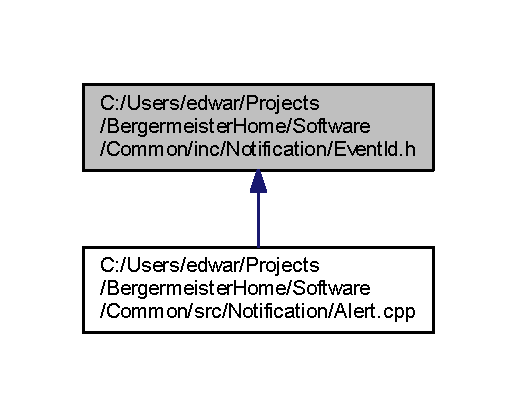
\includegraphics[width=248pt]{_event_id_8h__dep__incl}
\end{center}
\end{figure}
\subsection*{Namespaces}
\begin{DoxyCompactItemize}
\item 
 \mbox{\hyperlink{namespace_g_n_common}{G\+N\+Common}}
\begin{DoxyCompactList}\small\item\em Namespace containing Common components and infrastrucutre. \end{DoxyCompactList}\item 
 \mbox{\hyperlink{namespace_g_n_common_1_1_n_notification}{G\+N\+Common\+::\+N\+Notification}}
\begin{DoxyCompactList}\small\item\em Namespace containing system Alerts. \end{DoxyCompactList}\end{DoxyCompactItemize}
\subsection*{Enumerations}
\begin{DoxyCompactItemize}
\item 
enum \mbox{\hyperlink{namespace_g_n_common_1_1_n_notification_a8d5ce0e5fbb0a6cdcd96e4b037656761}{G\+N\+Common\+::\+N\+Notification\+::\+Tc\+Event\+Id}} \+: Tu32 \{ {\bfseries Xe\+Identifier}, 
{\bfseries Xe\+Status}, 
{\bfseries Xe\+Timestamp}, 
{\bfseries Xe\+Data}
 \}
\end{DoxyCompactItemize}


\subsection{Detailed Description}
Package interface for the Event Identifier Enumeration. 



Definition in file \mbox{\hyperlink{_event_id_8h_source}{Event\+Id.\+h}}.


\hypertarget{_event_id_8h_source}{}\section{Event\+Id.\+h}
\label{_event_id_8h_source}\index{C\+:/\+Users/edwar/\+Projects/\+Bergermeister\+Home/\+Software/\+Common/inc/\+Notification/\+Event\+Id.\+h@{C\+:/\+Users/edwar/\+Projects/\+Bergermeister\+Home/\+Software/\+Common/inc/\+Notification/\+Event\+Id.\+h}}

\begin{DoxyCode}
00001 
00005 \textcolor{preprocessor}{#pragma once}
00006 
00007 \textcolor{keyword}{namespace }\mbox{\hyperlink{namespace_g_n_common}{GNCommon}}
00008 \{
00009    \textcolor{keyword}{namespace }NNotification
00010    \{
\Hypertarget{_event_id_8h_source_l00012}\mbox{\hyperlink{namespace_g_n_common_1_1_n_notification_a8d5ce0e5fbb0a6cdcd96e4b037656761}{00012}}       \textcolor{keyword}{enum class} \mbox{\hyperlink{namespace_g_n_common_1_1_n_notification_a8d5ce0e5fbb0a6cdcd96e4b037656761}{TcEventId}} : \mbox{\hyperlink{namespace_g_n_common_a941b527ef318f318aed7903dc832b7e4}{Tu32}}
00013       \{
00014          XeIdentifier,
00015          XeStatus,
00016          XeTimestamp,
00017          XeData
00018       \};
00019    \}
00020 \}
00021 
\end{DoxyCode}

\hypertarget{_group_id_8h}{}\section{C\+:/\+Projects/\+Bergermeister\+Home/\+Software/\+Common/inc/\+Notification/\+Group\+Id.h File Reference}
\label{_group_id_8h}\index{C\+:/\+Projects/\+Bergermeister\+Home/\+Software/\+Common/inc/\+Notification/\+Group\+Id.\+h@{C\+:/\+Projects/\+Bergermeister\+Home/\+Software/\+Common/inc/\+Notification/\+Group\+Id.\+h}}


Package interface for the Group Identifier Enumeration.  


\subsection*{Namespaces}
\begin{DoxyCompactItemize}
\item 
 \mbox{\hyperlink{namespace_g_n_common}{G\+N\+Common}}
\begin{DoxyCompactList}\small\item\em Namespace containing Common components and infrastrucutre. \end{DoxyCompactList}\item 
 \mbox{\hyperlink{namespace_g_n_common_1_1_n_notification}{G\+N\+Common\+::\+N\+Notification}}
\begin{DoxyCompactList}\small\item\em Namespace containing system Alerts. \end{DoxyCompactList}\end{DoxyCompactItemize}
\subsection*{Enumerations}
\begin{DoxyCompactItemize}
\item 
enum \mbox{\hyperlink{namespace_g_n_common_1_1_n_notification_af29017ad6ed59156beabc385a91db18e}{G\+N\+Common\+::\+N\+Notification\+::\+Tc\+Group\+Id}} \+: Tu8 \{ \mbox{\hyperlink{namespace_g_n_common_1_1_n_notification_af29017ad6ed59156beabc385a91db18eab1dd4ba140ef44b2b6e425a90b4d11ba}{G\+N\+Common\+::\+N\+Notification\+::\+Tc\+Group\+Id\+::\+Xe\+None}} = 0, 
\mbox{\hyperlink{namespace_g_n_common_1_1_n_notification_af29017ad6ed59156beabc385a91db18eaf127afdc99e6a03185eab77f17740359}{G\+N\+Common\+::\+N\+Notification\+::\+Tc\+Group\+Id\+::\+Xe\+Network}} = 1
 \}
\end{DoxyCompactItemize}


\subsection{Detailed Description}
Package interface for the Group Identifier Enumeration. 



Definition in file \mbox{\hyperlink{_group_id_8h_source}{Group\+Id.\+h}}.


\hypertarget{_group_id_8h_source}{}\section{Group\+Id.\+h}
\label{_group_id_8h_source}\index{C\+:/\+Users/edwar/\+Projects/\+Bergermeister\+Home/\+Software/\+Common/inc/\+Notification/\+Group\+Id.\+h@{C\+:/\+Users/edwar/\+Projects/\+Bergermeister\+Home/\+Software/\+Common/inc/\+Notification/\+Group\+Id.\+h}}

\begin{DoxyCode}
00001 
00005 \textcolor{preprocessor}{#pragma once}
00006 
00007 \textcolor{keyword}{namespace }\mbox{\hyperlink{namespace_g_n_common}{GNCommon}}
00008 \{
00009    \textcolor{keyword}{namespace }NNotification
00010    \{
\Hypertarget{_group_id_8h_source_l00012}\mbox{\hyperlink{namespace_g_n_common_1_1_n_notification_af29017ad6ed59156beabc385a91db18e}{00012}}       \textcolor{keyword}{enum class} \mbox{\hyperlink{namespace_g_n_common_1_1_n_notification_af29017ad6ed59156beabc385a91db18e}{TcGroupId}} : \mbox{\hyperlink{namespace_g_n_common_a7939e251ddbf5d3a31832dcfdc8bde39}{Tu8}}
00013       \{
00014          \mbox{\hyperlink{namespace_g_n_common_1_1_n_notification_ab468f440599e6d5a51d887dfa55b06b3ab1dd4ba140ef44b2b6e425a90b4d11ba}{XeNone}}    = 0, 
00015          \mbox{\hyperlink{namespace_g_n_common_1_1_n_notification_af29017ad6ed59156beabc385a91db18eaf127afdc99e6a03185eab77f17740359}{XeNetwork}} = 1  
00016       \};
00017    \}
00018 \}
\end{DoxyCode}

\hypertarget{_identifier_8h}{}\section{C\+:/\+Projects/\+Bergermeister\+Home/\+Software/\+Common/inc/\+Notification/\+Identifier.h File Reference}
\label{_identifier_8h}\index{C\+:/\+Projects/\+Bergermeister\+Home/\+Software/\+Common/inc/\+Notification/\+Identifier.\+h@{C\+:/\+Projects/\+Bergermeister\+Home/\+Software/\+Common/inc/\+Notification/\+Identifier.\+h}}


Package interface for the Alert Identifier.  


{\ttfamily \#include $<$Types.\+h$>$}\newline
{\ttfamily \#include $<$Notification\textbackslash{}\+Group\+Id.\+h$>$}\newline
{\ttfamily \#include $<$Notification\textbackslash{}\+Component\+Id.\+h$>$}\newline
\subsection*{Classes}
\begin{DoxyCompactItemize}
\item 
class \mbox{\hyperlink{class_g_n_common_1_1_n_notification_1_1_tc_identifier}{G\+N\+Common\+::\+N\+Notification\+::\+Tc\+Identifier}}
\end{DoxyCompactItemize}
\subsection*{Namespaces}
\begin{DoxyCompactItemize}
\item 
 \mbox{\hyperlink{namespace_g_n_common}{G\+N\+Common}}
\begin{DoxyCompactList}\small\item\em Namespace containing Common components and infrastrucutre. \end{DoxyCompactList}\item 
 \mbox{\hyperlink{namespace_g_n_common_1_1_n_notification}{G\+N\+Common\+::\+N\+Notification}}
\begin{DoxyCompactList}\small\item\em Namespace containing system Alerts. \end{DoxyCompactList}\end{DoxyCompactItemize}


\subsection{Detailed Description}
Package interface for the Alert Identifier. 



Definition in file \mbox{\hyperlink{_identifier_8h_source}{Identifier.\+h}}.


\hypertarget{_identifier_8h_source}{}\section{Identifier.\+h}
\label{_identifier_8h_source}\index{C\+:/\+Projects/\+Bergermeister\+Home/\+Software/\+Common/inc/\+Notification/\+Identifier.\+h@{C\+:/\+Projects/\+Bergermeister\+Home/\+Software/\+Common/inc/\+Notification/\+Identifier.\+h}}

\begin{DoxyCode}
00001 
00005 \textcolor{preprocessor}{#pragma once}
00006 
00007 \textcolor{preprocessor}{#include <\mbox{\hyperlink{_types_8h}{Types.h}}>}
00008 \textcolor{preprocessor}{#include <\mbox{\hyperlink{_group_id_8h}{Notification\(\backslash\)GroupId.h}}>}
00009 \textcolor{preprocessor}{#include <\mbox{\hyperlink{_component_id_8h}{Notification\(\backslash\)ComponentId.h}}>}
00010 
00011 \textcolor{keyword}{namespace }\mbox{\hyperlink{namespace_g_n_common}{GNCommon}}
00012 \{
00013    \textcolor{keyword}{namespace }NNotification
00014    \{
\Hypertarget{_identifier_8h_source_l00016}\mbox{\hyperlink{class_g_n_common_1_1_n_notification_1_1_tc_identifier}{00016}}       \textcolor{keyword}{class }\mbox{\hyperlink{class_g_n_common_1_1_n_notification_1_1_tc_identifier}{TcIdentifier}}
00017       \{
00018       \textcolor{keyword}{public}:        \textcolor{comment}{// Public Attributes}
\Hypertarget{_identifier_8h_source_l00019}\mbox{\hyperlink{class_g_n_common_1_1_n_notification_1_1_tc_identifier_a704ac106036ca2d6b4fae77be75e7913}{00019}}          \mbox{\hyperlink{namespace_g_n_common_a7939e251ddbf5d3a31832dcfdc8bde39}{Tu8}}           \mbox{\hyperlink{class_g_n_common_1_1_n_notification_1_1_tc_identifier_a704ac106036ca2d6b4fae77be75e7913}{vucIndex}};  
\Hypertarget{_identifier_8h_source_l00020}\mbox{\hyperlink{class_g_n_common_1_1_n_notification_1_1_tc_identifier_afcf493852b92439dca37c671b549c2d3}{00020}}          \mbox{\hyperlink{namespace_g_n_common_1_1_n_notification_af29017ad6ed59156beabc385a91db18e}{TcGroupId}}     \mbox{\hyperlink{class_g_n_common_1_1_n_notification_1_1_tc_identifier_afcf493852b92439dca37c671b549c2d3}{voGroup}};   
\Hypertarget{_identifier_8h_source_l00021}\mbox{\hyperlink{class_g_n_common_1_1_n_notification_1_1_tc_identifier_a226babb1936c6e0841174fd1baac3476}{00021}}          \mbox{\hyperlink{namespace_g_n_common_1_1_n_notification_ab468f440599e6d5a51d887dfa55b06b3}{TcComponentId}} \mbox{\hyperlink{class_g_n_common_1_1_n_notification_1_1_tc_identifier_a226babb1936c6e0841174fd1baac3476}{voCompDet}}; 
\Hypertarget{_identifier_8h_source_l00022}\mbox{\hyperlink{class_g_n_common_1_1_n_notification_1_1_tc_identifier_a259c70f5d04a2cb6e8c674a07f903aff}{00022}}          \mbox{\hyperlink{namespace_g_n_common_1_1_n_notification_ab468f440599e6d5a51d887dfa55b06b3}{TcComponentId}} \mbox{\hyperlink{class_g_n_common_1_1_n_notification_1_1_tc_identifier_a259c70f5d04a2cb6e8c674a07f903aff}{voCompGen}}; 
00024       \textcolor{keyword}{public}:        \textcolor{comment}{// Public Methods}
00025          \mbox{\hyperlink{class_g_n_common_1_1_n_notification_1_1_tc_identifier_a267c27d2c658da02dd9de307056e5957}{TcIdentifier}} ( \textcolor{keywordtype}{void} );
00026          \mbox{\hyperlink{class_g_n_common_1_1_n_notification_1_1_tc_identifier_a267c27d2c658da02dd9de307056e5957}{TcIdentifier}} ( \textcolor{keyword}{const} \mbox{\hyperlink{class_g_n_common_1_1_n_notification_1_1_tc_identifier}{TcIdentifier}}& aorIdentifier );
00027          \mbox{\hyperlink{class_g_n_common_1_1_n_notification_1_1_tc_identifier_a24a949696317f638bc14f2fe76443373}{~TcIdentifier}}( \textcolor{keywordtype}{void} );
00028          \mbox{\hyperlink{class_g_n_common_1_1_n_notification_1_1_tc_identifier}{TcIdentifier}}& \mbox{\hyperlink{class_g_n_common_1_1_n_notification_1_1_tc_identifier_a6a836e2b8afe92c207de676e574009ea}{operator=}}( \textcolor{keyword}{const} \mbox{\hyperlink{class_g_n_common_1_1_n_notification_1_1_tc_identifier}{TcIdentifier}}& aorIdentifier );
00029 
00030          \mbox{\hyperlink{namespace_g_n_common_a8115dc7ed53b6e5b52e6bfde1632ea74}{Tb8}} \mbox{\hyperlink{class_g_n_common_1_1_n_notification_1_1_tc_identifier_a1250350af717cc758d44354232acbc04}{operator==}}( \textcolor{keyword}{const} \mbox{\hyperlink{class_g_n_common_1_1_n_notification_1_1_tc_identifier}{TcIdentifier}}& aorIdentifier );
00031          \mbox{\hyperlink{namespace_g_n_common_a8115dc7ed53b6e5b52e6bfde1632ea74}{Tb8}} \mbox{\hyperlink{class_g_n_common_1_1_n_notification_1_1_tc_identifier_aaeba92963467ea1b7fb123094083633f}{operator!=}}( \textcolor{keyword}{const} \mbox{\hyperlink{class_g_n_common_1_1_n_notification_1_1_tc_identifier}{TcIdentifier}}& aorIdentifier );
00032       \};
00033    \}
00034 \}
\end{DoxyCode}

\hypertarget{_status_8h}{}\section{C\+:/\+Projects/\+Bergermeister\+Home/\+Software/\+Common/inc/\+Notification/\+Status.h File Reference}
\label{_status_8h}\index{C\+:/\+Projects/\+Bergermeister\+Home/\+Software/\+Common/inc/\+Notification/\+Status.\+h@{C\+:/\+Projects/\+Bergermeister\+Home/\+Software/\+Common/inc/\+Notification/\+Status.\+h}}


Package interface for the Alert Status.  


{\ttfamily \#include $<$Types.\+h$>$}\newline
{\ttfamily \#include $<$Notification\textbackslash{}\+Criticality.\+h$>$}\newline
\subsection*{Classes}
\begin{DoxyCompactItemize}
\item 
class \mbox{\hyperlink{class_g_n_common_1_1_n_notification_1_1_tc_status}{G\+N\+Common\+::\+N\+Notification\+::\+Tc\+Status}}
\end{DoxyCompactItemize}
\subsection*{Namespaces}
\begin{DoxyCompactItemize}
\item 
 \mbox{\hyperlink{namespace_g_n_common}{G\+N\+Common}}
\begin{DoxyCompactList}\small\item\em Namespace containing Common components and infrastrucutre. \end{DoxyCompactList}\item 
 \mbox{\hyperlink{namespace_g_n_common_1_1_n_notification}{G\+N\+Common\+::\+N\+Notification}}
\begin{DoxyCompactList}\small\item\em Namespace containing system Alerts. \end{DoxyCompactList}\end{DoxyCompactItemize}


\subsection{Detailed Description}
Package interface for the Alert Status. 



Definition in file \mbox{\hyperlink{_status_8h_source}{Status.\+h}}.


\hypertarget{_status_8h_source}{}\section{Status.\+h}
\label{_status_8h_source}\index{C\+:/\+Users/edwar/\+Projects/\+Bergermeister\+Home/\+Software/\+Common/inc/\+Notification/\+Status.\+h@{C\+:/\+Users/edwar/\+Projects/\+Bergermeister\+Home/\+Software/\+Common/inc/\+Notification/\+Status.\+h}}

\begin{DoxyCode}
00001 
00005 \textcolor{preprocessor}{#pragma once}
00006 
00007 \textcolor{preprocessor}{#include <\mbox{\hyperlink{_types_8h}{Types.h}}>}
00008 \textcolor{preprocessor}{#include <\mbox{\hyperlink{_criticality_8h}{Notification\(\backslash\)Criticality.h}}>}
00009 
00010 \textcolor{keyword}{namespace }\mbox{\hyperlink{namespace_g_n_common}{GNCommon}}
00011 \{
00012    \textcolor{keyword}{namespace }NNotification
00013    \{
\Hypertarget{_status_8h_source_l00015}\mbox{\hyperlink{class_g_n_common_1_1_n_notification_1_1_tc_status}{00015}}       \textcolor{keyword}{class }\mbox{\hyperlink{class_g_n_common_1_1_n_notification_1_1_tc_status}{TcStatus}}
00016       \{
00017       \textcolor{keyword}{public}:        \textcolor{comment}{// Public Attributes}
\Hypertarget{_status_8h_source_l00018}\mbox{\hyperlink{class_g_n_common_1_1_n_notification_1_1_tc_status_a69149fc8c4c5facf147993b95d171c10}{00018}}          \mbox{\hyperlink{namespace_g_n_common_a7939e251ddbf5d3a31832dcfdc8bde39}{Tu8}}           \mbox{\hyperlink{class_g_n_common_1_1_n_notification_1_1_tc_status_a69149fc8c4c5facf147993b95d171c10}{vucActive}}       : 1; 
\Hypertarget{_status_8h_source_l00019}\mbox{\hyperlink{class_g_n_common_1_1_n_notification_1_1_tc_status_a487d66407748b7a91d9d663c3fab0f2c}{00019}}          \mbox{\hyperlink{namespace_g_n_common_a7939e251ddbf5d3a31832dcfdc8bde39}{Tu8}}           \mbox{\hyperlink{class_g_n_common_1_1_n_notification_1_1_tc_status_a487d66407748b7a91d9d663c3fab0f2c}{vucAcknowledged}} : 1; 
\Hypertarget{_status_8h_source_l00020}\mbox{\hyperlink{class_g_n_common_1_1_n_notification_1_1_tc_status_a36e84f5ebb3fda08f3ddaccde0a1c37b}{00020}}          \mbox{\hyperlink{namespace_g_n_common_a7939e251ddbf5d3a31832dcfdc8bde39}{Tu8}}           \mbox{\hyperlink{class_g_n_common_1_1_n_notification_1_1_tc_status_a36e84f5ebb3fda08f3ddaccde0a1c37b}{vucCleared}}      : 1; 
\Hypertarget{_status_8h_source_l00021}\mbox{\hyperlink{class_g_n_common_1_1_n_notification_1_1_tc_status_a4af337a51278a09d8500bab15d929af3}{00021}}          \mbox{\hyperlink{namespace_g_n_common_a7939e251ddbf5d3a31832dcfdc8bde39}{Tu8}}           \mbox{\hyperlink{class_g_n_common_1_1_n_notification_1_1_tc_status_a4af337a51278a09d8500bab15d929af3}{vucTrigger}}      : 1; 
\Hypertarget{_status_8h_source_l00022}\mbox{\hyperlink{class_g_n_common_1_1_n_notification_1_1_tc_status_ad8eff97b5c02e0409d3cbc65bf65c313}{00022}}          \mbox{\hyperlink{namespace_g_n_common_a7939e251ddbf5d3a31832dcfdc8bde39}{Tu8}}           \mbox{\hyperlink{class_g_n_common_1_1_n_notification_1_1_tc_status_ad8eff97b5c02e0409d3cbc65bf65c313}{vucSpare1}}       : 4; 
\Hypertarget{_status_8h_source_l00023}\mbox{\hyperlink{class_g_n_common_1_1_n_notification_1_1_tc_status_a2f8cb2528ae8cba51e3acc7f28eb2eeb}{00023}}          \mbox{\hyperlink{namespace_g_n_common_1_1_n_notification_a7d5c0650483fe26fa420ae5bf787566b}{TcCriticality}} \mbox{\hyperlink{class_g_n_common_1_1_n_notification_1_1_tc_status_a2f8cb2528ae8cba51e3acc7f28eb2eeb}{voCriticality}};       
\Hypertarget{_status_8h_source_l00024}\mbox{\hyperlink{class_g_n_common_1_1_n_notification_1_1_tc_status_aaee139b3984634b3cc3cc7e2b7175035}{00024}}          \mbox{\hyperlink{namespace_g_n_common_a7939e251ddbf5d3a31832dcfdc8bde39}{Tu8}}           \mbox{\hyperlink{class_g_n_common_1_1_n_notification_1_1_tc_status_aaee139b3984634b3cc3cc7e2b7175035}{vucSpare2}};           
\Hypertarget{_status_8h_source_l00025}\mbox{\hyperlink{class_g_n_common_1_1_n_notification_1_1_tc_status_ae398de0e32d0352b0437f4267247fd6d}{00025}}          \mbox{\hyperlink{namespace_g_n_common_a7939e251ddbf5d3a31832dcfdc8bde39}{Tu8}}           \mbox{\hyperlink{class_g_n_common_1_1_n_notification_1_1_tc_status_ae398de0e32d0352b0437f4267247fd6d}{vucChildren}};         
00027       \textcolor{keyword}{public}:        \textcolor{comment}{// Public Methods}
00028          \mbox{\hyperlink{class_g_n_common_1_1_n_notification_1_1_tc_status_a43b5990228e5a9fbe9bfe63605f7a9d2}{TcStatus}} ( \textcolor{keywordtype}{void} );
00029          \mbox{\hyperlink{class_g_n_common_1_1_n_notification_1_1_tc_status_a43b5990228e5a9fbe9bfe63605f7a9d2}{TcStatus}} ( \textcolor{keyword}{const} \mbox{\hyperlink{class_g_n_common_1_1_n_notification_1_1_tc_status}{TcStatus}}& aorStatus );
00030          \mbox{\hyperlink{class_g_n_common_1_1_n_notification_1_1_tc_status_af14caf8abaf597904cebb6d414fd1dcf}{~TcStatus}}( \textcolor{keywordtype}{void} );
00031          \mbox{\hyperlink{class_g_n_common_1_1_n_notification_1_1_tc_status}{TcStatus}}& \mbox{\hyperlink{class_g_n_common_1_1_n_notification_1_1_tc_status_a97c8135ccc33bc5ba9d33f79de4ea789}{operator=}}( \textcolor{keyword}{const} \mbox{\hyperlink{class_g_n_common_1_1_n_notification_1_1_tc_status}{TcStatus}}& aorStatus );
00032 
00033          \mbox{\hyperlink{namespace_g_n_common_a8115dc7ed53b6e5b52e6bfde1632ea74}{Tb8}} \mbox{\hyperlink{class_g_n_common_1_1_n_notification_1_1_tc_status_acf4e836982c2da53ad1e6989af623c58}{operator==}}( \textcolor{keyword}{const} \mbox{\hyperlink{class_g_n_common_1_1_n_notification_1_1_tc_status}{TcStatus}}& aorStatus );
00034          \mbox{\hyperlink{namespace_g_n_common_a8115dc7ed53b6e5b52e6bfde1632ea74}{Tb8}} \mbox{\hyperlink{class_g_n_common_1_1_n_notification_1_1_tc_status_acdf1eba6040e3cd5e244e21524ff0d86}{operator!=}}( \textcolor{keyword}{const} \mbox{\hyperlink{class_g_n_common_1_1_n_notification_1_1_tc_status}{TcStatus}}& aorStatus );
00035       \};
00036    \}
00037 \}
\end{DoxyCode}

\hypertarget{_stop_watch_8h}{}\section{C\+:/\+Projects/\+Bergermeister\+Home/\+Software/\+Common/inc/\+Stop\+Watch.h File Reference}
\label{_stop_watch_8h}\index{C\+:/\+Projects/\+Bergermeister\+Home/\+Software/\+Common/inc/\+Stop\+Watch.\+h@{C\+:/\+Projects/\+Bergermeister\+Home/\+Software/\+Common/inc/\+Stop\+Watch.\+h}}
\subsection*{Classes}
\begin{DoxyCompactItemize}
\item 
class \mbox{\hyperlink{class_g_n_common_1_1_g_tc_stop_watch}{G\+N\+Common\+::\+G\+Tc\+Stop\+Watch}}
\end{DoxyCompactItemize}
\subsection*{Namespaces}
\begin{DoxyCompactItemize}
\item 
 \mbox{\hyperlink{namespace_g_n_common}{G\+N\+Common}}
\begin{DoxyCompactList}\small\item\em Namespace containing Common components and infrastrucutre. \end{DoxyCompactList}\end{DoxyCompactItemize}


\subsection{Detailed Description}
Package interface for the Stop Watch class interface 

Definition in file \mbox{\hyperlink{_stop_watch_8h_source}{Stop\+Watch.\+h}}.


\hypertarget{_stop_watch_8h_source}{}\section{Stop\+Watch.\+h}
\label{_stop_watch_8h_source}\index{C\+:/\+Projects/\+Bergermeister\+Home/\+Software/\+Common/inc/\+Stop\+Watch.\+h@{C\+:/\+Projects/\+Bergermeister\+Home/\+Software/\+Common/inc/\+Stop\+Watch.\+h}}

\begin{DoxyCode}
00001 
00006 \textcolor{preprocessor}{#pragma once}
00007 
00008 \textcolor{keyword}{namespace }\mbox{\hyperlink{namespace_g_n_common}{GNCommon}}
00009 \{
\Hypertarget{_stop_watch_8h_source_l00010}\mbox{\hyperlink{class_g_n_common_1_1_g_tc_stop_watch}{00010}}    \textcolor{keyword}{class }\mbox{\hyperlink{class_g_n_common_1_1_g_tc_stop_watch}{GTcStopWatch}}
00011    \{
00012    \textcolor{keyword}{protected}:     \textcolor{comment}{// Protected Attributes}
00013       \textcolor{keyword}{static} \textcolor{keyword}{const} \mbox{\hyperlink{namespace_g_n_common_ad0a34f67eefe81cfbd0e515bba246d9d}{Ti64}} xlMaxQuadPart = 9223372036854775807;  
\Hypertarget{_stop_watch_8h_source_l00014}\mbox{\hyperlink{class_g_n_common_1_1_g_tc_stop_watch_a525b6eebced7d4d9c3812788cfde2b75}{00014}}       \textcolor{keyword}{static} \textcolor{keyword}{const} \mbox{\hyperlink{namespace_g_n_common_a9404ee6090c788ae70aebd1436ceb97d}{Tu64}} \mbox{\hyperlink{class_g_n_common_1_1_g_tc_stop_watch_a525b6eebced7d4d9c3812788cfde2b75}{xulTimeBase}}   = 1000000LL;            
00015       \textcolor{keyword}{static} \mbox{\hyperlink{namespace_g_n_common_a9404ee6090c788ae70aebd1436ceb97d}{Tu64}} vulFrequency;
00016 
00017       \mbox{\hyperlink{namespace_g_n_common_ad0a34f67eefe81cfbd0e515bba246d9d}{Ti64}} vlStart;
00018       \mbox{\hyperlink{namespace_g_n_common_ad0a34f67eefe81cfbd0e515bba246d9d}{Ti64}} vlEnd;
00019       \mbox{\hyperlink{namespace_g_n_common_a8115dc7ed53b6e5b52e6bfde1632ea74}{Tb8}}  vbRunning;
00020 
00021    \textcolor{keyword}{public}:
00022       \mbox{\hyperlink{class_g_n_common_1_1_g_tc_stop_watch}{GTcStopWatch}}( \textcolor{keywordtype}{void} );
00023       \mbox{\hyperlink{class_g_n_common_1_1_g_tc_stop_watch}{GTcStopWatch}}( \textcolor{keyword}{const} \mbox{\hyperlink{class_g_n_common_1_1_g_tc_stop_watch}{GTcStopWatch}}& aorStopWatch );
00024       ~\mbox{\hyperlink{class_g_n_common_1_1_g_tc_stop_watch}{GTcStopWatch}}( \textcolor{keywordtype}{void} );
00025 
00026       \mbox{\hyperlink{class_g_n_common_1_1_g_tc_stop_watch}{GTcStopWatch}}& operator=( \textcolor{keyword}{const} \mbox{\hyperlink{class_g_n_common_1_1_g_tc_stop_watch}{GTcStopWatch}}& aorStopWatch );
00027 
00028       \textcolor{keywordtype}{void}  MStart  ( \textcolor{keywordtype}{void} );
00029       \mbox{\hyperlink{namespace_g_n_common_a9404ee6090c788ae70aebd1436ceb97d}{Tu64}} MStop   ( \textcolor{keywordtype}{void} );
00030       \mbox{\hyperlink{namespace_g_n_common_a9404ee6090c788ae70aebd1436ceb97d}{Tu64}} MElapsed( \textcolor{keywordtype}{void} );
00031    \};
00032 
00033 \}
00034 
\end{DoxyCode}

\hypertarget{_types_8h}{}\section{C\+:/\+Users/edwar/\+Projects/\+Bergermeister\+Home/\+Software/\+Common/inc/\+Types.h File Reference}
\label{_types_8h}\index{C\+:/\+Users/edwar/\+Projects/\+Bergermeister\+Home/\+Software/\+Common/inc/\+Types.\+h@{C\+:/\+Users/edwar/\+Projects/\+Bergermeister\+Home/\+Software/\+Common/inc/\+Types.\+h}}


Commnon Framework namespace, type definitions, and coding style guide Defines the common namespace (\mbox{\hyperlink{namespace_g_n_common}{G\+N\+Common}}), common primitive types, and provides the style guide to be used.  


This graph shows which files directly or indirectly include this file\+:
\nopagebreak
\begin{figure}[H]
\begin{center}
\leavevmode
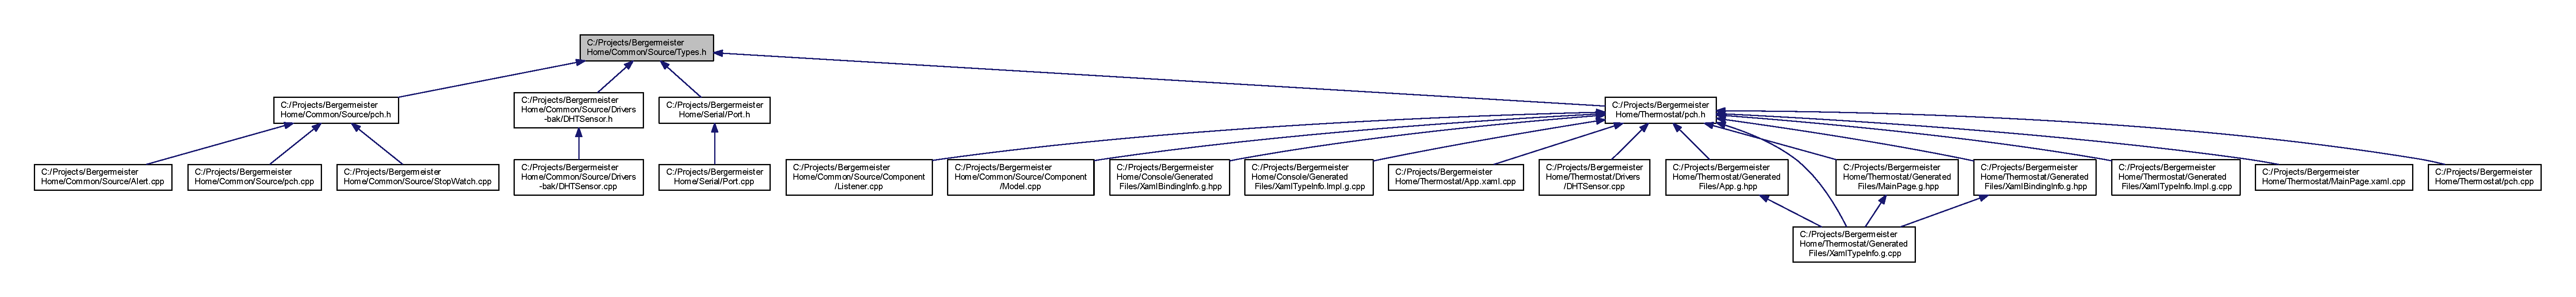
\includegraphics[width=350pt]{_types_8h__dep__incl}
\end{center}
\end{figure}
\subsection*{Namespaces}
\begin{DoxyCompactItemize}
\item 
 \mbox{\hyperlink{namespace_g_n_common}{G\+N\+Common}}
\begin{DoxyCompactList}\small\item\em Namespace containing Common components and infrastrucutre. \end{DoxyCompactList}\end{DoxyCompactItemize}
\subsection*{Typedefs}
\begin{DoxyCompactItemize}
\item 
typedef bool \mbox{\hyperlink{namespace_g_n_common_a8115dc7ed53b6e5b52e6bfde1632ea74}{G\+N\+Common\+::\+Tb8}}
\item 
typedef char \mbox{\hyperlink{namespace_g_n_common_a2d8d4c56e54519697c6ee80cc1ceda76}{G\+N\+Common\+::\+Tc8}}
\item 
typedef signed char \mbox{\hyperlink{namespace_g_n_common_a9bac2aa36db6d72a3e59b1869adf3668}{G\+N\+Common\+::\+Ti8}}
\item 
typedef unsigned char \mbox{\hyperlink{namespace_g_n_common_a7939e251ddbf5d3a31832dcfdc8bde39}{G\+N\+Common\+::\+Tu8}}
\item 
typedef signed short \mbox{\hyperlink{namespace_g_n_common_ab9a9a6aa84751cec965d8b6676318a65}{G\+N\+Common\+::\+Ti16}}
\item 
typedef unsigned short \mbox{\hyperlink{namespace_g_n_common_a7f651a58155939d1e0e2bf2164fbfdbf}{G\+N\+Common\+::\+Tu16}}
\item 
typedef signed long \mbox{\hyperlink{namespace_g_n_common_ad1f094ce51908947ac3d31355b560d55}{G\+N\+Common\+::\+Ti32}}
\item 
typedef unsigned long \mbox{\hyperlink{namespace_g_n_common_a941b527ef318f318aed7903dc832b7e4}{G\+N\+Common\+::\+Tu32}}
\item 
typedef signed long long \mbox{\hyperlink{namespace_g_n_common_ad0a34f67eefe81cfbd0e515bba246d9d}{G\+N\+Common\+::\+Ti64}}
\item 
typedef unsigned long long \mbox{\hyperlink{namespace_g_n_common_a9404ee6090c788ae70aebd1436ceb97d}{G\+N\+Common\+::\+Tu64}}
\item 
typedef float \mbox{\hyperlink{namespace_g_n_common_ae4ffdde6236eb7578669b280a5d1634d}{G\+N\+Common\+::\+Tf32}}
\item 
typedef double \mbox{\hyperlink{namespace_g_n_common_a73af96f1663fd8fc5741bcbc5b1427e4}{G\+N\+Common\+::\+Tf64}}
\end{DoxyCompactItemize}


\subsection{Detailed Description}
Commnon Framework namespace, type definitions, and coding style guide Defines the common namespace (\mbox{\hyperlink{namespace_g_n_common}{G\+N\+Common}}), common primitive types, and provides the style guide to be used. 

\begin{DoxyVerb}* Style Guide
*
*  (S)cope:                                
*                | Priv  |  Pub  | Global |
*                |-------|-------|--------|
* Class Variable |   v   |   V   |  ----  |
* Stack Variable |   k   |  ---  |  ----  | 
*       Argument |   a   |  ---  |  ----  |
*        Typedef |   t   |   T   |   GT   |
*   Constant ROM |   x   |   X   |   GX   |
*         Method |   m   |   M   |   GM   |
*                                          
*  (T)ype:                                 
*           | Prefix |                     
*           |--------|                     
*      Tb8 |    b   |                     
*      Tc8 |    c   |                     
*      Ti8 |    c   |                     
*      Tu8 |   uc   |                     
*     Ti16 |    s   |                     
*     Tu16 |   us   |                     
*     Ti32 |    i   |                     
*     Tu32 |   ui   |                     
*     Ti64 |    l   |                     
*     Tu64 |   ul   |                     
*     Tf32 |    f   |                     
*     Tf64 |    d   |                     
*                                          
*  (O)perator:                             
*               | Prefix |                 
*               |--------|                 
*     pointer   |    p   |                 
*     reference |    r   |                 
*                                          
*  Naming Convention:                      
*     STOCamelCaseName                     
*     GMFunctionGlobal
* \end{DoxyVerb}
 

Definition in file \mbox{\hyperlink{_types_8h_source}{Types.\+h}}.


\hypertarget{_types_8h_source}{}\section{Types.\+h}
\label{_types_8h_source}\index{C\+:/\+Users/edwar/\+Projects/\+Bergermeister\+Home/\+Software/\+Common/inc/\+Types.\+h@{C\+:/\+Users/edwar/\+Projects/\+Bergermeister\+Home/\+Software/\+Common/inc/\+Types.\+h}}

\begin{DoxyCode}
00001 
00048 \textcolor{preprocessor}{#pragma once}
00049 
00051 \textcolor{keyword}{namespace }\mbox{\hyperlink{namespace_g_n_common}{GNCommon}}
00052 \{
00053    
\Hypertarget{_types_8h_source_l00054}\mbox{\hyperlink{namespace_g_n_common_a8115dc7ed53b6e5b52e6bfde1632ea74}{00054}}    \textcolor{keyword}{typedef}               \textcolor{keywordtype}{bool}  \mbox{\hyperlink{namespace_g_n_common_a8115dc7ed53b6e5b52e6bfde1632ea74}{Tb8}}; 
\Hypertarget{_types_8h_source_l00055}\mbox{\hyperlink{namespace_g_n_common_a2d8d4c56e54519697c6ee80cc1ceda76}{00055}}    \textcolor{keyword}{typedef}               \textcolor{keywordtype}{char}  \mbox{\hyperlink{namespace_g_n_common_a2d8d4c56e54519697c6ee80cc1ceda76}{Tc8}}; 
\Hypertarget{_types_8h_source_l00056}\mbox{\hyperlink{namespace_g_n_common_a9bac2aa36db6d72a3e59b1869adf3668}{00056}}    \textcolor{keyword}{typedef} \textcolor{keywordtype}{signed}        \textcolor{keywordtype}{char}  \mbox{\hyperlink{namespace_g_n_common_a9bac2aa36db6d72a3e59b1869adf3668}{Ti8}}; 
\Hypertarget{_types_8h_source_l00057}\mbox{\hyperlink{namespace_g_n_common_a7939e251ddbf5d3a31832dcfdc8bde39}{00057}}    \textcolor{keyword}{typedef} \textcolor{keywordtype}{unsigned}      \textcolor{keywordtype}{char}  \mbox{\hyperlink{namespace_g_n_common_a7939e251ddbf5d3a31832dcfdc8bde39}{Tu8}}; 
\Hypertarget{_types_8h_source_l00058}\mbox{\hyperlink{namespace_g_n_common_ab9a9a6aa84751cec965d8b6676318a65}{00058}}    \textcolor{keyword}{typedef} \textcolor{keywordtype}{signed}       \textcolor{keywordtype}{short} \mbox{\hyperlink{namespace_g_n_common_ab9a9a6aa84751cec965d8b6676318a65}{Ti16}}; 
\Hypertarget{_types_8h_source_l00059}\mbox{\hyperlink{namespace_g_n_common_a7f651a58155939d1e0e2bf2164fbfdbf}{00059}}    \textcolor{keyword}{typedef} \textcolor{keywordtype}{unsigned}     \textcolor{keywordtype}{short} \mbox{\hyperlink{namespace_g_n_common_a7f651a58155939d1e0e2bf2164fbfdbf}{Tu16}}; 
\Hypertarget{_types_8h_source_l00060}\mbox{\hyperlink{namespace_g_n_common_ad1f094ce51908947ac3d31355b560d55}{00060}}    \textcolor{keyword}{typedef} \textcolor{keywordtype}{signed}        \textcolor{keywordtype}{long} \mbox{\hyperlink{namespace_g_n_common_ad1f094ce51908947ac3d31355b560d55}{Ti32}}; 
\Hypertarget{_types_8h_source_l00061}\mbox{\hyperlink{namespace_g_n_common_a941b527ef318f318aed7903dc832b7e4}{00061}}    \textcolor{keyword}{typedef} \textcolor{keywordtype}{unsigned}      \textcolor{keywordtype}{long} \mbox{\hyperlink{namespace_g_n_common_a941b527ef318f318aed7903dc832b7e4}{Tu32}}; 
\Hypertarget{_types_8h_source_l00062}\mbox{\hyperlink{namespace_g_n_common_ad0a34f67eefe81cfbd0e515bba246d9d}{00062}}    \textcolor{keyword}{typedef} \textcolor{keywordtype}{signed}   \textcolor{keywordtype}{long} \textcolor{keywordtype}{long} \mbox{\hyperlink{namespace_g_n_common_ad0a34f67eefe81cfbd0e515bba246d9d}{Ti64}}; 
\Hypertarget{_types_8h_source_l00063}\mbox{\hyperlink{namespace_g_n_common_a9404ee6090c788ae70aebd1436ceb97d}{00063}}    \textcolor{keyword}{typedef} \textcolor{keywordtype}{unsigned} \textcolor{keywordtype}{long} \textcolor{keywordtype}{long} \mbox{\hyperlink{namespace_g_n_common_a9404ee6090c788ae70aebd1436ceb97d}{Tu64}}; 
\Hypertarget{_types_8h_source_l00064}\mbox{\hyperlink{namespace_g_n_common_ae4ffdde6236eb7578669b280a5d1634d}{00064}}    \textcolor{keyword}{typedef}              \textcolor{keywordtype}{float} \mbox{\hyperlink{namespace_g_n_common_ae4ffdde6236eb7578669b280a5d1634d}{Tf32}}; 
\Hypertarget{_types_8h_source_l00065}\mbox{\hyperlink{namespace_g_n_common_a73af96f1663fd8fc5741bcbc5b1427e4}{00065}}    \textcolor{keyword}{typedef}             \textcolor{keywordtype}{double} \mbox{\hyperlink{namespace_g_n_common_a73af96f1663fd8fc5741bcbc5b1427e4}{Tf64}}; 
00067    \textcolor{keyword}{static} \textcolor{keyword}{const} \mbox{\hyperlink{namespace_g_n_common_a941b527ef318f318aed7903dc832b7e4}{Tu32}} XuiSizeOfTb8  = \textcolor{keyword}{sizeof}( \mbox{\hyperlink{namespace_g_n_common_a8115dc7ed53b6e5b52e6bfde1632ea74}{Tb8}} );  
00068    \textcolor{keyword}{static} \textcolor{keyword}{const} \mbox{\hyperlink{namespace_g_n_common_a941b527ef318f318aed7903dc832b7e4}{Tu32}} XuiSizeOfTi8  = \textcolor{keyword}{sizeof}( \mbox{\hyperlink{namespace_g_n_common_a9bac2aa36db6d72a3e59b1869adf3668}{Ti8}} );  
00069    \textcolor{keyword}{static} \textcolor{keyword}{const} \mbox{\hyperlink{namespace_g_n_common_a941b527ef318f318aed7903dc832b7e4}{Tu32}} XuiSizeOfTu8  = \textcolor{keyword}{sizeof}( \mbox{\hyperlink{namespace_g_n_common_a7939e251ddbf5d3a31832dcfdc8bde39}{Tu8}} );  
00070    \textcolor{keyword}{static} \textcolor{keyword}{const} \mbox{\hyperlink{namespace_g_n_common_a941b527ef318f318aed7903dc832b7e4}{Tu32}} XuiSizeOfTi16 = \textcolor{keyword}{sizeof}( \mbox{\hyperlink{namespace_g_n_common_ab9a9a6aa84751cec965d8b6676318a65}{Ti16}} ); 
00071    \textcolor{keyword}{static} \textcolor{keyword}{const} \mbox{\hyperlink{namespace_g_n_common_a941b527ef318f318aed7903dc832b7e4}{Tu32}} XuiSizeOfTu16 = \textcolor{keyword}{sizeof}( \mbox{\hyperlink{namespace_g_n_common_a7f651a58155939d1e0e2bf2164fbfdbf}{Tu16}} ); 
00072    \textcolor{keyword}{static} \textcolor{keyword}{const} \mbox{\hyperlink{namespace_g_n_common_a941b527ef318f318aed7903dc832b7e4}{Tu32}} XuiSizeOfTi32 = \textcolor{keyword}{sizeof}( \mbox{\hyperlink{namespace_g_n_common_ad1f094ce51908947ac3d31355b560d55}{Ti32}} ); 
00073    \textcolor{keyword}{static} \textcolor{keyword}{const} \mbox{\hyperlink{namespace_g_n_common_a941b527ef318f318aed7903dc832b7e4}{Tu32}} XuiSizeOfTu32 = \textcolor{keyword}{sizeof}( \mbox{\hyperlink{namespace_g_n_common_a941b527ef318f318aed7903dc832b7e4}{Tu32}} ); 
00074    \textcolor{keyword}{static} \textcolor{keyword}{const} \mbox{\hyperlink{namespace_g_n_common_a941b527ef318f318aed7903dc832b7e4}{Tu32}} XuiSizeOfTi64 = \textcolor{keyword}{sizeof}( \mbox{\hyperlink{namespace_g_n_common_ad0a34f67eefe81cfbd0e515bba246d9d}{Ti64}} ); 
00075    \textcolor{keyword}{static} \textcolor{keyword}{const} \mbox{\hyperlink{namespace_g_n_common_a941b527ef318f318aed7903dc832b7e4}{Tu32}} XuiSizeOfTu64 = \textcolor{keyword}{sizeof}( \mbox{\hyperlink{namespace_g_n_common_a9404ee6090c788ae70aebd1436ceb97d}{Tu64}} ); 
00076    \textcolor{keyword}{static} \textcolor{keyword}{const} \mbox{\hyperlink{namespace_g_n_common_a941b527ef318f318aed7903dc832b7e4}{Tu32}} XuiSizeOfTf32 = \textcolor{keyword}{sizeof}( \mbox{\hyperlink{namespace_g_n_common_a9404ee6090c788ae70aebd1436ceb97d}{Tu64}} ); 
00077    \textcolor{keyword}{static} \textcolor{keyword}{const} \mbox{\hyperlink{namespace_g_n_common_a941b527ef318f318aed7903dc832b7e4}{Tu32}} XuiSizeOfTf64 = \textcolor{keyword}{sizeof}( \mbox{\hyperlink{namespace_g_n_common_a9404ee6090c788ae70aebd1436ceb97d}{Tu64}} ); 
00078 \}
\end{DoxyCode}

\hypertarget{_identifier_8cpp}{}\section{C\+:/\+Users/edwar/\+Projects/\+Bergermeister\+Home/\+Software/\+Common/src/\+Notification/\+Identifier.cpp File Reference}
\label{_identifier_8cpp}\index{C\+:/\+Users/edwar/\+Projects/\+Bergermeister\+Home/\+Software/\+Common/src/\+Notification/\+Identifier.\+cpp@{C\+:/\+Users/edwar/\+Projects/\+Bergermeister\+Home/\+Software/\+Common/src/\+Notification/\+Identifier.\+cpp}}
{\ttfamily \#include $<$Types.\+h$>$}\newline
{\ttfamily \#include $<$Notification\textbackslash{}\+Group\+Id.\+h$>$}\newline
{\ttfamily \#include $<$Notification\textbackslash{}\+Component\+Id.\+h$>$}\newline
{\ttfamily \#include $<$Notification\textbackslash{}\+Identifier.\+h$>$}\newline
Include dependency graph for Identifier.\+cpp\+:
\nopagebreak
\begin{figure}[H]
\begin{center}
\leavevmode
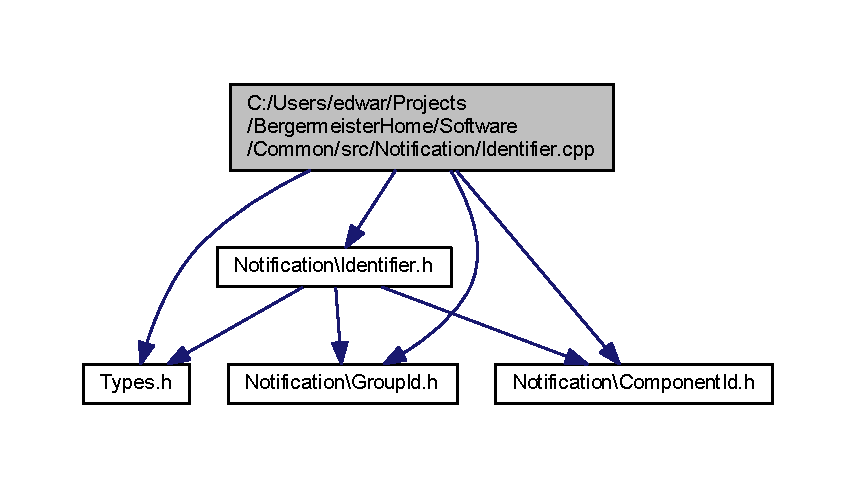
\includegraphics[width=350pt]{_identifier_8cpp__incl}
\end{center}
\end{figure}


\subsection{Detailed Description}
Package implementation for the Alert Identifier 

Definition in file \mbox{\hyperlink{_identifier_8cpp_source}{Identifier.\+cpp}}.


\hypertarget{_identifier_8cpp_source}{}\section{Identifier.\+cpp}
\label{_identifier_8cpp_source}\index{C\+:/\+Users/edwar/\+Projects/\+Bergermeister\+Home/\+Software/\+Common/src/\+Notification/\+Identifier.\+cpp@{C\+:/\+Users/edwar/\+Projects/\+Bergermeister\+Home/\+Software/\+Common/src/\+Notification/\+Identifier.\+cpp}}

\begin{DoxyCode}
00001 
00006 \textcolor{preprocessor}{#include <\mbox{\hyperlink{_types_8h}{Types.h}}>}
00007 \textcolor{preprocessor}{#include <\mbox{\hyperlink{_group_id_8h}{Notification\(\backslash\)GroupId.h}}>}
00008 \textcolor{preprocessor}{#include <\mbox{\hyperlink{_component_id_8h}{Notification\(\backslash\)ComponentId.h}}>}
00009 \textcolor{preprocessor}{#include <\mbox{\hyperlink{_identifier_8h}{Notification\(\backslash\)Identifier.h}}>}
00010 
00011 \textcolor{keyword}{using namespace }\mbox{\hyperlink{namespace_g_n_common}{GNCommon}};
00012 \textcolor{keyword}{using namespace }\mbox{\hyperlink{namespace_g_n_common_1_1_n_notification}{GNCommon::NNotification}};
00013 
\Hypertarget{_identifier_8cpp_source_l00027}\mbox{\hyperlink{class_g_n_common_1_1_n_notification_1_1_tc_identifier_a267c27d2c658da02dd9de307056e5957}{00027}} \mbox{\hyperlink{class_g_n_common_1_1_n_notification_1_1_tc_identifier_a267c27d2c658da02dd9de307056e5957}{TcIdentifier::TcIdentifier}}( \textcolor{keywordtype}{void} )
00028 \{
00029    this->\mbox{\hyperlink{class_g_n_common_1_1_n_notification_1_1_tc_identifier_a704ac106036ca2d6b4fae77be75e7913}{vucIndex}}  = 0;
00030    this->\mbox{\hyperlink{class_g_n_common_1_1_n_notification_1_1_tc_identifier_afcf493852b92439dca37c671b549c2d3}{voGroup}}   = \mbox{\hyperlink{namespace_g_n_common_1_1_n_notification_ab468f440599e6d5a51d887dfa55b06b3ab1dd4ba140ef44b2b6e425a90b4d11ba}{TcGroupId::XeNone}};    
00031    this->\mbox{\hyperlink{class_g_n_common_1_1_n_notification_1_1_tc_identifier_a226babb1936c6e0841174fd1baac3476}{voCompDet}} = \mbox{\hyperlink{namespace_g_n_common_1_1_n_notification_ab468f440599e6d5a51d887dfa55b06b3ab1dd4ba140ef44b2b6e425a90b4d11ba}{TcComponentId::XeNone}};
00032    this->\mbox{\hyperlink{class_g_n_common_1_1_n_notification_1_1_tc_identifier_a259c70f5d04a2cb6e8c674a07f903aff}{voCompGen}} = \mbox{\hyperlink{namespace_g_n_common_1_1_n_notification_ab468f440599e6d5a51d887dfa55b06b3ab1dd4ba140ef44b2b6e425a90b4d11ba}{TcComponentId::XeNone}};
00033 \}
00034 
\Hypertarget{_identifier_8cpp_source_l00048}\mbox{\hyperlink{class_g_n_common_1_1_n_notification_1_1_tc_identifier_a38728e27be5fd22296b49b76bdda619b}{00048}} \mbox{\hyperlink{class_g_n_common_1_1_n_notification_1_1_tc_identifier_a267c27d2c658da02dd9de307056e5957}{TcIdentifier::TcIdentifier}}( \textcolor{keyword}{const} \mbox{\hyperlink{class_g_n_common_1_1_n_notification_1_1_tc_identifier}{TcIdentifier}}& aorIdentifier )
00049 \{
00050    *\textcolor{keyword}{this} = aorIdentifier;
00051 \}
00052 
\Hypertarget{_identifier_8cpp_source_l00066}\mbox{\hyperlink{class_g_n_common_1_1_n_notification_1_1_tc_identifier_a24a949696317f638bc14f2fe76443373}{00066}} \mbox{\hyperlink{class_g_n_common_1_1_n_notification_1_1_tc_identifier_a24a949696317f638bc14f2fe76443373}{TcIdentifier::~TcIdentifier}}( \textcolor{keywordtype}{void} )
00067 \{
00068    \textcolor{comment}{// Nothing to Destruct}
00069 \}
00070 
\Hypertarget{_identifier_8cpp_source_l00084}\mbox{\hyperlink{class_g_n_common_1_1_n_notification_1_1_tc_identifier_a6a836e2b8afe92c207de676e574009ea}{00084}} \mbox{\hyperlink{class_g_n_common_1_1_n_notification_1_1_tc_identifier}{TcIdentifier}}& \mbox{\hyperlink{class_g_n_common_1_1_n_notification_1_1_tc_identifier_a6a836e2b8afe92c207de676e574009ea}{TcIdentifier::operator=}}( \textcolor{keyword}{const} 
      \mbox{\hyperlink{class_g_n_common_1_1_n_notification_1_1_tc_identifier}{TcIdentifier}}& aorIdentifier )
00085 \{
00086    this->\mbox{\hyperlink{class_g_n_common_1_1_n_notification_1_1_tc_identifier_a704ac106036ca2d6b4fae77be75e7913}{vucIndex}}  = aorIdentifier.\mbox{\hyperlink{class_g_n_common_1_1_n_notification_1_1_tc_identifier_a704ac106036ca2d6b4fae77be75e7913}{vucIndex}};
00087    this->\mbox{\hyperlink{class_g_n_common_1_1_n_notification_1_1_tc_identifier_afcf493852b92439dca37c671b549c2d3}{voGroup}}   = aorIdentifier.\mbox{\hyperlink{class_g_n_common_1_1_n_notification_1_1_tc_identifier_afcf493852b92439dca37c671b549c2d3}{voGroup}};
00088    this->\mbox{\hyperlink{class_g_n_common_1_1_n_notification_1_1_tc_identifier_a226babb1936c6e0841174fd1baac3476}{voCompDet}} = aorIdentifier.\mbox{\hyperlink{class_g_n_common_1_1_n_notification_1_1_tc_identifier_a226babb1936c6e0841174fd1baac3476}{voCompDet}};
00089    this->\mbox{\hyperlink{class_g_n_common_1_1_n_notification_1_1_tc_identifier_a259c70f5d04a2cb6e8c674a07f903aff}{voCompGen}} = aorIdentifier.\mbox{\hyperlink{class_g_n_common_1_1_n_notification_1_1_tc_identifier_a259c70f5d04a2cb6e8c674a07f903aff}{voCompGen}};
00090 
00091    \textcolor{keywordflow}{return}( *\textcolor{keyword}{this} );
00092 \}
00093 
\Hypertarget{_identifier_8cpp_source_l00107}\mbox{\hyperlink{class_g_n_common_1_1_n_notification_1_1_tc_identifier_a1250350af717cc758d44354232acbc04}{00107}} \mbox{\hyperlink{namespace_g_n_common_a8115dc7ed53b6e5b52e6bfde1632ea74}{Tb8}} \mbox{\hyperlink{class_g_n_common_1_1_n_notification_1_1_tc_identifier_a1250350af717cc758d44354232acbc04}{TcIdentifier::operator==}}( \textcolor{keyword}{const} \mbox{\hyperlink{class_g_n_common_1_1_n_notification_1_1_tc_identifier}{TcIdentifier}}& aorIdentifier )
00108 \{
00109    \mbox{\hyperlink{namespace_g_n_common_a8115dc7ed53b6e5b52e6bfde1632ea74}{Tb8}} kbEqual = \textcolor{keyword}{true}; \textcolor{comment}{// Assume Equal}
00110 
00111    \textcolor{keywordflow}{if} ( ( this->\mbox{\hyperlink{class_g_n_common_1_1_n_notification_1_1_tc_identifier_a704ac106036ca2d6b4fae77be75e7913}{vucIndex}}  != aorIdentifier.\mbox{\hyperlink{class_g_n_common_1_1_n_notification_1_1_tc_identifier_a704ac106036ca2d6b4fae77be75e7913}{vucIndex}}  ) ||
00112         ( this->voGroup   != aorIdentifier.\mbox{\hyperlink{class_g_n_common_1_1_n_notification_1_1_tc_identifier_afcf493852b92439dca37c671b549c2d3}{voGroup}}   ) ||
00113         ( this->voCompDet != aorIdentifier.\mbox{\hyperlink{class_g_n_common_1_1_n_notification_1_1_tc_identifier_a226babb1936c6e0841174fd1baac3476}{voCompDet}} ) ||
00114         ( this->voCompGen != aorIdentifier.\mbox{\hyperlink{class_g_n_common_1_1_n_notification_1_1_tc_identifier_a259c70f5d04a2cb6e8c674a07f903aff}{voCompGen}} ) )
00115    \{
00116       kbEqual = \textcolor{keyword}{false};
00117    \}
00118 
00119    \textcolor{keywordflow}{return}( kbEqual );
00120 \}
00121 
\Hypertarget{_identifier_8cpp_source_l00135}\mbox{\hyperlink{class_g_n_common_1_1_n_notification_1_1_tc_identifier_aaeba92963467ea1b7fb123094083633f}{00135}} \mbox{\hyperlink{namespace_g_n_common_a8115dc7ed53b6e5b52e6bfde1632ea74}{Tb8}} \mbox{\hyperlink{class_g_n_common_1_1_n_notification_1_1_tc_identifier_aaeba92963467ea1b7fb123094083633f}{TcIdentifier::operator!=}}( \textcolor{keyword}{const} \mbox{\hyperlink{class_g_n_common_1_1_n_notification_1_1_tc_identifier}{TcIdentifier}}& aorIdentifier )
00136 \{
00137    \textcolor{keywordflow}{return}( !( *\textcolor{keyword}{this} == aorIdentifier ) );
00138 \}
00139 
\end{DoxyCode}

\hypertarget{_status_8cpp}{}\section{C\+:/\+Projects/\+Bergermeister\+Home/\+Software/\+Common/src/\+Notification/\+Status.cpp File Reference}
\label{_status_8cpp}\index{C\+:/\+Projects/\+Bergermeister\+Home/\+Software/\+Common/src/\+Notification/\+Status.\+cpp@{C\+:/\+Projects/\+Bergermeister\+Home/\+Software/\+Common/src/\+Notification/\+Status.\+cpp}}


Package implementation for the Alert Status.  


{\ttfamily \#include $<$Types.\+h$>$}\newline
{\ttfamily \#include $<$Notification\textbackslash{}\+Criticality.\+h$>$}\newline
{\ttfamily \#include $<$Notification\textbackslash{}\+Status.\+h$>$}\newline


\subsection{Detailed Description}
Package implementation for the Alert Status. 



Definition in file \mbox{\hyperlink{_status_8cpp_source}{Status.\+cpp}}.


\hypertarget{_status_8cpp_source}{}\section{Status.\+cpp}
\label{_status_8cpp_source}\index{C\+:/\+Users/edwar/\+Projects/\+Bergermeister\+Home/\+Software/\+Common/src/\+Notification/\+Status.\+cpp@{C\+:/\+Users/edwar/\+Projects/\+Bergermeister\+Home/\+Software/\+Common/src/\+Notification/\+Status.\+cpp}}

\begin{DoxyCode}
00001 
00005 \textcolor{preprocessor}{#include <\mbox{\hyperlink{_types_8h}{Types.h}}>}
00006 \textcolor{preprocessor}{#include <\mbox{\hyperlink{_criticality_8h}{Notification\(\backslash\)Criticality.h}}>}
00007 \textcolor{preprocessor}{#include <\mbox{\hyperlink{_status_8h}{Notification\(\backslash\)Status.h}}>}
00008 
00009 \textcolor{keyword}{using namespace }\mbox{\hyperlink{namespace_g_n_common}{GNCommon}};
00010 \textcolor{keyword}{using namespace }\mbox{\hyperlink{namespace_g_n_common_1_1_n_notification}{GNCommon::NNotification}};
00011 
\Hypertarget{_status_8cpp_source_l00025}\mbox{\hyperlink{class_g_n_common_1_1_n_notification_1_1_tc_status_a43b5990228e5a9fbe9bfe63605f7a9d2}{00025}} \mbox{\hyperlink{class_g_n_common_1_1_n_notification_1_1_tc_status_a43b5990228e5a9fbe9bfe63605f7a9d2}{TcStatus::TcStatus}}( \textcolor{keywordtype}{void} )
00026 \{
00027    this->\mbox{\hyperlink{class_g_n_common_1_1_n_notification_1_1_tc_status_a69149fc8c4c5facf147993b95d171c10}{vucActive}}       = \textcolor{keyword}{false};
00028    this->\mbox{\hyperlink{class_g_n_common_1_1_n_notification_1_1_tc_status_a487d66407748b7a91d9d663c3fab0f2c}{vucAcknowledged}} = \textcolor{keyword}{false};
00029    this->\mbox{\hyperlink{class_g_n_common_1_1_n_notification_1_1_tc_status_a36e84f5ebb3fda08f3ddaccde0a1c37b}{vucCleared}}      = \textcolor{keyword}{false};
00030    this->\mbox{\hyperlink{class_g_n_common_1_1_n_notification_1_1_tc_status_a4af337a51278a09d8500bab15d929af3}{vucTrigger}}      = \textcolor{keyword}{false};
00031    this->\mbox{\hyperlink{class_g_n_common_1_1_n_notification_1_1_tc_status_ad8eff97b5c02e0409d3cbc65bf65c313}{vucSpare1}}       = 0;
00032    this->\mbox{\hyperlink{class_g_n_common_1_1_n_notification_1_1_tc_status_a2f8cb2528ae8cba51e3acc7f28eb2eeb}{voCriticality}}   = \mbox{\hyperlink{namespace_g_n_common_1_1_n_notification_ab468f440599e6d5a51d887dfa55b06b3ab1dd4ba140ef44b2b6e425a90b4d11ba}{TcCriticality::XeNone}};
00033    this->\mbox{\hyperlink{class_g_n_common_1_1_n_notification_1_1_tc_status_aaee139b3984634b3cc3cc7e2b7175035}{vucSpare2}}       = 0;
00034    this->\mbox{\hyperlink{class_g_n_common_1_1_n_notification_1_1_tc_status_ae398de0e32d0352b0437f4267247fd6d}{vucChildren}}     = 0;
00035 \}
00036 
\Hypertarget{_status_8cpp_source_l00050}\mbox{\hyperlink{class_g_n_common_1_1_n_notification_1_1_tc_status_abfb0ff092f9a23017fc89dcd1d6f4e6f}{00050}} \mbox{\hyperlink{class_g_n_common_1_1_n_notification_1_1_tc_status_a43b5990228e5a9fbe9bfe63605f7a9d2}{TcStatus::TcStatus}}( \textcolor{keyword}{const} \mbox{\hyperlink{class_g_n_common_1_1_n_notification_1_1_tc_status}{TcStatus}}& aorStatus )
00051 \{
00052    *\textcolor{keyword}{this} = aorStatus;
00053 \}
00054 
\Hypertarget{_status_8cpp_source_l00068}\mbox{\hyperlink{class_g_n_common_1_1_n_notification_1_1_tc_status_af14caf8abaf597904cebb6d414fd1dcf}{00068}} \mbox{\hyperlink{class_g_n_common_1_1_n_notification_1_1_tc_status_af14caf8abaf597904cebb6d414fd1dcf}{TcStatus::~TcStatus}}( \textcolor{keywordtype}{void} )
00069 \{
00070    \textcolor{comment}{// Nothing to destruct}
00071 \}
00072 
00073 
\Hypertarget{_status_8cpp_source_l00087}\mbox{\hyperlink{class_g_n_common_1_1_n_notification_1_1_tc_status_a97c8135ccc33bc5ba9d33f79de4ea789}{00087}} \mbox{\hyperlink{class_g_n_common_1_1_n_notification_1_1_tc_status}{TcStatus}}& \mbox{\hyperlink{class_g_n_common_1_1_n_notification_1_1_tc_status_a97c8135ccc33bc5ba9d33f79de4ea789}{TcStatus::operator=}}( \textcolor{keyword}{const} \mbox{\hyperlink{class_g_n_common_1_1_n_notification_1_1_tc_status}{TcStatus}}& aorStatus )
00088 \{
00089    this->\mbox{\hyperlink{class_g_n_common_1_1_n_notification_1_1_tc_status_a69149fc8c4c5facf147993b95d171c10}{vucActive}}       = aorStatus.\mbox{\hyperlink{class_g_n_common_1_1_n_notification_1_1_tc_status_a69149fc8c4c5facf147993b95d171c10}{vucActive}};
00090    this->\mbox{\hyperlink{class_g_n_common_1_1_n_notification_1_1_tc_status_a487d66407748b7a91d9d663c3fab0f2c}{vucAcknowledged}} = aorStatus.\mbox{\hyperlink{class_g_n_common_1_1_n_notification_1_1_tc_status_a487d66407748b7a91d9d663c3fab0f2c}{vucAcknowledged}};
00091    this->\mbox{\hyperlink{class_g_n_common_1_1_n_notification_1_1_tc_status_a36e84f5ebb3fda08f3ddaccde0a1c37b}{vucCleared}}      = aorStatus.\mbox{\hyperlink{class_g_n_common_1_1_n_notification_1_1_tc_status_a36e84f5ebb3fda08f3ddaccde0a1c37b}{vucCleared}};
00092    this->\mbox{\hyperlink{class_g_n_common_1_1_n_notification_1_1_tc_status_a4af337a51278a09d8500bab15d929af3}{vucTrigger}}      = aorStatus.\mbox{\hyperlink{class_g_n_common_1_1_n_notification_1_1_tc_status_a4af337a51278a09d8500bab15d929af3}{vucTrigger}};
00093    this->\mbox{\hyperlink{class_g_n_common_1_1_n_notification_1_1_tc_status_ad8eff97b5c02e0409d3cbc65bf65c313}{vucSpare1}}       = aorStatus.\mbox{\hyperlink{class_g_n_common_1_1_n_notification_1_1_tc_status_ad8eff97b5c02e0409d3cbc65bf65c313}{vucSpare1}};
00094    this->\mbox{\hyperlink{class_g_n_common_1_1_n_notification_1_1_tc_status_a2f8cb2528ae8cba51e3acc7f28eb2eeb}{voCriticality}}   = aorStatus.\mbox{\hyperlink{class_g_n_common_1_1_n_notification_1_1_tc_status_a2f8cb2528ae8cba51e3acc7f28eb2eeb}{voCriticality}};
00095    this->\mbox{\hyperlink{class_g_n_common_1_1_n_notification_1_1_tc_status_aaee139b3984634b3cc3cc7e2b7175035}{vucSpare2}}       = aorStatus.\mbox{\hyperlink{class_g_n_common_1_1_n_notification_1_1_tc_status_aaee139b3984634b3cc3cc7e2b7175035}{vucSpare2}};
00096    this->\mbox{\hyperlink{class_g_n_common_1_1_n_notification_1_1_tc_status_ae398de0e32d0352b0437f4267247fd6d}{vucChildren}}     = aorStatus.\mbox{\hyperlink{class_g_n_common_1_1_n_notification_1_1_tc_status_ae398de0e32d0352b0437f4267247fd6d}{vucChildren}};
00097 
00098    \textcolor{keywordflow}{return}( *\textcolor{keyword}{this} );
00099 \}
00100 
\Hypertarget{_status_8cpp_source_l00114}\mbox{\hyperlink{class_g_n_common_1_1_n_notification_1_1_tc_status_acf4e836982c2da53ad1e6989af623c58}{00114}} \mbox{\hyperlink{namespace_g_n_common_a8115dc7ed53b6e5b52e6bfde1632ea74}{Tb8}} \mbox{\hyperlink{class_g_n_common_1_1_n_notification_1_1_tc_status_acf4e836982c2da53ad1e6989af623c58}{TcStatus::operator==}}( \textcolor{keyword}{const} \mbox{\hyperlink{class_g_n_common_1_1_n_notification_1_1_tc_status}{TcStatus}}& aorStatus )
00115 \{
00116    \mbox{\hyperlink{namespace_g_n_common_a8115dc7ed53b6e5b52e6bfde1632ea74}{Tb8}} kbEqual = \textcolor{keyword}{true}; \textcolor{comment}{// Assume Equal}
00117 
00118    \textcolor{keywordflow}{if} ( ( this->\mbox{\hyperlink{class_g_n_common_1_1_n_notification_1_1_tc_status_a69149fc8c4c5facf147993b95d171c10}{vucActive}}       != aorStatus.\mbox{\hyperlink{class_g_n_common_1_1_n_notification_1_1_tc_status_a69149fc8c4c5facf147993b95d171c10}{vucActive}}       ) ||
00119         ( this->vucAcknowledged != aorStatus.\mbox{\hyperlink{class_g_n_common_1_1_n_notification_1_1_tc_status_a487d66407748b7a91d9d663c3fab0f2c}{vucAcknowledged}} ) ||
00120         ( this->vucCleared      != aorStatus.\mbox{\hyperlink{class_g_n_common_1_1_n_notification_1_1_tc_status_a36e84f5ebb3fda08f3ddaccde0a1c37b}{vucCleared}}      ) ||
00121         ( this->vucTrigger      != aorStatus.\mbox{\hyperlink{class_g_n_common_1_1_n_notification_1_1_tc_status_a4af337a51278a09d8500bab15d929af3}{vucTrigger}}      ) ||
00122         ( this->vucSpare1       != aorStatus.\mbox{\hyperlink{class_g_n_common_1_1_n_notification_1_1_tc_status_ad8eff97b5c02e0409d3cbc65bf65c313}{vucSpare1}}       ) ||
00123         ( this->voCriticality   != aorStatus.\mbox{\hyperlink{class_g_n_common_1_1_n_notification_1_1_tc_status_a2f8cb2528ae8cba51e3acc7f28eb2eeb}{voCriticality}}   ) ||
00124         ( this->vucSpare2       != aorStatus.\mbox{\hyperlink{class_g_n_common_1_1_n_notification_1_1_tc_status_aaee139b3984634b3cc3cc7e2b7175035}{vucSpare2}}       ) ||
00125         ( this->vucChildren     != aorStatus.\mbox{\hyperlink{class_g_n_common_1_1_n_notification_1_1_tc_status_ae398de0e32d0352b0437f4267247fd6d}{vucChildren}}     ) )
00126    \{
00127       kbEqual = \textcolor{keyword}{false};
00128    \}
00129 
00130    \textcolor{keywordflow}{return}( kbEqual );
00131 \}
00132 
\Hypertarget{_status_8cpp_source_l00146}\mbox{\hyperlink{class_g_n_common_1_1_n_notification_1_1_tc_status_acdf1eba6040e3cd5e244e21524ff0d86}{00146}} \mbox{\hyperlink{namespace_g_n_common_a8115dc7ed53b6e5b52e6bfde1632ea74}{Tb8}} \mbox{\hyperlink{class_g_n_common_1_1_n_notification_1_1_tc_status_acdf1eba6040e3cd5e244e21524ff0d86}{TcStatus::operator!=}}( \textcolor{keyword}{const} \mbox{\hyperlink{class_g_n_common_1_1_n_notification_1_1_tc_status}{TcStatus}}& aorStatus )
00147 \{
00148    \textcolor{keywordflow}{return}( !( *\textcolor{keyword}{this} == aorStatus ) );
00149 \}
00150 
\end{DoxyCode}

%--- End generated contents ---

% Index
\backmatter
\newpage
\phantomsection
\clearemptydoublepage
\addcontentsline{toc}{chapter}{Index}
\printindex

\end{document}
